

\graphicspath{{figures/geometry/}}
\chapter{Vectors and Geometry in Two and Three Dimensions}\label{chap geometry}
\chaptermark{Vectors and Geometry}

Before we get started doing calculus in two and three dimensions 
we need to brush up on some basic geometry, that we will use a lot. 
We are already familiar with the Cartesian plane\footnote{Ren\'e Descartes
(1596--1650) was a French scientist and philosopher, who lived in the Dutch Republic for roughly twenty years after serving in the (mercenary) Dutch States Army.
He is viewed as the father of analytic geometry, which uses numbers
to study geometry.},  but we'll start from the beginning.

\section{Points}\label{sec points}

Each point in two dimensions may be labeled by two coordinates\footnote{This is why the $xy$-plane is called ``two dimensional'' --- the name of each point consists of two real numbers.}
$(x,y)$ which specify the position of the point in some units with respect
to some axes as in the figure below. 
\begin{efig}
\begin{center}
   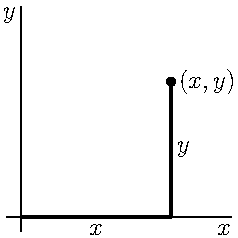
\includegraphics{point2d.pdf}
\end{center}
\end{efig}
The set of all points in two dimensions is denoted\footnote{Not surprisingly,
the $2$ in $\bbbr^2$ signifies that each point is labelled by two numbers
and the $\bbbr$ in $\bbbr^2$ signifies that the numbers in question are
real numbers. There are more advanced applications (for example in
signal analysis and in quantum mechanics) where complex numbers are used.
The space of all pairs $(z_1,z_2)$, with $z_1$ and $z_2$ complex numbers 
is denoted  $\bbbc^2$.} $\bbbr^2$.
Observe that 
\begin{itemize}\itemsep1pt \parskip0pt \parsep0pt
\item the distance from the point $(x,y)$ to the $x$-axis is $|y|$
\item if $y>0$, then $(x,y)$ is above the $x$-axis and if $y<0$, then
        $(x,y)$ is below the $x$-axis
\item the distance from the point $(x,y)$ to the $y$-axis is $|x|$
\item if $x>0$, then $(x,y)$ is the right of the $y$-axis and if $x<0$, then
        $(x,y)$ is to the left of the $y$-axis
\item the distance from the point $(x,y)$ to the origin $(0,0)$ is 
     $\sqrt{x^2+y^2}$
\end{itemize}

Similarly, each point in three dimensions may be labeled by 
three coordinates $(x,y,z)$, as in the two figures below.
\begin{efig}
\begin{center}
   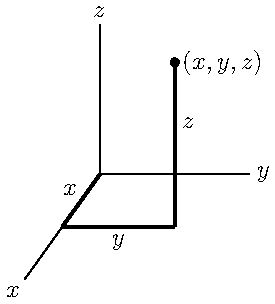
\includegraphics{point3d.pdf}\qquad
   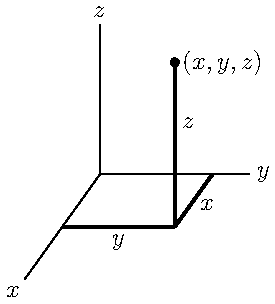
\includegraphics{point3db.pdf}
\end{center}
\end{efig}
The set of all points in three dimensions is denoted $\bbbr^3$.
The plane that contains, for example, the $x$- and $y$-axes
is called the $xy$-plane.
\begin{itemize}\itemsep1pt \parskip0pt \parsep0pt
\item The $xy$-plane is the set of all points $(x,y,z)$ that
satisfy $z=0$.
\item The $xz$-plane is the set of all points $(x,y,z)$ that
satisfy $y=0$.
\item The $yz$-plane is the set of all points $(x,y,z)$ that
satisfy $x=0$.
\end{itemize}
More generally,
\begin{itemize}\itemsep1pt \parskip0pt \parsep0pt
\item The set of all points $(x,y,z)$ that obey $z=c$ is a plane
that is parallel to the $xy$-plane and is a distance $|c|$ from it. 
If $c>0$, the plane $z=c$ is above the $xy$-plane.
If $c<0$, the plane $z=c$ is below the $xy$-plane.
We say that the plane $z=c$ is a signed distance $c$ from the
$xy$-plane.

\item The set of all points $(x,y,z)$ that obey $y=b$ is a plane
that is parallel to the $xz$-plane and is a signed distance $b$ from it. 

\item The set of all points $(x,y,z)$ that obey $x=a$ is a plane
that is parallel to the $yz$-plane and is a signed distance $a$ from it. 
\end{itemize}
\begin{efig}
\begin{center}
   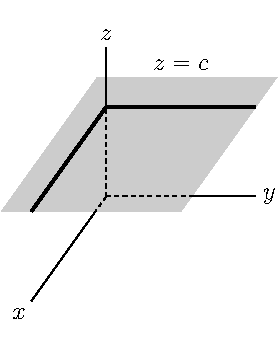
\includegraphics[scale=0.75]{xyplaneN.pdf}\qquad
   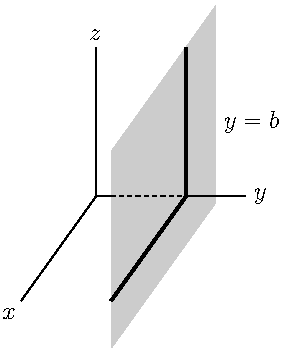
\includegraphics[scale=0.75]{xzplaneN.pdf}\qquad
   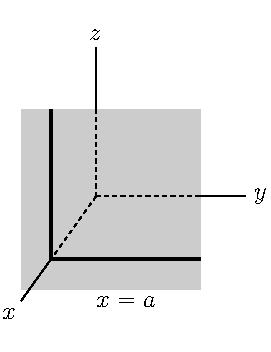
\includegraphics[scale=0.75]{yzplaneN.pdf}
\end{center}
\end{efig}
Observe that our 2d distances extend quite easily to 3d.
\begin{itemize}\itemsep1pt \parskip0pt \parsep0pt
\item the distance from the point $(x,y,z)$ to the $xy$-plane is $|z|$
\item the distance from the point $(x,y,z)$ to the $xz$-plane is $|y|$
\item the distance from the point $(x,y,z)$ to the $yz$-plane is $|x|$
\item the distance from the point $(x,y,z)$ to the origin $(0,0,0)$ is 
     $\sqrt{x^2+y^2+z^2}$
\end{itemize}
To see that the distance from the point $(x,y,z)$ to the origin $(0,0,0)$ 
is indeed  $\sqrt{x^2+y^2+z^2}$,
\begin{itemize}\itemsep1pt \parskip0pt \parsep0pt
\item 
apply Pythagoras to the right-angled triangle with vertices $(0,0,0)$,
$(x,0,0)$ and $(x,y,0)$ to see that the distance from $(0,0,0)$
to $(x,y,0)$ is $\sqrt{x^2+y^2}$ and then
\item 
apply Pythagoras to the right-angled triangle with vertices $(0,0,0)$,
$(x,y,0)$ and $(x,y,z)$ to see that the distance from $(0,0,0)$
to $(x,y,z)$ is $\sqrt{{\big(\sqrt{x^2+y^2}\big)}^2+z^2}
=\sqrt{x^2+y^2+z^2}$.
\end{itemize}
\begin{efig}
\begin{center}
   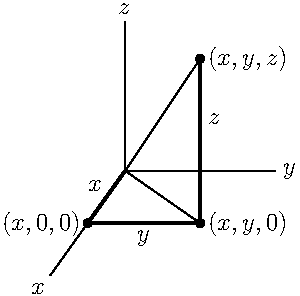
\includegraphics{pythag3d.pdf}
\end{center}
\end{efig}
More generally, the distance from the point $(x,y,z)$ to the point 
$(x',y',z')$ is
\begin{equation*}
\sqrt{(x-x')^2+(y-y')^2+(z-z')^2}
\end{equation*}
Notice that this gives us the equation for a sphere quite directly. 
All the points on a sphere are equidistant from the centre of the sphere.
So, for example, the equation of the sphere centered on $(1,2,3)$ with 
radius $4$, that is, the set of all points $(x,y,z)$ whose distance 
from $(1,2,3)$ is $4$, is 
\begin{equation*}
(x-1)^2+(y-2)^2+(z-3)^2=16
\end{equation*}

Here is an example in which we sketch a region in the $xy$-plane that is specified using inequalities.

\begin{eg}
In this example, we sketch the region
\begin{equation*}
\Set{(x,y)}{ -12\le x^2-6x +y^2-4y \le -9,\ \ y\ge 1}
\end{equation*}
in the $xy$-plane.

We do so in two steps. In the first step, we sketch the curves
$x^2-6x +y^2-4y=-12$, $x^2-6x +y^2-4y=-9$, and $y=1$.
\begin{itemize}
\item
By completing squares, we see that the equation  $x^2-6x +y^2-4y=-12$ 
is equivalent to $(x-3)^2 +(y-2)^2 =1$, which is the circle of radius 
$1$ centred on $(3,2)$. It is sketched in the figure below.

\item
By completing squares, we see that the equation  $x^2-6x +y^2-4y=-9$ 
is equivalent to $(x-3)^2 +(y-2)^2 =4$, which is the circle of radius 
$2$ centred on $(3,2)$. It is sketched in the figure below.

\item
The point $(x,y)$ obeys $y=1$ if and only if it is a distance $1$ vertically above the $x$-axis. So $y=1$ is the line that is parallel to the $x$-axis and is one unit above it. This line is also  sketched in the figure below.
\end{itemize}

\begin{efig}
\begin{center}
   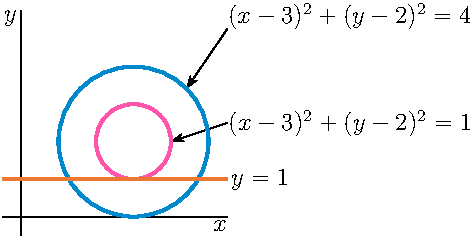
\includegraphics{annulusPart.pdf}
\end{center}
\end{efig}

In the second step we determine the impact that the inequalities have.
\begin{itemize}
\item 
The inequality $x^2-6x +y^2-4y\ge -12$ is equivalent to 
$(x-3)^2 +(y-2)^2 \ge 1$ and hence is equivalent to 
$\sqrt{(x-3)^2 +(y-2)^2} \ge 1$. So the point $(x,y)$ satisfies  
$x^2-6x +y^2-4y\ge -12$ if and only if the distance from $(x,y)$ to $(3,2)$
is at least $1$, i.e. if and only if $(x,y)$ is outside (or on) the circle 
$(x-3)^2 +(y-2)^2 = 1$. 

\item 
The inequality $x^2-6x +y^2-4y\le -9$ is equivalent to 
$(x-3)^2 +(y-2)^2 \le 4$ and hence is equivalent to 
$\sqrt{(x-3)^2 +(y-2)^2} \le 2$. So the point $(x,y)$ satisfies the inequality 
$x^2-6x +y^2-4y\le -9$ if and only if the distance from $(x,y)$ to $(3,2)$
is at most $2$, i.e. if and only if $(x,y)$ is inside (or on) the circle 
$(x-3)^2 +(y-2)^2 = 4$. 

\item 
The point $(x,y)$ obeys $y\ge 1$ if and only if $(x,y)$ is a vertical distance at least $1$ above the $x$-axis, i.e. is above (or on) the line $y=1$.

\item
So the region  
\begin{equation*}
\Set{(x,y)}{ -12\le x^2-6x +y^2-4y \le -9,\ \ y\ge 1}
\end{equation*}
consists of all points $(x,y)$ that 
\begin{itemize}
\item 
are inside or on the circle $(x-3)^2 +(y-2)^2 = 4$ and 
\item 
are also outside or on the circle $(x-3)^2 +(y-2)^2 = 1$ and 
\item 
are also above or on the line $y=1$. 
\end{itemize}
It is the shaded region in the figure below.
\end{itemize}

\begin{efig}
\begin{center}
   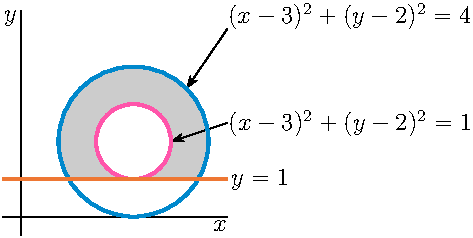
\includegraphics{annulusPartB.pdf}
\end{center}
\end{efig}

\end{eg}

Here are a couple of examples that involve spheres.

\begin{eg}
In this example, we are going to find the curve formed by the intersection of the $xy$-plane and the sphere of radius $5$ centred on $(0,0,4)$. 

The point $(x,y,z)$ lies on the $xy$-plane if and only if $z=0$, and lies on the  
sphere of radius $5$ centred on $(0,0,4)$ if and only if
$x^2+y^2+(z-4)^2=25$. So the point $(x,y,z)$ lies on the curve of intersection if and only if both $z=0$ and $x^2+y^2+(z-4)^2=25$, or equivalently
\begin{equation*}
z=0,\quad x^2+y^2+(0-4)^2=25
\iff
z=0,\quad x^2+y^2 = 9
\end{equation*}
This is the circle in the $xy$-plane that is centred on the origin and
has radius $3$. Here is a sketch that show the parts of the sphere 
and the circle of intersection that are in the first octant. That is, that
have $x\ge 0$, $y\ge 0$ and $z\ge 0$.
\begin{efig}
\begin{center}
   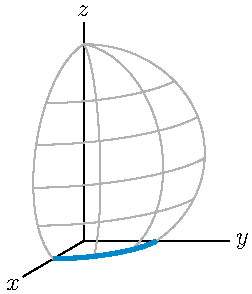
\includegraphics{sphereCircle.pdf}
\end{center}
\end{efig}
\end{eg}

\begin{eg}
In this example, we are going to find all points $(x,y,z)$ for which
the distance from $(x,y,z)$ to $(9,-12,15)$ is twice the distance from $(x,y,z)$   to the origin $(0,0,0)$.

The distance from $(x,y,z)$ to $(9,-12,15)$ is 
$\sqrt{(x-9)^2+(y+12)^2+(z-15)^2}$.
The distance from $(x,y,z)$ to $(0,0,0)$ is 
$\sqrt{x^2+y^2+z^2}$. So we want to find all points $(x,y,z)$ for which
\begin{equation*}
\sqrt{(x-9)^2+(y+12)^2+(z-15)^2}
=2\sqrt{x^2+y^2+z^2}
\end{equation*}
Squaring both sides of this equation gives
\begin{align*}
x^2-18x+81 +y^2+24y+144 +z^2-30z+225 &= 4\big(x^2+y^2+z^2)
\end{align*}
Collecting up terms gives
\begin{align*}
3x^2+18x +3y^2-24y +3z^2+30z &= 450\qquad\text{and then, dividing by $3$,} \\
x^2+6x +y^2-8y +z^2+10z &= 150\qquad\text{and then, completing squares,} \\
x^2+6x +9 +y^2-8y +16  +z^2+10z +25 &= 200\qquad\text{or}\\
(x+3)^2+(y-4)^2+(z+5)^2 &=200 
\end{align*}
This is the sphere of radius $10\sqrt{2}$ centred on $(-3,4,-5)$.
\end{eg}

%%%%%%%%%%%%%%%%%%%%%%%%
\section{Vectors}\label{sec vectors}
%%%%%%%%%%%%%%%%%%%%%%%%%
In many of our applications in 2d and 3d, we will encounter quantities
that have both a magnitude (like a distance) and also a 
direction. Such quantities are called vectors. That is,
a \emph{vector} is a quantity which has both a direction and a magnitude,
like a velocity. If you are moving, the magnitude (length) of your 
velocity vector is your speed (distance travelled per unit time)  and the
direction of your velocity vector is your direction of motion. To specify 
a vector in three dimensions you have to give three components, just as for 
a point. To draw the vector with components $\ a,\ b,\ c\ $ you can draw 
an arrow from the point $(0,0,0)$ to the point $(a,b,c)$. 
\vadjust{
      \begin{efig} 
      \begin{center}
      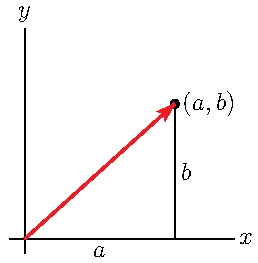
\includegraphics{vector2d.pdf} \qquad\qquad
      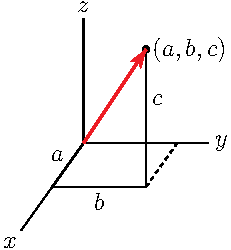
\includegraphics{vector3d.pdf}
      \end{center}
      \end{efig}
        }%
Similarly, to specify a vector in two dimensions
you have to give two components and to draw the vector
with components $\ a,\ b\ $ you can draw an arrow from the point $(0,0)$
to the point $(a,b)$.

There are many situations in which it is preferable to draw a vector 
with its tail at some point other than the origin. For example, it is 
natural to draw the velocity vector of a moving particle with the tail
of the velocity vector at the position of the particle, whether or not
the particle is at the origin. The sketch below shows a moving particle
and its velocity vector at two different times.
      \begin{efig} 
      \begin{center}
      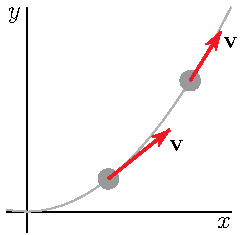
\includegraphics{movingParticle.pdf}
      \end{center}
      \end{efig}
As a second example, suppose that you are analyzing the motion of a pendulum.
There are three forces acting on the pendulum bob: gravity $\vg$, which
is pulling the bob straight down, tension $\vt$ in the rod, which is
pulling the bob in the direction of the rod, and air resistance $\vr$, 
which is pulling the bob in a direction opposite to its direction of motion.
All three forces are acting on the bob. So it is natural to draw all three
arrows representing the forces with their tails at the bob. 
      \begin{efig} 
      \begin{center}
      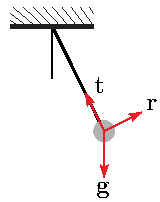
\includegraphics{pendulum.pdf}
      \end{center}
      \end{efig}

In this text, we will used bold faced letters, like $\vv$, $\vt$, $\vg$,
to designate vectors. In handwriting, it is clearer to use a small 
overhead arrow\footnote{Some people use an underline, as in $\underline{v}$,
rather than an arrow.}, as in $\vec{v}$, $\vec{t}$, $\vec{g}$, instead. 
Also, when we want to emphasise that some quantity is a number,
rather than a vector, we will call the number a \emph{scalar}. 


Both points and vectors in 2d are specified by two numbers. Until 
you get used to this, it might confuse you sometimes --- does a given pair of 
numbers represent a point or a vector?
To distinguish\footnote{Or, in the Wikipedia jargon, disambiguate.}
between the components of a vector and the coordinates 
of the point at its head, when its tail is at some point other than 
the origin, we shall use angle brackets rather than round brackets 
around the components of a vector. For example, the figure below shows 
the two-dimensional vector $\llt 2,1\rgt$ drawn in three different positions.
In each case, when the tail is at the point $(u,v)$ the head is at 
$(2+u,1+v)$. We warn you that, out in the  real world\footnote{OK. OK. Out in 
that (admittedly very small) part of the real world that actually knows 
what a vector is.}, no one uses notation
that distinguishes between components of a vector and the coordinates of its 
head --- usually round brackets are used for both. It is up to you to 
keep straight which is being referred to.

\begin{efig}
  \begin{center}
  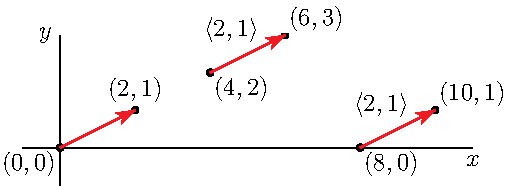
\includegraphics{positions.pdf}
  \end{center}
\end{efig}

By way of summary, 
\begin{notn}\label{not scalar vector}
we use
\begin{itemize}\itemsep1pt \parskip0pt \parsep0pt
\item
bold faced letters, like $\vv$, $\vt$, $\vg$, to designate vectors,
and
\item
angle brackets, like $\llt 2,1\rgt$, around the components of a vector,
but use
\item
round brackets, like $(2,1)$, around the coordinates of a point,
and use
\item ``scalar'' to emphasise that some quantity is a number,
rather than a vector.
\end{itemize}
\end{notn}

%%%%%%%%%%
\subsection{Addition of Vectors and Multiplication of a Vector by a Scalar}
%%%%%%%%%

Just as we have done many times in the CLP texts, when we define a new 
type of object, we want to understand how it interacts with the basic 
operations of addition and multiplication. Vectors are no different, and 
we shall shortly see a natural way to define addition of vectors.
Multiplication will be more subtle, and we shall start with multiplication of a vector by a number (rather than with multiplication of a vector by 
another vector).

By way of motivation for the definitions of addition and multiplication by a number, imagine that we are out for a walk on the $xy$-plane. 
\begin{itemize}
\item 
Suppose that we take a step and, in doing so, we move $a_1$ units parallel to the $x$-axis and $a_2$ units parallel to the $y$-axis. 
Then we say that $\llt a_1, a_2\rgt$ is the displacement vector for the step. Suppose now that we take a second step which moves us an additional $b_1$ units  parallel to the $x$-axis and an additional $b_2$ units  parallel to the $y$-axis, as in the figure on the left below. So the displacement 
vector for the second step is $\llt b_1, b_2\rgt$. All together, we have moved $a_1+b_1$ units  parallel to the $x$-axis and $a_2+b_2$ units parallel to the $y$-axis. The displacement vector for the two steps combined is  
$\llt a_1+b_1, a_2+b_2\rgt$. We shall define
the sum of $\llt a_1, a_2\rgt$ and $\llt b_1, b_2\rgt$, denoted by
$\llt a_1, a_2\rgt+\llt b_1,b_2\rgt$, to be $\llt a_1+b_1, a_2+b_2\rgt$.

\item
Suppose now that, instead, we decide to step in the same direction
as the first step above, but to move twice as far, as in the figure on the right below. That is, our step will move us $2a_1$ units in the direction of the $x$-axis and $2a_2$ units in the direction of the $y$-axis and the 
corresponding displacement vector will be $\llt 2a_1, 2a_2\rgt$. 
We shall define the product of the number $2$ and the vector
$\llt a_1, a_2\rgt$, denoted by $2\llt a_1, a_2\rgt$, to be 
$\llt 2a_1, 2a_2\rgt$.
\end{itemize}

\begin{efig}
  \begin{center}
  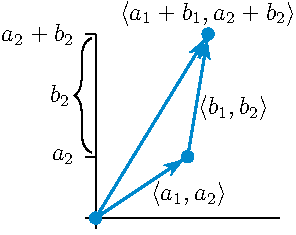
\includegraphics{maddvec.pdf}\qquad
  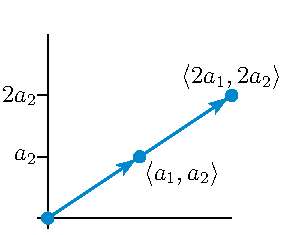
\includegraphics{mscalmul.pdf}
  \end{center}
\end{efig}

Here are the formal definitions.

\begin{defn}[Adding Vectors and Multiplying a Vector by a Number]
             \label{def:addScalMult}
These two operations have the obvious definitions
\begin{alignat*}{2}
&\va=\llt a_1,a_2\rgt,\ \vb =\llt b_1,b_2\rgt
             \qquad&&\implies\qquad\va+\vb=\llt a_1+b_1,a_2+b_2\rgt\\
&\va=\llt a_1,a_2\rgt,\ s\text{ a number}
            \qquad&&\implies\qquad s\va=\llt sa_1,sa_2\rgt
\end{alignat*}
and similarly in three dimensions.
\end{defn} 
Pictorially, you add the vector $\vb$ to the vector $\va$ 
by drawing $\vb$ with its tail at the head of $\va$ and then drawing
a vector from the tail of $\va$ to the head of $\vb$, as in the figure
on the left below. For a number $s$, we can draw the vector $s\va$, by 
just 
\begin{itemize}\itemsep1pt \parskip0pt \parsep0pt
\item
changing the vector $\va$'s length by the factor $|s|$, and,
\item
if $s<0$, reversing the arrow's direction, 
\end{itemize}
as in the other two figures below.
\begin{wfig}
  \begin{center}
  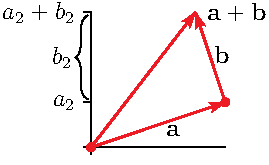
\includegraphics{addvec.pdf}\qquad\qquad
  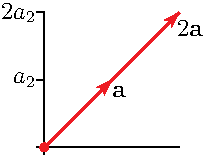
\includegraphics{scalmul.pdf}\qquad\qquad
  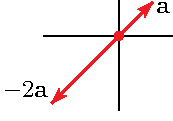
\includegraphics{negmul.pdf}
  \end{center}
\end{wfig}
The special case of multiplication by $s=-1$ appears so frequently that
$(-1)\va$ is given the shorter notation $-\va$. That is, 
\begin{equation*}
-\llt a_1,a_2\rgt=\llt -a_1,-a_2\rgt
\end{equation*}
Of course $\va+(-\va)$ is $\vZero$, the vector all of whose components
are zero. 

To subtract $\vb$ from $\va$ pictorially, 
you may add $-\vb$ (which is drawn by reversing the direction of $\vb$)
 to $\va$. Alternatively,
if you draw $\va$ and $\vb$ with their tails at a common point,
then $\va-\vb$ is the vector from the head of $\vb$ to
the head of $\va$. That is, $\va-\vb$ is the vector you
must add to $\vb$ in order to get $\va$.
\begin{efig}
  \begin{center}
  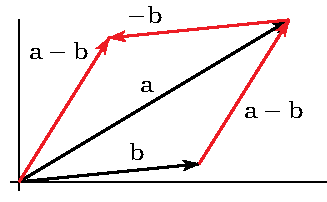
\includegraphics{subtract.pdf}
  \end{center}
\end{efig}


The operations of addition and multiplication by a scalar that we have just
defined are quite natural and rarely cause any problems, because 
they inherit from the real numbers the properties of  addition and 
multiplication that you are used to. 
\begin{theorem}[Properties of Addition and Scalar Multiplication]
                    \label{thm:addScalMult}
Let $\va$, $\vb$ and $\vc$ be vectors and $s$ and $t$ be scalars. Then 
\begin{alignat*}{5}
& (1)\quad&&\va+\vb=\vb+\va \qquad\qquad\qquad
&& (2)\quad&&\va+(\vb+\vc)=(\va+\vb)+\vc\\
& (3) &&\va+\vZero =\va 
&& (4) &&\va+(-\va)=\vZero\\
& (5) &&s(\va+\vb)=s\va+s\vb
&& (6) &&(s+t)\va=s\va+t\va\\
& (7) &&(st)\va = s(t\va)
&& (8) &&1\va=\va\\
\end{alignat*}
\end{theorem}

\noindent We have just been introduced to many definitions. Let's
see some of them in action.
\begin{eg}
For example, if 
\begin{equation*}
\va = \llt 1,2,3\rgt\qquad
\vb = \llt 3,2,1\rgt\qquad
\vc = \llt 1,0,1\rgt
\end{equation*}
then
\begin{alignat*}{3}
2\va&=2\llt 1,2,3\rgt&&=\llt 2,4,6\rgt \\
-\vb&=-\llt 3,2,1\rgt&&=\llt -3,-2,-1\rgt \\
3\vc&=3\llt 1,0,1\rgt&&=\llt 3,0,3\rgt
\end{alignat*}
and 
\begin{align*}
2\va-\vb+3\vc 
&= \llt 2,4,6\rgt + \llt -3,-2,-1\rgt+\llt 3,0,3\rgt \\
&= \llt 2-3+3\,,\,4-2+0\,,\,6-1+3\rgt \\
&= \llt 2,2,8 \rgt
\end{align*}
\end{eg}\goodbreak

\begin{defn}\label{def parallel vectors}
Two vectors $\va$ and $\vb$
\begin{itemize}
\item
are said to be parallel if $\ \va= s\,\vb\ $ for some nonzero real number $s$ and
\item
are said to have the same direction if $\ \va=s\,\vb\ $ for some number $s>0$.
\end{itemize} 
\end{defn}


There are some vectors that occur sufficiently commonly that they are
given special names. One is the vector $\vZero$. Some others are the 
``standard basis vectors''.
\begin{defn}\label{def basis vectors}
\begin{enumerate}[(a)]
\item
The standard basis vectors in two dimensions are
\begin{align*}
\\[-0.1in]
\hi = \llt 1,0\rgt \qquad\qquad\hj =\llt 0,1\rgt \qquad\qquad
\smash{\raisebox{-0.5\height}{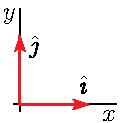
\includegraphics{basis2d.pdf}}}\\[-0.1in]
\end{align*} 
\item
The standard basis vectors in three dimensions are
\begin{align*}
\\[-0.1in]
\hi = \llt 1,0,0\rgt \qquad\qquad\hj =\llt 0,1,0\rgt 
\qquad\qquad\hk =\llt 0,0,1\rgt \qquad\quad
\smash{\raisebox{-0.25\height}{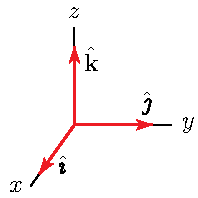
\includegraphics{basis3d.pdf}}}\\[-0.1in]
\end{align*}
\end{enumerate} 
\end{defn}
We'll explain the little hats in the notation $\hi$, $\hj$, $\hk$ shortly.
Some people rename $\hi$, $\hj$ and $\hk$ to $\he_1$, $\he_2$ and 
$\he_3$ respectively.
Using the above properties we have, for all vectors,
\begin{equation*}
\llt a_1,a_2\rgt =a_1\,\hi+a_2\,\hj\qquad\qquad
\llt a_1,a_2,a_3\rgt =a_1\,\hi+a_2\,\hj+a_3\,\hk
\end{equation*}
A sum of numbers times vectors, like $a_1\hi+a_2\hj$ is called
a linear combination of the vectors.
Thus all vectors can be expressed as linear combinations of the standard
basis vectors. This makes basis vectors very helpful in computations.
The  standard basis vectors are unit vectors, meaning that they are of 
length one, where the length of a vector $\va$ is denoted\footnote{The notation $\|\va\|$ is also used for the length of $\va$.} $|\va|$ 
and is defined by
\begin{defn}[Length of a Vector]\label{def:vectLen}
\begin{alignat*}{5}
&\va=\llt a_1,a_2\rgt \qquad&&\implies\qquad &&|\va|=\sqrt{a_1^2+a_2^2}\\
&\va=\llt a_1,a_2,a_3\rgt \qquad&&\implies\qquad &&|\va|=\sqrt{a_1^2+a_2^2+a_3^2}
\end{alignat*}
A unit vector is a vector of length one. We'll sometimes use the accent 
$\hat{\ }$ to emphasise that the vector $\hat\va$ is a unit vector.
That is, $|\hat\va|=1$.
\end{defn}


\begin{eg}\label{eg unit vector}
Recall that multiplying a vector $\va$ by a positive number $s$,
changes the length of the vector by a factor $s$ without changing
the direction of the vector. So (assuming that $|\va|\ne 0)$
$\frac{\va}{|\va|}$ is a unit vector that has the same direction as
$\va$. For example, $\frac{\llt 1,1,1\rgt}{\sqrt{3}}$ is a unit vector
that points in the same direction as $\llt 1,1,1\rgt$.
\end{eg}
\goodbreak

\begin{eg}\label{eg walk}
We go for a walk on a flat Earth. We use a coordinate system
with the positive x-axis pointing due east and the positive y-axis pointing due
north. We  
\begin{itemize}\itemsep1pt \parskip0pt \parsep0pt
\item
start at the origin and
\item 
walk due east for 4 units and then
\item 
walk northeast for $5\sqrt{2}$ units and then
\item 
head towards the point $(0,11)$, but we only go
\item
one third of the way.
\end{itemize}
      \begin{efig} 
      \begin{center}
      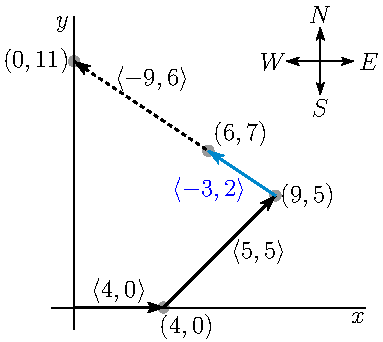
\includegraphics{addSubtractMult.pdf}\qquad\qquad
      \raisebox{0.65\height}{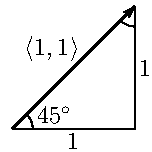
\includegraphics{triangleWalk.pdf}}
      \end{center}
      \end{efig}
We will now use vectors to figure out our final location.
\begin{itemize}\itemsep1pt \parskip0pt \parsep0pt
\item
On the first leg of our walk, we go 4 units in the positive $x$-direction.
So our displacement vector --- the vector whose tail is at our starting point and whose head is at the end point of the first leg --- is $\llt 4,0\rgt$. 
As we started at $(0,0)$ we finish the first leg of the walk at $(4,0)$.
\item
On the second leg of our walk, our direction of motion is northeast, i.e. is
$45^\circ$ above the direction of the positive $x$-axis. Looking at the figure 
on the right above, we see that our displacement vector, for the second leg of the walk, has to be in the same direction as the vector $\llt 1,1\rgt$.
So our displacement vector is the vector of length $5\sqrt{2}$ with the same direction as $\llt 1,1\rgt$. The vector $\llt 1,1\rgt$ has length
$\sqrt{1^2+1^2}=\sqrt{2}$ and so $\frac{\llt 1,1\rgt}{\sqrt{2}}$ has length one
and our displacement vector is
\begin{equation*}
5\sqrt{2}\ \frac{\llt 1,1\rgt}{\sqrt{2}}
=5 \llt 1,1\rgt 
=\llt 5,5\rgt
\end{equation*}
If we draw this displacement vector, $\llt 5,5\rgt$ with its tail at 
$(4,0)$, the starting point of the second leg of the walk, then its head 
will be at $(4+5, 0+5)=(9,5)$ and that is the end point of the second 
leg of the walk.
\item
On the final leg of our walk, we start at $(9,5)$ and walk towards $(0,11)$.
The vector from $(9,5)$ to $(0,11)$ is $\llt 0-9\,,\,11-5\rgt =\llt -9,6\rgt$.
As we go only one third of the way, our final displacement vector is
\begin{equation*}
\frac{1}{3}\llt -9,6\rgt
=\llt -3,2\rgt
\end{equation*}
If we draw this displacement vector with its tail at 
$(9,5)$, the starting point of the final leg, then its head 
will be at $(9-3, 5+2)=(6,7)$ and that is the end point of the final
leg of the walk, and our final location.
\end{itemize}
\end{eg}

%%%%%%%%%%%%%%%%%%%%%%%%%%%%%%%%%%%%%%%%%%%%%%%%%%%%%%%%%%%
\subsection{The Dot Product}\label{subsec dot product}
%%%%%%%%%%%%%%%%%%%%%%%%%%%%%%%%%%%%%%%%%%%%%%%%%%%%%%%%%%%
Let's get back to the arithmetic operations of addition and multiplication.
We will be using both scalars and vectors. So, for each operation there are 
three possibilities that we need to explore: 
\begin{itemize}\itemsep1pt \parskip0pt \parsep0pt
\item ``scalar plus scalar'', ``scalar plus vector'' and ``vector plus vector''
\item``scalar times scalar'', ``scalar times vector'' and 
         ``vector times vector''
\end{itemize}
We have been using ``scalar plus scalar'' and ``scalar times scalar''
since childhood. ``vector plus vector'' and ``scalar times vector''
were just defined above. There is no sensible way to define ``scalar plus vector'', so we won't. This leaves ``vector times vector''. 
There are actually two widely used such products.
The first is the \emph{dot product}, which is the topic of this section,
and which is used to easily determine the angle $\theta$ (or more precisely,
$\cos\theta$) between two vectors.
We'll get to the second, the cross product, later. 

Here is preview of what we will do in this dot product 
subsection \S\ref{subsec dot product}. We are going to give two formulae
for the dot product, $\va\cdot\vb$, of the pair of vectors 
$\va=\llt a_1,a_2,a_3\rgt$ and $\vb=\llt b_1,b_2,b_3\rgt$.
\begin{itemize}
\item 
The first formula is $\va\cdot\vb = a_1b_1+a_2b_2+a_3b_3$.
We will take it as our official definition of $\va\cdot\vb$.
This formula provides us with an easy way to compute dot products.

\item
The second formula is $\va\cdot\vb=|\va|\,|\vb|\,\cos\theta$, 
        where $\theta$ is the angle between $\va$ and $\vb$.
      \begin{efig} 
      \begin{center}
      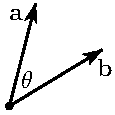
\includegraphics{dotAngle.pdf}
      \end{center}
      \end{efig}
We will show, in Theorem \ref{thm:dotPppties} below, that this second formula always gives the same answer as the first formula.
The second formula provides us with an easy way to determine the angle between two vectors. In particular, it provides us with an easy way to test whether or not two vectors are perpendicular to each other. For example,
the vectors $\llt 1,2,3\rgt$ and $\llt -1,-1,1\rgt$ have dot product
\begin{equation*}
\llt 1,2,3\rgt\cdot\llt -1,-1,1\rgt = 1\times(-1)+2\times(-1)+3\times 1=0
\end{equation*}
This tell us as the angle $\theta$ between the two vectors obeys 
$\cos\theta=0$, so that $\theta=\frac{\pi}{2}$. That is, the two vectors are perpendicular to each other.
\end{itemize}
After we give our official definition of the dot product in
Definition \ref{def:dotProd}, and give the important properties of the dot product, including the formula  $\va\cdot\vb=|\va|\,|\vb|\,\cos\theta$,
in Theorem \ref{thm:dotPppties}, we'll give some examples.
Finally, to see the dot product in action, we'll define what it means to 
project one vector on another vector and give an example.

\begin{defn}[Dot Product]\label{def:dotProd}
The dot product of the vectors $\va$ and $\vb$ is denoted $\va\cdot\vb$ 
and is defined by
\begin{alignat*}{5}
&\va=\llt a_1,a_2\rgt ,\quad &&\vb=\llt b_1,b_2\rgt\quad &\implies\quad
&\va\cdot\vb = a_1b_1+a_2b_2\\
&\va=\llt a_1,a_2,a_3\rgt ,\quad &&\vb=\llt b_1,b_2,b_3\rgt\quad &\implies\quad
&\va\cdot\vb = a_1b_1+a_2b_2+a_3b_3
\end{alignat*}
in two and three dimensions respectively. 
\end{defn}
The properties of the dot 
product are as follows:
\begin{theorem}[Properties of the Dot Product]\label{thm:dotPppties}
Let $\va$, $\vb$ and $\vc$ be vectors and let $s$ be a scalar. Then
\begin{alignat*}{3}
&(0)\quad &&\va,\vb\text{ are vectors and }\va\cdot\vb
              \text{ is a scalar}\\
&(1) &&\va\cdot\va=|\va|^2\\
&(2) &&\va\cdot\vb=\vb\cdot\va\\
&(3) &&\va\cdot(\vb+\vc)=\va\cdot\vb+\va\cdot\vc,\quad 
       (\va+\vb)\cdot\vc=\va\cdot\vc+\vb\cdot\vc\\
&(4) &&(s\va)\cdot\vb= s(\va\cdot\vb)\\
&(5)  &&\vZero \cdot\va=0\\
&(6) &&\va\cdot\vb=|\va|\,|\vb|\,\cos\theta
        \text{ where $\theta$ is the angle between $\va$ and $\vb$}\\
&(7) &&\va\cdot\vb=0\iff \va=\vZero \text{ or }\vb=\vZero 
    \text{ or } \va\perp\vb
\end{alignat*}
\end{theorem}
\begin{proof}
Properties 0 through 5 are almost immediate consequences of the definition.
For example, for property 3 (which is called the distributive law)
in dimension 2,
\begin{align*}
\va\cdot(\vb+\vc)
    &=\llt a_1,a_2\rgt \cdot\llt b_1+c_1,b_2+c_2\rgt \\
    &=a_1(b_1+c_1)+a_2(b_2+c_2)=a_1b_1+a_1c_1+a_2b_2+a_2c_2\\
\va\cdot\vb+\va\cdot\vc
&=\llt a_1,a_2\rgt \cdot\llt b_1,b_2\rgt 
             +\llt a_1,a_2\rgt \cdot\llt c_1,c_2\rgt \\
&=a_1b_1+a_2b_2+a_1c_1+a_2c_2
\end{align*}


Property 6 is sufficiently important that it is often used as the 
definition of dot product. It is not at all an obvious consequence of the definition.
To verify it, we just write $|\va-\vb|^2$ in two different ways. 
The first expresses $|\va-\vb|^2$ in terms of $\va\cdot\vb$. 
It is
\begin{align*}
|\va-\vb|^2\ &{\buildrel 1 \over =}\ (\va-\vb\,)\cdot(\va-\vb\,)\\
&{\buildrel 3 \over =}\ \va\cdot\va-\va\cdot\vb-\vb\cdot\va
+\vb\cdot\vb\\
&{\buildrel 1,2 \over =}\ |\va|^2+|\vb|^2-2\va\cdot\vb
\end{align*}
Here, ${\buildrel 1 \over =}$, for
example, means that the equality is  a consequence of property 1.
The second way we write $|\va-\vb|^2$ involves $\cos\theta$ and follows from
the cosine law for triangles. Just in case you don't remember the 
cosine law, we'll derive it right now! Start by applying Pythagoras to the 
shaded triangle in the right hand figure of

      \begin{efig} 
      \begin{center}
      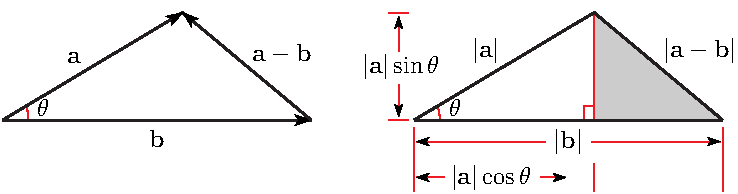
\includegraphics{cosineB.pdf}
      \end{center}
      \end{efig}
That triangle is a right triangle whose hypotenuse has length $|\va-\vb|$ 
and  whose other two sides have lengths $\big(|\vb|-|\va|\cos\theta\big)$ 
and $|\va|\sin\theta$. So Pythagoras gives
\begin{align*}
|\va-\vb|^2&=\big(|\vb|-|\va|\cos\theta\big)^2+
\big(|\va|\sin\theta\big)^2\\
&=|\vb|^2-2|\va|\,|\vb|\,\cos\theta+|\va|^2\cos^2\theta
+|\va|^2\sin^2\theta\\
&=|\vb|^2-2|\va|\,|\vb|\,\cos\theta+|\va|^2
\end{align*}
This is precisely the cosine law\footnote{You may be used to seeing it written as $c^2=a^2+b^2-2 a b \cos C$, where $a$, $b$ and $c$ are the lengths of the 
three sides of the triangle and $C$ is the angle opposite the side of length $c$}. 
Observe that, when $\theta=\tfrac{\pi}{2}$, 
this reduces to, (surprise!) Pythagoras' theorem.

Setting our two expressions for $|\va-\vb|^2$ equal to each other,
\begin{align*}
|\va-\vb|^2=|\va|^2+|\vb|^2-2\va\cdot\vb
=|\vb|^2-2|\va|\,|\vb|\,\cos\theta+|\va|^2
\end{align*}
cancelling the $|\va|^2$ and $|\vb|^2$ common to both sides
\begin{align*}
-2\va\cdot\vb
=-2|\va|\,|\vb|\,\cos\theta
\end{align*}
and dividing by $-2$ gives 
\begin{align*}
\va\cdot\vb=|\va|\,|\vb|\,\cos\theta
\end{align*}
which is exactly property 6. 


Property 7 follows directly from property 6. First note that the dot product $\va\cdot\vb=|\va|\,|\vb|\,\cos\theta$
is zero if and only if at least one of the three factors 
$|\va|,\ |\vb|,\ \cos\theta$ is zero. The first factor is zero if
and only if $\va=\vZero $. The second factor is zero if and only if 
$\vb=\vZero $.
The third factor is zero if and only if $\theta=\pm\tfrac{\pi}{2}+2k\pi$,
for some integer $k$, which in turn is true if and only if $\va$ and 
$\vb$ are mutually perpendicular.
\end{proof}
Because of Property 7 of Theorem \ref{thm:dotPppties}, the dot product 
can be used to test whether or not two vectors are perpendicular to 
each other. That is, whether or not the angle between the two vectors 
is $90^\circ$. Another name\footnote{The concepts of the dot product
and perpendicularity have been generalized a lot in mathematics (for example,
from 2d and 3d vectors to functions). The generalization of the dot 
product is called the ``inner product'' and the generalization 
of perpendicularity is called ``orthogonality''.} for ``perpendicular'' 
is ``orthogonal''. Testing for orthogonality is one of the main uses of the
dot product. 

\begin{eg}
Consider the three vectors
\begin{equation*}
\va=\llt 1,1,0 \rgt\qquad
\vb=\llt 1,0,1 \rgt \qquad
\vc=\llt -1,1,1\rgt
\end{equation*}
Their dot products
\begin{alignat*}{3}
\va\cdot\vb & = \llt 1,1,0 \rgt \cdot \llt 1,0,1 \rgt
           && = 1\times 1 +1\times 0+0\times 1
           && = 1 \\
\va\cdot\vc & = \llt 1,1,0 \rgt \cdot \llt -1,1,1 \rgt
           && = 1\times(-1) +1\times 1+0\times 1
           && = 0 \\
\vb\cdot\vc & = \llt 1,0,1 \rgt \cdot \llt -1,1,1 \rgt
           && = 1\times(-1) +0\times 1+1\times 1
           && = 0
\end{alignat*}
tell us that $\vc$ is perpendicular to both $\va$ and $\vb$.
Since both $|\va|=|\vb|=\sqrt{1^2+1^2+0^2}=\sqrt{2}$ the first dot product
tells us that the angle, $\theta$, between $\va$ and $\vb$ obeys
\begin{align*}
\cos\theta =\frac{\va\cdot\vb}{|\va|\,|\vb|}=\frac{1}{2}
\implies
\theta =\frac{\pi}{3}
\end{align*}

\begin{efig}
  \begin{center}
  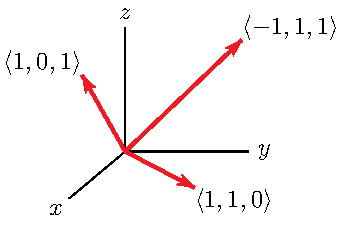
\includegraphics{dotProd.pdf}
  \end{center}
\end{efig}

\end{eg}
\goodbreak


Dot products are also used to compute projections.  First, here's
the definition.

\begin{defn}[Projection]\label{def:projection}
Draw two vectors, $\va$ and $\vb$,
with their tails at a common point and drop a perpendicular from the head of
$\va$ to the line that passes through both the head and tail of $\vb$. 
By definition, the projection of the vector $\va$
on the vector $\vb$ is the vector from the tail of $\vb$ to the point
on the line where the perpendicular hits.
      \begin{efig} 
      \begin{center}
      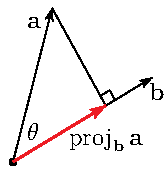
\includegraphics{projA.pdf}\qquad\qquad
      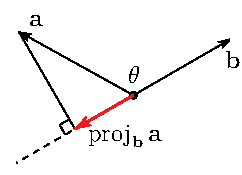
\includegraphics{projB.pdf}
      \end{center}
      \end{efig}
\end{defn}\noindent
Think of the projection of $\va$ on $\vb$ as the part of $\va$ that is in the 
direction of $\vb$.

Now let's develop a formula for the projection of $\va$ on $\vb$.
Denote by $\theta$ the angle between $\va$ and $\vb$. If $|\theta|$ is no
more than $90^\circ$, as in the figure on the left above, 
the length of the projection of $\va$ on $\vb$ is 
$|\va|\cos\theta$.
By Property 6 of Theorem \ref{thm:dotPppties},  
$|\va|\cos\theta=\va\cdot\vb/|\vb|$, so the
projection is a vector whose length is $\va\cdot\vb/|\vb|$ and
whose direction is given by the unit vector $\vb/|\vb|$. Hence
\begin{align*}
\text{projection of $\va$ on $\vb$}={\rm proj}_{\vb}\,\va
=\frac{\va\cdot\vb}{|\vb|}\frac{\vb}{|\vb|}
=\frac{\va\cdot\vb}{|\vb|^2}\,\vb
\end{align*}
If $|\theta|$ is larger than $90^\circ$, as in the figure on the right above, the projection has length 
$|\va|\,\cos(\pi-\theta)=-|\va|\cos\theta=-\va\cdot\vb/|\vb|$
 and direction $-\vb/|\vb|$. In this case
\begin{align*}
{\rm proj}_{\vb}\,\va
=-\frac{\va\cdot\vb}{|\vb|}\ \frac{-\vb}{|\vb|}
=\frac{\va\cdot\vb}{|\vb|^2}\ \vb
\end{align*}
So the formula 
\begin{impeqn}\label{eqn proj}
\begin{equation*}
{\rm proj}_{\vb}\,\va=\frac{\va\cdot\vb}{|\vb|^2}\,\vb
\end{equation*} 
\end{impeqn}\noindent
is applicable whenever $\vb\ne\vZero $. As a special case, if $\vb$ happens 
to be a unit vector, which, for emphasis, we'll now write has $\hat\vb$, 
the projection formula simplifies to
\begin{impeqn}\label{eqn unit proj}
\begin{align*}
{\rm proj}_{\hat\vb}\,\va
=  (\va\cdot\hat\vb)\,\hat\vb
\end{align*}
\end{impeqn}

\begin{eg}\label{eg proj}
In this example, we will find the projection of the vector $\llt 0,3\rgt$
on the vector $\llt 1,1\rgt$, as in the figure
      \begin{efig} 
      \begin{center}
      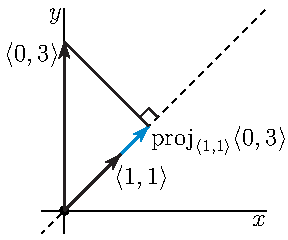
\includegraphics{projEg.pdf}
      \end{center}
      \end{efig}
By Equation \ref{eqn proj} with $\va=\llt 0,3\rgt$ and $\vb=\llt 1,1\rgt$, 
that projection is
\begin{align*}
{\rm proj}_{\llt 1,1\rgt}\,\llt 0,3\rgt
  &=\frac{\llt 0,3\rgt\cdot\llt 1,1\rgt}{|\llt 1,1\rgt|^2}\,\llt 1,1\rgt \\
  &=\frac{0\times1+3\times 1}{1^2+1^2}\,\llt 1,1\rgt
  =\llt \frac{3}{2},\frac{3}{2}\rgt
\end{align*}

\end{eg}

One use of projections is to ``resolve forces''. There is an example in
the next (optional) section.

%%%%%%%%%%%%%%%%%%%%%%%%%%%%%%%%%%%%%%%%%%%%%%%%%%%%%%%%%%%%%%%%%%%%
\subsection{(Optional) Using Dot Products to Resolve Forces
--- The Pendulum}
%%%%%%%%%%%%%%%%%%%%%%%%%%%%%%%%%%%%%%%%%%%%%%%%%%%%%%%%%%%%%%%%%%%%
Model a pendulum by a mass $m$ that is connected to a hinge by an idealized
rod that is massless and of fixed length $\ell$. Denote by $\theta$ the angle
between the rod and vertical. The forces acting on the mass are
\begin{itemize}
\item gravity, which has magnitude $mg$ and direction $\llt 0,-1\rgt$, 
\item tension in the rod, whose magnitude $\tau(t)$ automatically 
adjusts itself so that the distance between the mass and the hinge is fixed 
at $\ell$ (so that the rod does not stretch or contract) and whose 
direction is always parallel to the rod, 
\item and possibly some frictional
forces, like friction in the hinge and air resistance. Assume
that the total frictional force has magnitude proportional\footnote{The
behaviour of air resistance (sometimes called drag) is pretty complicated. 
We're using a reasonable low speed approximation. At high speeds drag is typically proportional to the square of the speed.} to the speed of the 
mass and has direction opposite to the direction of motion of the mass.
We'll call the constant of proportionality $\beta$.
\end{itemize}
      \begin{efig} 
      \begin{center}
      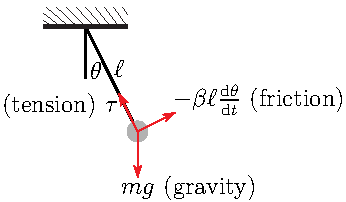
\includegraphics{pendulum3.pdf}
      \end{center}
      \end{efig}
If we use a coordinate system centered on the hinge, the $(x,y)$ coordinates
of the mass at time $t$ are 
\begin{align*}
x(t)&=\ell\sin\theta(t)\\
y(t)&=-\ell\cos\theta(t)
\end{align*}
where $\theta(t)$ is the angle between the rod and vertical at time $t$.
We are now going to use Newton's law of motion
\begin{align*}
\text{mass}\times\text{acceleration}=\text{total applied force}
\end{align*}
to determine now $\theta$ evolves in time. By definition, the
velocity and acceleration vectors\footnote{For a more comprehensive treatment 
of derivatives of vector valued functions $\vr(t)$, and in particular of
velocity and acceleration, see Section \ref{sec curves} in this text and
Section 1.1 in the CLP-4 text.} for the position vector 
$\llt x(t),y(t)\rgt$ are
\begin{align*}
\diff{}{t}\llt x(t),y(t)\rgt 
   &= \llt \diff{x}{t}(t),\diff{y}{t}(t)\rgt \\
\ddiff{2}{}{t}\llt x(t),y(t)\rgt 
   &=\llt \ddiff{2}{x}{t}(t),\ddiff{2}{y}{t}(t)\rgt 
\end{align*}
So, the velocity and acceleration vectors of our mass are
\begin{alignat*}{3}
\vv(t)&=\diff{}{t}\llt x(t),y(t)\rgt 
&&=\llt \ell\diff{}{t}\sin\theta(t),-\ell\diff{}{t}\cos\theta(t)\rgt \\
&=\llt \ell\cos\theta(t)\,\diff{\theta}{t}(t)\,,\,
             \ell\sin\theta(t)\,\diff{\theta}{t}(t)\rgt\hidewidth \\
&=\ell\,\diff{\theta}{t}(t)\,\llt \cos\theta(t),\sin\theta(t)\rgt \hidewidth
  \\[0.1in]
\va(t)&=\ddiff{2}{}{t}\llt x(t),y(t)\rgt 
&&=\diff{}{t}
  \left\{\ell\,\diff{\theta}{t}(t)\,
               \llt \cos\theta(t),\sin\theta(t)\rgt \right\} \\ 
&=\ell\,\ddiff{2}{\theta}{t}(t)\,\llt \cos\theta(t),\sin\theta(t)\rgt 
+\ell\,\diff{\theta}{t}(t)
       \llt \diff{}{t}\cos\theta(t),\diff{}{t}\sin\theta(t)\rgt \,\hidewidth\\
&= \ell\,\ddiff{2}{\theta}{t}(t)\llt \cos\theta(t),\sin\theta(t)\rgt 
+\ell \Big(\diff{\theta}{t}(t)\Big)^2
     \llt -\sin\theta(t),\cos\theta(t)\rgt\hidewidth
\end{alignat*}

The negative of the velocity vector is  
$- \ell\, \diff{\theta}{t}\llt \cos\theta,\sin\theta\rgt$, so the total frictional force is 
\begin{equation*}
-\beta\ell\, \diff{\theta}{t}\llt \cos\theta,\sin\theta\rgt 
\end{equation*} 
with $\beta$ our constant of proportionality. 

The vector 
\begin{equation*}
\tau(t) \llt -\sin\theta(t),\cos\theta(t)\rgt 
\end{equation*}
has magnitude $\tau(t)$ and direction parallel to the rod pointing 
from the mass towards the hinge and so is the force due to tension 
in the rod. 

Hence, for this physical system, Newton's law of motion is 
\begin{align}
&\overbrace{m\ell\,\ddiff{2}{\theta}{t}\llt \cos\theta,\sin\theta\rgt 
+m\ell\,\Big(\diff{\theta}{t}\Big)^2\llt -\sin\theta,\cos\theta\rgt}^
        {\text{mass}\times\text{acceleration}}
  \notag\\
&\hskip1in=
\overbrace{mg\llt 0,-1\rgt}^{\rm gravity} 
 +\overbrace{\tau \llt -\sin\theta,\cos\theta\rgt}^{\rm tension}
-\overbrace{\beta\ell\,\diff{\theta}{t}\llt \cos\theta,\sin\theta\rgt}^{\rm friction} 
\tag{$*$}
\end{align}
This is a rather complicated looking equation. Writing out its $x$- and
$y$-components doesn't help. They also look complicated.
Instead, the equation can be considerably simplified (and 
consequently better understood) by ``taking its components parallel to
and perpendicular to the direction of motion''. From the velocity vector
$\vv(t)$, we see that $\llt \cos\theta(t),\sin\theta(t)\rgt $ is a unit 
vector parallel to the direction of motion at time $t$.
Recall, from \eqref{eqn unit proj}, that the projection of any vector 
$\vb$ on any unit vector $\hat\vd$ 
(with the ``hat'' on $\hat\vd$ reminding ourselves that the vector is a unit
vector) is
\begin{align*}
%\frac{\vb\cdot\hat\vd}{{|\hat\vd|}^2}\,\hat\vd  =
\big(\vb\cdot \hat\vd\big)\,\hat\vd
\end{align*}
The coefficient $\vb\cdot \hat\vd$ is, by definition, the
component of $\vb$ in the direction $\hat\vd$.
So, by dotting both sides of the equation of motion $(*)$ with
$\hat\vd=\llt \cos\theta(t),\sin\theta(t)\rgt $, we extract the component 
parallel to the direction of motion. Since
\begin{align*}
\llt \cos\theta,\sin\theta\rgt \cdot\llt \cos\theta,\sin\theta\rgt &=1\\
\llt \cos\theta,\sin\theta\rgt \cdot\llt -\sin\theta,\cos\theta\rgt &=0\\
\llt \cos\theta,\sin\theta\rgt \cdot\llt 0,-1\rgt &=-\sin\theta
\end{align*}
this gives
\begin{align*} 
m\ell\ddiff{2}{\theta}{t}=-mg\sin\theta-\beta\ell\diff{\theta}{t}
\end{align*}
which is \emph{much} cleaner than $(*)$!
When $\theta$ is small, we can approximate $\sin\theta\approx\theta$ 
and get the equation
\begin{align*}
\ddiff{2}{\theta}{t}+\frac{\beta}{m}\diff{\theta}{t}+\frac{g}{\ell}\theta=0
\end{align*}
which is easily solved. There are systematic procedures for finding 
the solution, but we'll just guess. 

When there is no friction (so that $\beta=0$),
we would expect the pendulum to just oscillate. So it is natural to guess
\begin{equation*}
\theta(t)=A\sin(\omega t-\delta)
\end{equation*}
which is an oscillation with (unknown) amplitude $A$, 
frequency $\omega$ (radians per unit time) and 
phase $\delta$. Substituting this guess into the left hand side, 
$\theta''+\tfrac{g}{\ell}\theta$,  yields 
\begin{equation*}
-A\omega^2\sin(\omega t-\delta)+A\tfrac{g}{\ell}\sin(\omega t-\delta)
\end{equation*} 
which is zero if $\omega=\sqrt{g/\ell}$. So
$\ \theta(t)=A\sin(\omega t-\delta)\ $ is a solution for any amplitude 
$A$ and phase $\delta$, provided the frequency $\omega=\sqrt{g/\ell}$. 

When there is some, but not too much, friction, so that $\beta>0$ is 
relatively small, we would expect ``oscillation with decaying amplitude''. 
So we  guess 
\begin{equation*}
\theta(t)=Ae^{-\gamma t}\sin(\omega t-\delta)
\end{equation*}
for some constant decay rate $\gamma$, to be determined.
With this guess,
\begin{alignat*}{3}
\theta(t)&=\phantom{- -\gamma\omega^{2})} Ae^{-\gamma t}
                   &\sin(\omega t-\delta)\\
\theta'(t)&=\phantom{-\omega^{2})}-\gamma Ae^{-\gamma t}
                  &\sin(\omega t-\delta)
&+\phantom{2\gamma }\omega A e^{-\gamma t}&\cos(\omega t-\delta)\\
\theta''(t)&=(\gamma^2-\omega^2)Ae^{-\gamma t}&\sin(\omega t-\delta)
                    &-2\gamma\omega A e^{-\gamma t}&\cos(\omega t-\delta)
\end{alignat*}
and the left hand side
\begin{align*}
&\ddiff{2}{\theta}{t}+\frac{\beta}{m}\diff{\theta}{t}+\frac{g}{\ell}\theta
 \\
&\hskip0.5in
=\left[\gamma^2-\omega^2-\frac{\beta}{m}\gamma+\frac{g}{\ell}\right] 
                         Ae^{-\gamma t}\sin(\omega t-\delta)
+\left[-2\gamma\omega+\frac{\beta}{m}\omega\right] 
                         Ae^{-\gamma t}\cos(\omega t-\delta)
\end{align*}
vanishes if $\gamma^2-\omega^2-\frac{\beta}{m}\gamma+\tfrac{g}{\ell}=0$ and 
$-2\gamma\omega+\frac{\beta}{m}\omega=0.$ The second equation tells us the decay
rate $\gamma=\tfrac{\beta}{2m}$ and then the first tells us the frequency
\begin{align*}
\omega=\sqrt{\gamma^2-\tfrac{\beta}{m}\gamma+\tfrac{g}{\ell}}
=\sqrt{\tfrac{g}{\ell}-\tfrac{\beta^2}{4m^2}}
\end{align*} 
When there is a lot of friction
(namely when $\tfrac{\beta^2}{4m^2}>\tfrac{g}{\ell}$, so that the frequency
$\omega$ is not a real number), we would expect damping without oscillation 
and so would guess $\theta(t)=Ae^{-\gamma t}$. You can determine the allowed
values of $\gamma$ by substituting this guess in. 


To extract the components perpendicular to the direction of motion, we
dot with $\llt -\sin\theta,\cos\theta\rgt $ rather than $\llt \cos\theta,\sin\theta\rgt $. Note that,
because $\llt -\sin\theta,\cos\theta\rgt \cdot
   \llt \cos\theta,\sin\theta\rgt =0$, the vector
$\llt -\sin\theta,\cos\theta\rgt $ really is perpendicular to the 
direction of motion.  Since
\begin{align*}
\llt -\sin\theta,\cos\theta\rgt \cdot\llt \cos\theta,\sin\theta\rgt &=0\\
\llt -\sin\theta,\cos\theta\rgt \cdot\llt -\sin\theta,cos\theta\rgt &=1\\
\llt -\sin\theta,\cos\theta\rgt \cdot\llt 0,-1\rgt &=-\cos\theta
\end{align*}
dotting both sides of the equation of motion $(*)$
with $\llt -\sin\theta,\cos\theta\rgt $ gives
\begin{align*}
m\ell\Big(\diff{\theta}{t}\Big)^2=-mg\cos\theta+\tau 
\end{align*}
This equation just determines the tension
$\tau=m\ell\big(\diff{\theta}{t}\big)^2+mg\cos\theta$ in the rod, once you know
$\theta(t)$.

%%%%%%%%%%%%%%%%%%%%%%%%%%%%%%%%%%%%%%%%%%%%%%%%%%%%%%%%%%%%%%
\subsection{(Optional) Areas of Parallelograms}\label{sec:GEOparallelogram}
%%%%%%%%%%%%%%%%%%%%%%%%%%%%%%%%%%%%%%%%%%%%%%%%%%%%%%%%%%%%%%
A parallelogram is naturally determined by the two vectors that 
define its sides. We'll now develop a formula for the area of a
parallelogram in terms of these two vectors. 

Construct a parallelogram as follows. Pick two vectors $\llt a,b\rgt $ 
and $\llt c,d\rgt $. Draw them with their tails at a common point. Then 
draw $\llt a,b\rgt $ a second time with its tail at the head of 
$\llt c,d\rgt $ and draw  $\llt c,d\rgt $ a second time with its tail 
at the head of $\llt a,b\rgt $. If the common point is the
origin, you get a picture like the figure below.
\vadjust{
      \begin{efig} 
      \begin{center}
      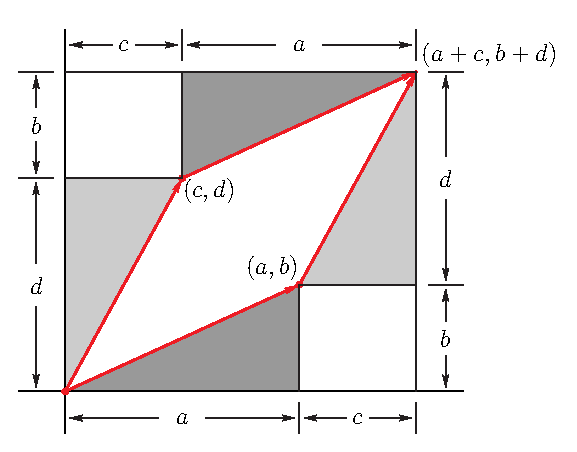
\includegraphics{area3}
      \end{center}
      \end{efig}
        }%
Any parallelogram can be constructed like this if you pick the common point
and two vectors appropriately. Let's compute the area of the parallelogram.
The area of the large rectangle with vertices $(0,0),\ (0, b+d),\ (a+c,0)$
and $(a+c,b+d)$ is $(a+c)(b+d)$. The parallelogram we want can be extracted
from the large rectangle by deleting the two small rectangles (each of
area $bc$), and the two lightly shaded triangles (each of area $\half cd$),
and the two darkly shaded triangles (each of area $\half ab$). So the desired
\begin{align*}
{\rm area} = (a+c)(b+d) - (2\times bc) -\big(2\times \half cd\big)
 -\big(2\times\half ab\big)
=ad-bc
\end{align*}
In the above figure, we have implicitly assumed that $a,\ b,\ c,\ d\ge 0$
and $d/c\ge b/a$. In words, we have assumed that both vectors 
$\llt a,b\rgt ,\ \llt c,d\rgt $ lie in the first quadrant and that 
$\llt c,d\rgt $ lies above $\llt a,b\rgt $.
By simply interchanging $a\leftrightarrow c$ and $b\leftrightarrow d$
in the picture and throughout the argument, we see that when 
$a,\ b,\ c,\ d\ge 0$ and $b/a\ge d/c$, so that the vector $\llt c,d\rgt $ 
lies below $\llt a,b\rgt $, the area of the parallelogram is $bc-ad$. 
In fact, all cases are covered by the formula
\begin{impeqn}\label{eq pgram area}
\begin{align*}
\text{area of parallelogram with sides $\llt a,b\rgt $ and $\llt c,d\rgt =|ad-bc|$}
\end{align*}
\end{impeqn}

Given two vectors $\llt a,b\rgt $ and $\llt c,d\rgt $, the expression 
$ad-bc$ is generally written
\begin{align*}
\det\left[\begin{matrix}a&b\\ c&d\end{matrix}\right]=ad-bc
\end{align*}
and is called the \emph{determinant} of the matrix\footnote{The topics of
matrices and determinants appear prominently in linear algebra courses. We
are only going to use them as notation, and we will explicitly explain
that notation. A linear algebra course is \emph{not} a prerequisite 
for this text.} 
\begin{align*}
\left[\begin{matrix}a&b\\ c&d\end{matrix}\right]
\end{align*} 
with rows $\llt a,b\rgt $ and $\llt c,d\rgt $. The determinant
of a $2\times 2$ matrix is the product of the diagonal entries 
minus the product of the off-diagonal entries. 


There is a similar formula in three dimensions. Any three vectors 
$\va=\llt a_1,a_2,a_3\rgt ,\ \vb=\llt b_1,b_2,b_3\rgt $ and 
$\vc=\llt c_1,c_2,c_3\rgt $ in three dimensions
\vadjust{
      \begin{efig} 
      \begin{center}
      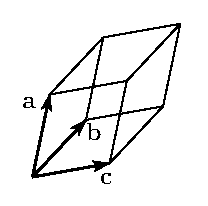
\includegraphics{piped}
      \end{center}
      \end{efig}
        }%
determine a parallelepiped 
(three dimensional parallelogram). Its volume is given by the formula
\begin{impeqn}\label{eq piped volume}
\begin{align*}
\text{volume of parallelepiped with edges $\va,\ \vb,\ \vc\ 
=\ \left|
\det\left[\begin{matrix}a_1&a_2&a_3\\ b_1&b_2&b_3\\ c_1&c_2&c_3\end{matrix}\right]
\right|$}
\end{align*}
\end{impeqn}
The determinant of a $3\times 3$ matrix can be defined in terms
of some $2\times 2$ determinants by
%      \begin{wfig} 
      \begin{center}
      \includegraphics{det2}%\qquad\null
      \end{center}
%      \end{wfig}
This formula is called ``expansion along the top row''. There
is one term in the formula for each entry in the top row of the $3\times 3$
matrix. The term is
a sign times the entry itself times the determinant of the $2\times 2$ matrix
gotten by deleting the row and column that contains the entry. The sign
alternates, starting with a $+$. 

We shall not prove this formula completely here\footnote{For a full derivation, see Example \ref{eg:GEOcross}}. It gets a little tedious.
But, there is one case in which we can easily verify that the volume of the 
parallelepiped is really given by the absolute value of the
claimed determinant. If the vectors $\vb$ and $\vc$ happen to lie
in the $xy$ plane, so that $b_3=c_3=0$, then 
\begin{align*}
\det\left[\begin{matrix}a_1&a_2&a_3\\ b_1&b_2&0\\ c_1&c_2&0\end{matrix}\right]
&=a_1(b_20-0c_2) -a_2(b_10-0c_1) +a_3(b_1c_2-b_2c_1)\\
&=a_3(b_1c_2-b_2c_1)
\end{align*}
The first factor, $a_3$, is the $z$-coordinate of the one vector not contained in the $xy$-plane. It 
is (up to a sign) the height of the parallelepiped. The second factor is,
up to a sign, the area of the parallelogram determined by $\vb$
and $\vc$. This parallelogram forms the base of the parallelepiped. 
The product is indeed, up to a sign, the volume of the parallelepiped.
That the formula is true in general is a consequence of the fact (that
we will not prove) that the value of a determinant does not change when
one rotates the coordinate system and that one can always rotate
our coordinate axes around so that $\vb$ and $\vc$ both lie in the
$xy$-plane. 


%%%%%%%%%%%%%%%%%%%%%%%%%%%%%%%%%%%%%%%%%%%%%%%%%%%%%%%
\subsection{The Cross Product}
%%%%%%%%%%%%%%%%%%%%%%%%%%%%%%%%%%%%%%%%%%%%%%%%%%%%%%%
We have already seen two different products involving vectors ---
the multiplication of a vector by a scalar 
and the dot product of two vectors. The dot product of two vectors
yields a scalar. We now introduce another product 
of two vectors, called the \emph{cross product}. The cross product of
two vectors will give a vector. There are applications which have two 
vectors as inputs and produce one vector as an output, and which are related
to the cross product. Here is a very brief mention of two such applications. 
We will look at them in much more detail later. 
\begin{itemize}
\item 
Consider a parallelogram in three dimensions.
A parallelogram is naturally determined by the two vectors that define 
its sides.
One measure of the size of a parallelogram is its area. 
One way to specify the orientation of the parallelogram is to give a vector
that is perpendicular to it. 
A very compact way to encode both the area and the orientation of
the parallelogram is to give a vector whose direction is perpendicular 
to the plane in which it lies and whose magnitude is its area.
We shall see that such a vector can be easily constructed by taking the cross product (definition coming shortly) of the two vectors that give
the sides of the parallelogram.

      \begin{nfig} 
      \begin{center}
      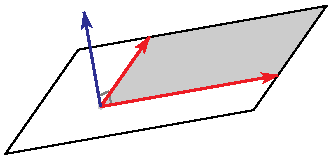
\includegraphics{pgramCross.pdf}
      \end{center}
      \end{nfig}

\item 
Imagine a rigid body which is rotating at a rate $\Omega$ radians per 
second about an axis whose direction is given by the unit vector $\hat\va$. 
Let $P$ be any point on the body. We shall see, in the (optional)
\S\ref{sec rot motion}, that the velocity, $\vv$, of the point $P$ 
is the cross product 
(again, definition coming shortly) of the vector $\Om\hat\va$ with the vector
$\vr$ from any point on the axis of rotation to $P$.
      \begin{nfig} 
      \begin{center}
      \includegraphics{rigidBB}
      \end{center}
      \end{nfig}
\end{itemize}

\noindent
Finally, here is the definition of the cross product. Note that it applies only to vectors in three dimensions.

\begin{defn}[Cross Product]\label{def:crossProd}
The cross product of the vectors $\va=\llt a_1,a_2,a_3\rgt$ and 
$\vb=\llt b_1,b_2,b_3\rgt$ is denoted $\va\times\vb$ 
and is defined by
\begin{align*}
\va\times\vb = \llt a_2b_3-a_3b_2\,,\, a_3b_1-a_1b_3\,,\, a_1b_2-a_2b_1\rgt 
\end{align*}
\end{defn}

Note that each component has the form $a_ib_j-a_jb_i$. The index $i$ of
the first $a$ in component number $k$ of $\va\times\vb$
is just after $k$ in the list $1,2,3,1,2,3,1,2,3,\cdots$. 
The index $j$ of the first $b$ is just before $k$ in the list. 
\begin{align*}
(\va\times\vb)_k
=a_{{\rm just\  after\  }k}\ b_{{\rm just\  before\  }k}
-a_{{\rm just\  before\  }k}\ b_{{\rm just\  after\  }k}
\end{align*}
For example, for component number $k=3$,
\begin{align*}
\left.{\text{``just after 3'' is 1}}\atop{\text{``just before 3'' is 2}}\right\}
\implies (\va\times\vb)_3= a_1b_2-a_2b_1
\end{align*}


There is a much better way to remember this definition. Recall that
a $2\times 2$ matrix is an array of numbers having two rows and two columns
and that the determinant of a $2\times 2$ matrix is  defined by
\begin{align*}
\det \left[\begin{matrix}a& b\\ c&d\end{matrix}\right]=ad-bc
\end{align*}
It is the product of the entries on the diagonal minus the product
of the entries not on the diagonal. 

A $3\times 3$ matrix is an array of
numbers having three rows and three columns.
\begin{align*}
 \left[\begin{matrix}i& j &k\\ a_1&a_2&a_3\\ b_1&b_2&b_3\end{matrix}\right]
\end{align*}
You will shortly see why the entries in the top row have been given the
rather peculiar names $i$, $j$ and $k$. The determinant of a $3\times 3$ 
matrix can be defined in terms of some $2\times 2$ determinants by
      \begin{center}
      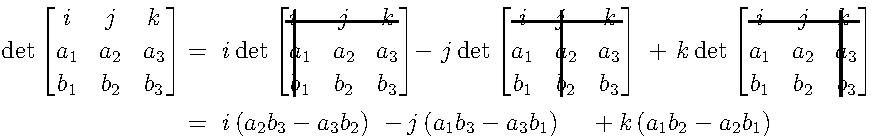
\includegraphics{det.pdf}
      \end{center}
This formula is called ``expansion of the determinant along the top row''. 
There is one term in the formula for each entry in the top row. The term is
a sign times the entry itself times the determinant of the $2\times 2$ matrix
gotten by deleting the row and column that contains the entry. The sign
alternates, starting with a $+$. If we now replace $i$ by $\hi$, $j$ by $\hj$ 
and $k$ by $\hk$, we get exactly the formula for $\va\times \vb$
of Definition \ref{def:crossProd}. That is the reason for the peculiar 
choice of names for the matrix entries. So
\begin{align*}
\va\times\vb
&=\det\left[\begin{matrix}\hi& \hj &\hk\\ 
                            a_1&a_2&a_3\\ 
                            b_1&b_2&b_3\end{matrix}\right] \\
&=\hi\big(a_2b_3-a_3b_2) -\hj(a_1b_3-a_3b_1) +\hk(a_1b_2-a_2b_1)
\end{align*}
is a mnemonic device for remembering the definition of $\va\times\vb$.
It is also good from the point of view of evaluating $\va\times\vb$.
Here are several examples in which we use the determinant mnemonic device to 
evaluate cross products.

\begin{eg}\label{eg:GEOcrossijji}
In this example, we'll use the mnemonic device to compute two very simple cross
products. First
      \begin{center}
      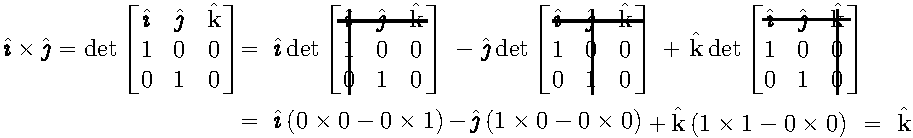
\includegraphics{detij.pdf}
      \end{center}
Second
      \begin{center}
      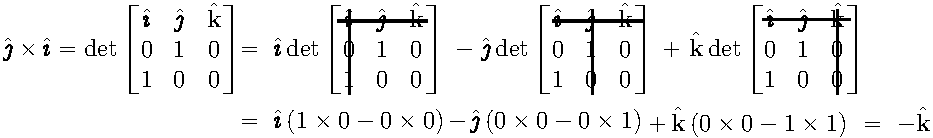
\includegraphics{detji.pdf}
      \end{center}
Note that, unlike most (or maybe even all) products that you have seen before, $\hi\times\hj$ is \emph{not} the same as $\hj\times\hi$!
\end{eg}

\begin{eg}\label{eg:GEOcrossEgA}
In this example, we'll use the mnemonic device to compute two more complicated cross products. Let $\va=\llt 1,2,3 \rgt$ and $\vb=\llt 1,-1,2 \rgt$. First
      \begin{center}
      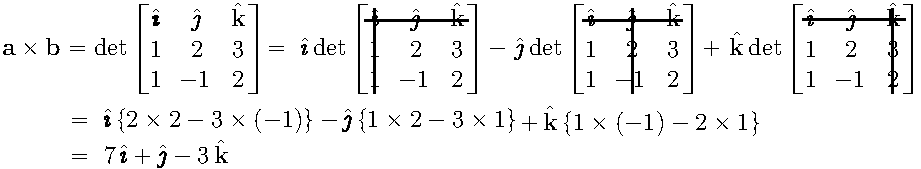
\includegraphics{detEgA1.pdf}
      \end{center}
Second
      \begin{center}
      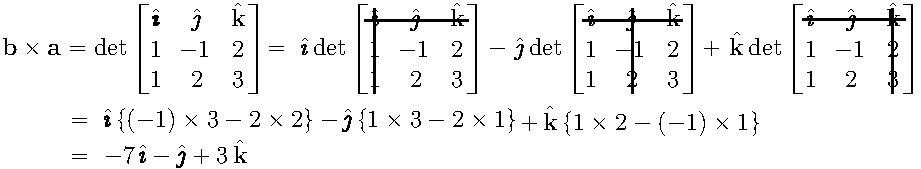
\includegraphics{detEgA2.pdf}
      \end{center}
Here are some important observations.
\begin{itemize}
\item 
The vectors $\va\times\vb$ and $\vb\times\va$ are not the same! In fact
    $\vb\times\va=-\va\times\vb$. We shall see in Theorem \ref{thm:crossPppties}
    below that this was not a fluke.

\item
The vector $\va\times\vb$ has dot product zero with both $\va$ and $\vb$.
So the vector  $\va\times\vb$ is prependicular to both $\va$ and $\vb$. 
We shall see in Theorem \ref{thm:crossPppties} below that this was also not a fluke.
\end{itemize}
\end{eg}

\begin{eg}\label{eg:GEOcrossEgB}
Yet again we use the mnemonic device to compute a more complicated cross product. This time let $\va=\llt 3,2,1 \rgt$ and $\vb=\llt 6,4,2 \rgt$. Then
      \begin{center}
      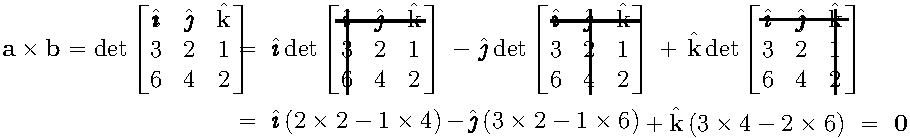
\includegraphics{detEgB.pdf}
      \end{center}
We shall see in Theorem \ref{thm:crossPppties}
    below that it is not a fluke that the cross product is $\vZero$.
It is a consequence of the fact that $\va$ and $\vb=2\va$ are parallel. 
\end{eg}

We now move on to learning about the properties of the cross product.
Our first properties
lead up to a more intuitive geometric definition of $\va\times\vb$, which is better for interpreting $\va\times\vb$. 
 These properties of the cross product, which state that  $\va\times\vb$
is a vector and then determine its direction and length, are as follows.
We will collect these properties, and a few others, into a theorem shortly.
\begin{enumerate}[(1)]
\setcounter{enumi}{-1}
\item $\va,\vb\text{ are vectors in three dimensions and }
\va\times\vb\text{ is a vector in three dimensions}$.

\item $\va\times\vb$ is perpendicular to both  $\va$ and $\vb$.

\textit{Proof}: To check that $\va$ and $\va\times \vb$ are perpendicular, 
one just has to check that the dot product $\va\cdot(\va\times \vb)=0$.
The six terms in 
\begin{equation*}
\va\cdot(\va\times \vb)=
a_1(a_2b_3-a_3b_2)+a_2(a_3b_1-a_1b_3)+a_3(a_1b_2-a_2b_1)
\end{equation*} 
cancel pairwise. The computation showing that $\vb\cdot(\va\times \vb)=0$ 
is similar.

\bigskip
\item $|\va\times\vb|=|\va|\,|\vb|\sin\theta
\text{ where $0\le\theta\le\pi$ is the angle between $\va$ and $\vb$}$

$\phantom{|\va\times\vb|}=\text{the area of the parallelogram
with sides $\va$ and $\vb$}\qquad\qquad\quad
\smash{\raisebox{-0.2\height}{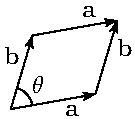
\includegraphics{area.pdf}}}$

\textit{Proof}: 
%This follows from 
%$|\va\times\vb|^2
%=|\va|^2|\vb|^2-(\va\cdot\vb)^2
%=|\va|^2|\vb|^2(1-\cos^2\theta)$ which in turn is gotten by comparing
The formula $|\va\times\vb|=|\va|\,|\vb|\sin\theta$ is gotten by verifying that
\begin{align*}
|\va\times\vb|^2
&=\big(\va\times\vb\big)\cdot\big(\va\times\vb\big) \\
&=(a_2b_3-a_3b_2)^2+(a_3b_1-a_1b_3)^2+ (a_1b_2-a_2b_1)^2\\
&=a_2^2b_3^2-2a_2b_3a_3b_2+a_3^2b_2^2
+a_3^2b_1^2-2a_3b_1a_1b_3+a_1^2b_3^2\\&\hskip0.5in
+a_1^2b_2^2-2a_1b_2a_2b_1+a_2^2b_1^2\\
\intertext{is equal to}
|\va|^2\,|\vb|^2\sin^2\theta
&=|\va|^2|\vb|^2(1-\cos^2\theta)\\
&=|\va|^2|\vb|^2-(\va\cdot\vb)^2 \\
&=\big(a_1^2+a_2^2+a_3^2\big)\big(b_1^2+b_2^2+b_3^2\big)
-\big(a_1b_1+a_2b_2+a_3b_3\big)^2\\
&=a_1^2b_2^2+a_1^2b_3^2+a_2^2b_1^2+a_2^2b_3^2+a_3^2b_1^2+a_3^2b_2^2\\
&\hskip0.5in
 -\big(2a_1b_1a_2b_2+2a_1b_1a_3b_3+2a_2b_2a_3b_3\big)\\
\end{align*}
To see that $|\va|\,|\vb|\sin\theta$ is the area of the parallelogram
with sides $\va$ and $\vb$, just recall that the area of any parallelogram
is given by the length of its base times its height. Think of $\va$ as the
base of the parallelogram. Then $|\va|$ is the length of the base
and $|\vb|\sin\theta$ is the height.
      \begin{efig} 
      \begin{center}
      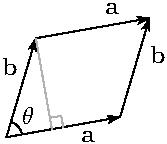
\includegraphics{areaB.pdf}
      \end{center}
      \end{efig}


\end{enumerate}

\noindent
These properties almost determine $\va\times\vb$. Property 1 forces
the vector $\va\times\vb$ to lie on the line perpendicular to the
plane containing $\va$ and $\vb$. There are precisely two vectors
on this line that have the length given by property 2. In the left hand
figure of
      \begin{efig} 
      \begin{center}
      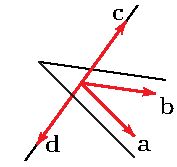
\includegraphics{crossLL.pdf}\qquad\quad
      \raisebox{-0.05\height}{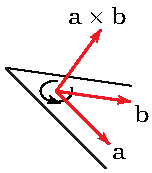
\includegraphics{crossRR.pdf}}\qquad\quad
%    \raisebox{0.05\height}{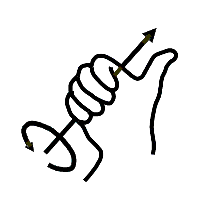
\includegraphics[scale=0.8]{Right-hand_rule.pdf}}
    \raisebox{0.2\height}{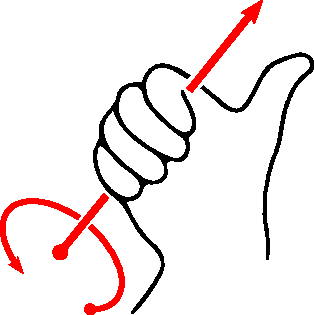
\includegraphics[scale=0.4]{RHR.pdf}}
      \end{center}
      \end{efig}
the two vectors are labeled $\vc$ and $\vd$. Which of these two
candidates is correct is determined by the right hand rule\footnote{That 
the cross product uses the right hand rule, rather than the left hand rule, is an example of the tyranny of the masses --- only roughly 10\% 
of humans are left-handed. }, which says
that if you form your right hand into a fist with your fingers curling from 
$\va$ to $\vb$, then when you stick your thumb straight out from
the fist, it points in the direction of $\va\times\vb$. This is
illustrated in the figure on the right 
above
\footnote{This figure is a variant of 
https:/\hskip-1pt/commons.wikimedia.org/wiki/File:Right\_hand\_rule\_simple.png
}.
The important special cases

\begin{enumerate}[(1)]
\setcounter{enumi}{2}
\item $\hi\times\hj=\phantom{-}\hk,\ \ \ \hj\times\hk=\phantom{-}\hi,\ \ \  \hk\times\hi=\phantom{-}\hj$ \\
      $\hj\times\hi=-\hk,\ \ \ \hk\times\hj=-\hi,\ \ \ \hi\times\hk=-\hj$

all follow directly from the definition of the cross product (see, for example,
Example \ref{eg:GEOcrossijji}) and all 
obey the right hand rule.  Combining properties 1, 2 and the right hand 
rule give the geometric definition of $\va\times\vb$. To remember
these three special cases, just remember this figure.
      \begin{efig} 
      \begin{center}
      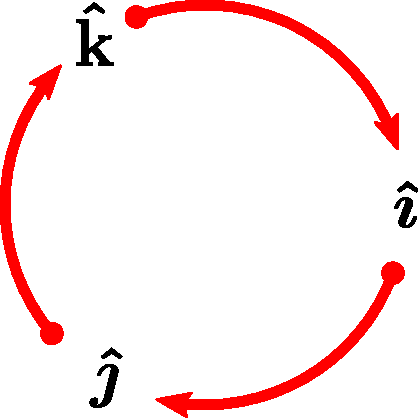
\includegraphics[scale=0.3]{cp_circle.pdf}
      \end{center}
      \end{efig}
The product of any two standard basis vectors, taken in the order of 
the arrows in the figure, is the third standard basis vector.
Going against the arrows introduces a minus sign.


\item $\va\times\vb=|\va|\,|\vb|\sin\theta\ \hn
\text{ where $\theta$ is the angle between $\va$ and $\vb$, }
|\hn|=1,\ \hn\perp\va,\vb$
  and $(\va,\vb,\hn)$ obey the right hand rule.

\textit{Outline of Proof}: We have already seen that the right hand side
has the correct length and, except possibly for a sign, direction.
To check that the right hand rule holds in
general, rotate your coordinate system around\footnote{Note that as you 
translate or rotate the coordinate system, the right hand rule is preserved. 
If $(\va,\vb,\hn)$ obey the right hand rule so do their rotated and 
translated versions.} 
so that $\va$ points along
the positive $x$ axis and $\vb$ lies in the $xy$-plane with positive
$y$ component. That is $\va=\alpha\hi$ and $\vb=\beta\hi+\gamma
\hj$ with $\alpha,\gamma\ge 0$. Then 
$\va\times\vb=\alpha\hi\times(\beta\hi+\gamma\hj)
=\alpha\beta\,\hi\times\hi+\alpha\gamma\,\hi\times\hj$. The
first term vanishes by property 2, because the angle $\theta$ between $\hi$
and $\hi$ is zero. So, by property 3, 
$\va\times\vb= \alpha\gamma\hk$ points
along the positive $z$ axis, which is consistent with the right hand rule.

\end{enumerate}

\noindent  The analog of property 7 of the dot product (which says that
$\va\cdot\vb$ is zero if and only if  $\va=\vZero$ or $\vb=\vZero$ or  $\va\perp\vb$) follows
immediately from property 2.

\begin{enumerate}[(1)]
\setcounter{enumi}{4}

\item $\va\times\vb=\vZero\iff \va=\vZero \text{ or }\vb=\vZero 
\text{ or }\va\parallel\vb$

\end{enumerate}

\noindent
The remaining properties are all tools for
helping do computations with cross products.
Here is a theorem which summarizes the properties of the cross product.
We have already seen the first five. The other properties are all tools 
for helping do computations with cross products.

\begin{theorem}[Properties of the Cross Product]\label{thm:crossPppties}
\begin{enumerate}[(1)]
\setcounter{enumi}{-1}

\item $\va,\vb\text{ are vectors in three dimensions and }
\va\times\vb\text{ is a vector in three dimensions}$.

\item $\va\times\vb$ is perpendicular to both  $\va$ and $\vb$.

\bigskip
\item $|\va\times\vb|=|\va|\,|\vb|\sin\theta
\text{ where $\theta$ is the angle between $\va$ and $\vb$}$

$\phantom{|\va\times\vb|}=\text{the area of the parallelogram
with sides $\va$ and $\vb$}\qquad
\smash{\raisebox{-0.1\height}{\includegraphics{area.pdf}}}$

\item $\hi\times\hj=\hk,\ \hj\times\hk=\hi,\ \hk\times\hi=\hj$


\item $\va\times\vb=|\va|\,|\vb|\sin\theta\ \vn
\text{ where $\theta$ is the angle between $\va$ and $\vb$, }
|\vn|=1,\\ \vn\perp\va,\vb$
  and $(\va,\vb,\vn)$ obey the right hand rule.

\item $\va\times\vb=\vZero\iff \va=\vZero \text{ or }\vb=\vZero 
\text{ or }\va\parallel\vb$

%
%\end{enumerate}
%\end{theorem}
%
%\addtocounter{theorem}{-1}
%\begin{theorem}[continued]
%\begin{enumerate}[(1)]
%\setcounter{enumi}{5}

\item $\va\times \vb=-\vb\times\va$

\item $(s\va)\times \vb=\va\times(s\vb)=s(\va\times \vb)$ for any scalar
(i.e. number) $s$.

\item $\va\times(\vb+\vc)=\va\times\vb+\va\times \vc$

\item $\va\cdot(\vb\times\vc)=(\va\times\vb)\cdot\vc$

\item $\va\times(\vb\times\vc)=(\vc\cdot\va)\vb -(\vb\cdot\va)\vc$
\end{enumerate}

\end{theorem}
\begin{proof}
We have already seen the proofs up to number 5. Numbers 6, 7 and 8 
follow immediately from the definition, using a little algebra. To prove 
numbers 9 and 10 we just write out the definitions of the left hand sides 
and the right hand sides and observe that they are equal.

\medskip
\noindent (9)\ \ \ The left hand side is
\begin{align*}
\va\cdot(\vb\times\vc)
&=\llt a_1,a_2,a_3\rgt\cdot
      \llt b_2c_3-b_3c_2\,,\, b_3c_1-b_1c_3\,,\, b_1c_2-b_2c_1\rgt\\
&=\textcolor{blue}{a_1b_2c_3} - \textcolor{blue}{a_1b_3c_2} 
    + \textcolor{orange}{a_2b_3c_1} - \textcolor{orange}{a_2b_1c_3} 
    + a_3b_1c_2 - a_3b_2c_1
\end{align*}
The right hand side is
\begin{align*}
(\va\times\vb)\cdot\vc
&=\llt a_2b_3-a_3b_2\,,\, a_3b_1-a_1b_3\,,\, a_1b_2-a_2b_1\rgt\cdot
       \llt c_1,c_2,c_3\rgt \\
&=\textcolor{orange}{a_2b_3c_1} - a_3b_2c_1 + a_3b_1c_2 
- \textcolor{blue}{a_1b_3c_2} + \textcolor{blue}{a_1b_2c_3} 
- \textcolor{orange}{a_2b_1c_3}
\end{align*}
The left and right hand sides are the same.

\medskip
\noindent (10)\ \ \ We will give the straightforward, but slightly tedious,
computations in (the optional) \S\ref{sec vector identities}.
 \end{proof}


\begin{warning}\label{warning:GEOMcross} 
Take particular care with properties 6 and 10. They are 
counterintuitive and are a frequent source of errors. In particular, 
for general vectors $\va$, $\vb$, $\vc$, the cross product is neither
commutative nor associative, meaning that
\begin{align*}
\va\times\vb&\ne\vb\times\va\\
\va\times(\vb\times\vc)&\ne (\va\times\vb)\times\vc
\end{align*} 
For example
\begin{align*}
\hi\times(\hi\times\hj)
&=\hi\times\hk=-\hk\times\hi =-\hj\\
(\hi\times \hi)\times\hj&= \vZero \times\hj=\vZero\\
\end{align*} 
\end{warning}

\begin{eg}\label{eg:GEOcross}
As an illustration of the properties of the dot and cross product, we now
derive the formula for the volume of the parallelepiped with edges 
$\va=\llt a_1,a_2,a_3\rgt $, $\vb = \llt b_1,b_2,b_3\rgt $, 
$\vc = \llt c_1,c_2,c_3\rgt $ that was mentioned in 
\S\ref{sec:GEOparallelogram}.
\vadjust{
      \begin{efig} 
      \begin{center}
      \includegraphics{pipedVolume.pdf}
      \end{center}
      \end{efig}
        }%
The volume of the parallelepiped is the area of its base times its 
height\footnote{This is a simple integral calculus exercise.}.
The base is the parallelogram with sides $\vb$ and
$\vc$. Its area is the length of its base, which is $|\vb|$,
times its height, which is $|\vc|\,\sin\theta$. (Drop a 
perpendicular from the head of $\vc$ to the line containing $\vb$). 
Here $\theta$ is the angle between $\vb$ and $\vc$. So the area of the 
base is $|\vb|\,|\vc|\,\sin\theta= |\vb\times\vc|$, by 
property 2 of the cross product. To get the height of the parallelepiped, 
we drop a perpendicular from the head of $\va$ to the line that passes 
through the tail of $\va$ and is perpendicular to the base of the parallelepiped. In other words, from
the head of $\va$ to the line that contains both the head and the tail
of $\vb\times\vc$. So the height of the parallelepiped is
$|\va|\,|\cos\varphi|$.  (The absolute values have been included because 
if the angle between $\vb\times\vc$ and $\va$ happens to be greater
than $90^\circ$, the $\cos\varphi$ produced by taking the dot product of 
$\va$ and  $(\vb\times\vc$) will be negative.) All together
\begin{align*}
\text{volume of parallelepiped}
&=(\text{area of base})\,(\text{height})\\
&=|\vb\times\vc|\ |\va|\ |\cos\varphi|\\
&=\big|\va\cdot(\vb\times\vc)\big|\\
&=\left|a_1 (\vb\times\vc)_1 +a_2 (\vb\times\vc)_2 
               +a_3 (\vb\times\vc)_3\right|\\
&=\left|a_1\det\left[\begin{matrix}b_2&b_3\\ c_2&c_3\end{matrix}\right] 
        -a_2 \det\left[\begin{matrix}b_1&b_3\\ c_1&c_3\end{matrix}\right] 
               +a_3\det\left[\begin{matrix}b_1&b_2\\ c_1&c_2\end{matrix}\right]\right|\\
&=\left|\det\left[\begin{matrix}a_1&a_2&a_3\\
                          b_1&b_2&b_3\\
                          c_1&c_2&c_3\end{matrix}\right]\right|
\end{align*}

\end{eg}


\begin{eg}\label{eg:GEOcrossConcrete}
As a concrete example of the computation of the volume of a parallelepiped,
we consider the parallelepiped with edges
\begin{align*}
\va &= \llt 0,1,2\rgt \\
\vb &= \llt 1,1,0\rgt \\
\vc &= \llt 0,1,0\rgt
\end{align*}
Here is a sketch.
\vadjust{
      \begin{efig} 
      \begin{center}
      \includegraphics{pipedVolumeEg.pdf}
      \end{center}
      \end{efig}
        }%
The base of the parallelepiped is the parallelogram with sides $\vb$ and $\vc$.
It is the shaded parallelogram in the sketch above. As
\begin{align*}
\vb\times\vc
&=\det\left[\begin{matrix}\hi& \hj &\hk\\ 
                            1&1&0\\ 
                            0&1&0\end{matrix}\right] \\
&=\hi\det\left[\begin{matrix} 1&0\\ 
                              1&0\end{matrix}\right]
  -\hj\det\left[\begin{matrix}1&0\\ 
                              0&0\end{matrix}\right] 
   +\hk\det\left[\begin{matrix} 1&1\\ 
                                0&1\end{matrix}\right] \\
&=\hi\big(1\times 0-0\times 1) -\hj(1\times 0-0\times 0) 
                  +\hk(1\times 1-1\times 0) \\
&=\hk
\end{align*}
We should not be surprised that $\vb\times\vc$ has direction $\hk$.
\begin{itemize}\itemsep1pt \parskip0pt \parsep0pt
\item[$\circ$]
$\vb\times\vc$ has to be perpendicular to both $\vb$ and $\vc$ and 
\item[$\circ$]
both $\vb$ and $\vc$ lie in the $xy$-plane, 
\item[$\circ$]
so that $\vb\times\vc$ has to the perpendicular to the $xy$-plane,
\item[$\circ$]
so that $\vb\times\vc$ has to the parallel to the $z$-axis.
\end{itemize}
The area of the base, i.e. of the shaded parallelogram in the figure above,
is
\begin{equation*}
|\vb\times\vc| = |\hk| =1
\end{equation*}
and the volume of the parallelepiped is
\begin{equation*}
|\va\cdot (\vb\times\vc)|
= |\llt 0,1,2\rgt\cdot\llt 0,0,1\rgt|=2
\end{equation*}

\end{eg}

%%%%%%%%%%%%%%%%%%%%%%%%%%%%%%%%%%%%%%%%%%%%%%%%%%%%%%%%%%%%%%%%%%%
\subsection{(Optional) Some Vector Identities}
\label{sec vector identities}

Here are a few identities involving dot and cross products.
\begin{lemma}\label{lem:tripProd}
\begin{enumerate}[(a)]
\item\ \ \ 
$\va\cdot(\vb\times\vc)=(\va\times\vb)\cdot\vc$
\item\ \ \ 
$\va\times(\vb\times\vc)=(\vc\cdot\va)\vb-(\vb\cdot\va)\vc$
\item\ \ \ 
           $\va\times(\vb\times\vc) + 
            \vb\times(\vc\times\va) +
            \vc\times(\va\times\vb) =\vZero$
\end{enumerate}
\end{lemma}
\begin{proof} (a)
We proved this in Theorem \ref{thm:crossPppties}, by evaluating the left and right hand  sides, and observing that they are the same.
Here is a second proof, in which we again write out both sides, 
but this time we express them in terms of determinants.
\begin{align*}
\va\cdot\vb\times\vc
&=(a_1,a_2,a_3)\cdot\det\left[\begin{matrix}\hi&\hj&\hk\\
                                       b_1&b_2&b_3\\
                                       c_1&c_2&c_3\end{matrix}\right]\\
&=a_1\det\left[\begin{matrix}
                                       b_2&b_3\\
                                       c_2&c_3\end{matrix}\right]
                             -a_2\det\left[\begin{matrix}
                                       b_1&b_3\\
                                       c_1&c_3\end{matrix}\right]
                             +a_3\det\left[\begin{matrix}
                                       b_1&b_2\\
                                       c_1&c_2\end{matrix}\right]\\
&=\det\left[\begin{matrix}a_1&a_2&a_3\\
                                       b_1&b_2&b_3\\
                                       c_1&c_2&c_3\end{matrix}\right]\\[0.1in]
\va\times\vb\cdot\vc
&=\det\left[\begin{matrix}\hi&\hj&\hk\\
                     a_1&a_2&a_3\\
                     b_1&b_2&b_3\end{matrix}\right]\cdot(c_1,c_2,c_3)\\
&=c_1\det\left[\begin{matrix}
                                       a_2&a_3\\
                                       b_2&b_3\end{matrix}\right]
                             -c_2\det\left[\begin{matrix}
                                       a_1&a_3\\
                                       b_1&b_3\end{matrix}\right]
                             +c_3\det\left[\begin{matrix}
                                       a_1&a_2\\
                                       b_1&b_2\end{matrix}\right]\\
&=\det\left[\begin{matrix}c_1&c_2&c_3\cr a_1&a_2&a_3\\
                                       b_1&b_2&b_3\\
                                       \end{matrix}\right]
\end{align*}
Exchanging two rows in a determinant changes the sign of the determinant.
Moving the top row of a $3\times 3$ determinant to the bottom row requires
two exchanges of rows.
So the two $3\times 3$ determinants are equal.

\noindent (b)
The proof is not exceptionally difficult --- just write out both sides and grind.
Substituting in
\begin{equation*}
\vb\times\vc
\ =\ (b_2c_3-b_3c_2)\hi-(b_1c_3-b_3c_1)\hj + (b_1c_2-b_2c_1)\hk
\end{equation*}
gives, for the left hand side,
\begin{align*}
\va\times(\vb\times\vc)
=\phantom{-}&\!\!\!\det\left[\begin{matrix}\hi&\hj &\hk\\
                     a_1&a_2&a_3\\
                     b_2c_3-b_3c_2&-b_1c_3+b_3c_1&b_1c_2-b_2c_1
                     \end{matrix}\right]\\[0.1in]
=\phantom{-}&\hi\big[a_2(b_1c_2-b_2c_1)-a_3(-b_1c_3+b_3c_1)\big]\\
-&\hj\big[a_1(b_1c_2-b_2c_1)-a_3(b_2c_3-b_3c_2)\big]\\
+&\hk\big[a_1(-b_1c_3+b_3c_1)-a_2(b_2c_3-b_3c_2)\big]
\end{align*}
On the other hand, the right hand side
\begin{align*}
(\va\cdot\vc)\vb-(\va\cdot\vb)\vc
&=(a_1c_1+a_2c_2+a_3c_3)(b_1\hi+b_2\hj+b_3\hk) \\
     &\hskip1in -(a_1b_1+a_2b_2+a_3b_3)(c_1\hi+c_2\hj+c_3\hk)
\\
&=\phantom{-}
\hi\ \big[\textcolor{blue}{a_1b_1c_1}
         +a_2b_1c_2+a_3b_1c_3-
         \textcolor{blue}{a_1b_1c_1}
         -a_2b_2c_1-a_3b_3c_1\big]
\\
&\phantom{=}+\hj\ \big[a_1b_2c_1
      +\textcolor{blue}{a_2b_2c_2}
      +a_3b_2c_3-a_1b_1c_2
      -\textcolor{blue}{a_2b_2c_2}
      -a_3b_3c_2\big]
\\
&\phantom{=}+\hk\ \big[a_1b_3c_1+a_2b_3c_2
          +\textcolor{blue}{a_3b_3c_3}
          -a_1b_1c_3-a_2b_2c_3
          -\textcolor{blue}{a_3b_3c_3}\big]
\\
&=\phantom{-}
\hi\ [a_2b_1c_2+a_3b_1c_3-a_2b_2c_1-a_3b_3c_1]
\\
&\phantom{=}+\hj\ [a_1b_2c_1+a_3b_2c_3-a_1b_1c_2-a_3b_3c_2]
\\
&\phantom{=}+\hk\ [a_1b_3c_1+a_2b_3c_2-a_1b_1c_3-a_2b_2c_3]
\end{align*}
The last formula that we had for the left hand side is the same as the last formula we had for the right hand side. Oof! This is a little tedious
to do by hand. But any computer algebra system will do it for you in a 
flash.


\noindent (c)
We just apply part (b) three times
\begin{align*}
          &\va\times(\vb\times\vc) + 
            \vb\times(\vc\times\va) +
            \vc\times(\va\times\vb)  \\
&\hskip0.5in= (\vc\cdot\va)\vb-(\vb\cdot\va)\vc
            + (\va\cdot\vb)\vc-(\vc\cdot\vb)\va
            + (\vb\cdot\vc)\va-(\va\cdot\vc)\vb \\
&\hskip0.5in=\vZero            
\end{align*}
\end{proof}



%%%%%%%%%%%%%%%%%%%%%%%%%%%%%%%%%%%%%%%%%%%%%%%%%%%%%%%%%%%%%%%%%%%
\subsection{(Optional) Application of Cross Products to Rotational Motion}
\label{sec rot motion}
%%%%%%%%%%%%%%%%%%%%%%%%%%%%%%%%%%%%%%%%%%%%%%%%%%%%%%%%%%%%%%%%%%%
In most computations involving rotational motion, the cross product shows
up in one form or another. This is one of the main applications of the cross
product. Consider, for example, a rigid body which is rotating 
 at a constant rate of $\Omega$ radians per second about an axis 
whose direction is given by the unit vector $\hat\va$. Let $P$ be any point
on the body. Let's figure out its velocity. Pick any point on the axis
of rotation and designate it as the origin of our coordinate system. Denote
by $\vr$ the vector from the origin to the point $P$. Let $\theta$ denote
the angle between $\hat\va$ and $\vr$. As time progresses the point $P$
sweeps out a circle of radius $R=|\vr\,|\sin\theta$.
      \begin{efig} 
      \begin{center}
      \includegraphics{rigid}
      \end{center}
      \end{efig}
In one second $P$ travels along an arc that subtends an angle of 
$\Omega$ radians, which is the fraction $\tfrac{\Omega}{2\pi}$ 
of a full circle.  The length of this arc is
$\tfrac{\Omega}{2\pi}\times 2\pi R=\Omega R=\Omega|\vr\,|\sin\theta$ so $P$ travels the distance $\Omega|\vr\,|\sin\theta$
in one second and its speed, which is also the length of its velocity vector,
is $\Omega|\vr\,|\sin\theta$. 

Now we just need to figure out the direction
of the velocity vector. That is, the direction of motion of the point $P$.
Imagine that both $\hat\va$ and $\vr$ lie in the plane of a piece of paper, 
as in the figure above. Then $\vv$ points either straight into 
or straight out of the page and consequently is perpendicular
to both $\hat\va$ and $\vr$. To distinguish between the ``into the page''
and ``out of the page'' cases, let's impose the conventions that 
$\Omega>0$ and the axis of rotation $\hat\va$ is chosen to obey the right hand
 rule, meaning that if the thumb of
your right hand is pointing in the direction $\hat\va$, then your fingers
are pointing in the direction of motion of the rigid body.  Under these
conventions, the velocity vector $\vv$ obeys
\begin{itemize}
\item $|\vv|=\Omega|\vr||\hat\va|\sin\theta$
\item $\vv\perp\hat\va,\vr$
\item $(\hat\va,\vr,\vv)$ obey the right hand rule
\end{itemize}
That is, $\vv$ is exactly $\Omega\hat\va\times\vr$. It is conventional
to define the ``angular velocity'' of a rigid body to be vector
$\mathbf{\Omega}=\Omega\hat\va$. That is, the vector with length given 
by the rate of rotation and direction given by the axis of rotation 
of the rigid body. In particular, the bigger the rate of rotation, the longer
the angular velocity vector. In terms of this angular 
velocity vector, the velocity of the point $P$ is
\begin{align*}
\vv=\mathbf{\Omega}\times\vr
\end{align*}

%%%%%%%%%%%%%%%%%%%%%%%%%%%%%%%%%%%%%%%%%%%%%%%%%%%%%%%%%%%%%%%%%%%
\subsection{(Optional) Application of Cross Products to Rotating Reference Frames}\label{sec rot frame}
%%%%%%%%%%%%%%%%%%%%%%%%%%%%%%%%%%%%%%%%%%%%%%%%%%%%%%%%%%%%%%%%%%%

Imagine a moving particle that is being tracked by two observers.
\begin{enumerate}[(a)]
\item One observer is fixed (out in space) and measures the position of 
  the particle to be $\big(X(t), Y(t), Z(t)\big)$.
\item The other observer is tied to a merry-go-round (the Earth) and 
  measures the position of the particle to be $\big(x(t),y(t),z(t)\big)$.
\end{enumerate}
The merry-go-round is sketched in the figure on the left below. It
is rotating about the $Z$-axis at a (constant) rate of $\Omega$ radians per second.
The vector $\vOmega = \Omega \hk$, whose length is the rate of rotation and
whose direction is the axis of rotation, is called the angular velocity.
\vadjust{
      \begin{efig} 
      \begin{center}
      \includegraphics{merry.pdf}\qquad\qquad
      \includegraphics{merryB.pdf}
      \end{center}
      \end{efig}
        }%
The $x$- and $y$-axes of the moving observer are painted in red on
the merry-go-round. The figure on the right above shows a top view of the
merry-go-round. The $x$- and $y$-axes of the moving observer are again
red. The $X$- and $Y$-axes of the fixed observer are blue.  We are
assuming that at time $0$, the $x$-axis of the moving observer and 
the $X$-axis of the fixed observer coincide. As the merry-go-round
is rotating at $\Om$ radians per second, the angle between the $X$-axis
and $x$-axis after $t$ seconds is $\Omega t$.

As an example, suppose that the moving particle is tied to the tip of the
moving observer's unit $x$ vector. Then
\begin{align*}
x(t) & = 1 &  y(t) &= 0 & z(t) &= 0 \\
X(t) & = \cos(\Om t) &  Y(t) &=\sin(\Om t) & Z(t) &= 0 
\end{align*}
or, if we write $\vr(t) = \big(x(t), y(t), z(t)\big)$ and 
$\vR(t) = \big(X(t), Y(t), Z(t)\big)$, then
\begin{align*}
\vr(t) = (1\,,\,0\,,\,0) \qquad
\vR(t)= \big(\cos(\Om t)\,,\,\sin(\Om t)\,,\,0\Big)
\end{align*}

In general, denote by $\hi(t)$ the coordinates of the unit $x$-vector
of the moving observer at time $t$, as measured by the fixed observer.
Similarly $\hj(t)$ for the unit $y$-vector, and $\hk(t)$ for the unit 
$z$-vector. As the merry-go-round is rotating about the $Z$-axis at a rate of $\Omega$ radians per second, the angle between the $X$-axis
and $x$-axis after $t$ seconds is $\Omega t$, and
\medskip
\begin{align*}
\null\hskip1.5in
\hi(t) &= \big(\cos(\Om t)\,,\,\sin(\Om t)\,,\,0\Big) \\
\hj(t) &= \big(-\sin(\Om t)\,,\,\cos(\Om t)\,,\,0\Big)\hskip0.5in
\smash{\raisebox{-0.45\height}{\includegraphics{merryC.pdf}}} \\
\hk(t) &= \big(0\,,\,0\,,\,1\Big) 
\end{align*}
The position of the moving particle, as seen by the fixed observer is
\begin{align*}
\vR(t) &= x(t)\,\hi(t) + y(t)\,\hj(t) +z(t)\,\hk(t)
\end{align*}
Differentiating, the velocity of the moving particle, as measured 
by the fixed observer is
\begin{align*}
\vV(t)=\diff{\vR}{t} &= \phantom{+}\diff{x}{t}\!(t)\ \hi(t) 
                         + \diff{y}{t}\!(t)\ \hj(t) 
                         + \diff{z}{t}\!(t)\ \hk(t) \\
                     &\phantom{=} +x(t)\diff{\hfill}{t} \hi(t)
                                  +y(t)\diff{\hfill}{t} \hj(t)
                                  +z(t)\diff{\hfill}{t} \hk(t)
\end{align*}
We saw, in the last (optional) \S\ref{sec rot motion}, that
\begin{align*}
\diff{\hfill}{t} \hi(t)=\vOmega\times\hi(t)\quad
\diff{\hfill}{t} \hj(t)=\vOmega\times\hj(t)\quad
\diff{\hfill}{t} \hk(t)=\vOmega\times\hk(t)
\end{align*}
(You could also verify that these are correct by putting in
$\vOmega = (0,0,\Om)$ and explicitly computing the cross products.)
So
\begin{align*}
\vV(t)&= \Big(\diff{x}{t}\!(t)\ \hi(t) 
                         + \diff{y}{t}\!(t)\ \hj(t) 
                         + \diff{z}{t}\!(t)\ \hk(t)\Big)
                     +\vOmega\times\Big(x(t)\ \hi(t)
                                  +y(t)\ \hj(t)
                                  +z(t)\ \hk(t)\Big)
\end{align*}
Differentiating a second time, the acceleration of the moving particle
(which is also $\frac{\vF}{m}$, where $\vF$ is the net force being applied
to the particle and $m$ is the mass of the particle) 
as measured  by the fixed observer is
\begin{align*}
\frac{\vF}{m}
=\vA(t)
=&  \Big(\difftwo{x}{t}\!(t)\ \hi(t) 
                         + \difftwo{y}{t}\!(t)\ \hj(t) 
                         + \difftwo{z}{t}\!(t)\ \hk(t)\Big) \\
& +2\vOmega\times\Big(\diff{x}{t}\!(t)\ \hi(t)
                                  +\diff{y}{t}\!(t)\ \hj(t)
                                  +\diff{z}{t}\!(t)\ \hk(t)\Big) \\
&+\vOmega\times\Big(\vOmega\times\big[x(t)\ \hi(t)
                                  +y(t)\ \hj(t)
                                  +z(t)\ \hk(t)\big]\Big)
\end{align*}
Recall that the angular velocity $\vOmega=(0,0,\Omega)$ does 
not depend on time.
The rotating observer sees $\hi(t)$ as $\hi=(1,0,0)$,
sees $\hj(t)$ as $\hj=(0,1,0)$, and sees $\hk(t)$ as $\hk=(0,0,1)$ and so sees
\begin{align*}
\frac{\vF}{m}
&=\va(t) + 2\vOmega\times\vv(t) +\vOmega\times\big[\vOmega\times\vr(t)\big]
\end{align*}
where, as usual,
\begin{alignat*}{3}
\vv(t) &= \diff{\hfill}{t}\vr(t)
       &&= \Big(\diff{x}{t}(t)\,,\,\diff{y}{t}(t)\,,\,\diff{z}{t}(t)\Big) \\
\va(t) &= \difftwo{\hfill}{t}\vr(t)
    &&= \Big(\difftwo{x}{t}(t)\,,\,\difftwo{y}{t}(t)\,,\,\difftwo{z}{t}(t)\Big)
\end{alignat*}
So the acceleration of the particle seen by the moving observer is
\begin{align*}
\va(t) = \frac{\vF}{m} -  2\vOmega\times\vv(t)      
                     - \vOmega\times\big[\vOmega\times\vr(t)\big]
\end{align*}
Here 
\begin{itemize}\itemsep1pt \parskip0pt \parsep0pt
\item 
   $\vF$ is the sum of all external forces acting on the moving particle, 
\item 
   $\vF_{{\rm cor}}=-2 \vOmega\times\vv(t)$ is called the Coriolis force and
\item
   $ - \vOmega\times\big[\vOmega\times\vr(t)\big]$ is called the centrifugal force.
\end{itemize}
As an example, suppose that you are the moving particle and that
you are at the edge of the merry-go-round. Let's say $t=0$ and you are
at $\hi$. Then $\vF$ is the friction that the surface of the merry-go-round 
applies to the soles of your shoes. If you are just standing there, 
$\vv(t)=\vZero$, so that $\vF_{{\rm cor}}=\vZero$, and the friction 
$\vF$ exactly cancels the centrifugal force 
$-\vOmega\times\big[\vOmega\times\vr(t)\big]$ 
so that you remain at $\hi(t)$. Assume that $\Om>0$. Now suppose that 
you start walking around the edge of the merry-go-round. Then, 
at $t=0$, $\vr=\hi$ and
\begin{itemize}\itemsep1pt \parskip0pt \parsep0pt
\item 
   if you walk in the direction of rotation (with speed one), as in the figure on the 
   left below, $\vv=\hj$ and the Coriolis force $\vF_{{\rm cor}}=
   -2\Om\hk\times\hj = 2\Om\,\hi$ tries to push you off of 
   the merry-go-round, while
\item 
   if you walk opposite to the direction of rotation (with speed one), as in the figure 
   on the right below,  $\vv=-\hj$ so that the Coriolis force 
   $\vF_{{\rm cor}}=-2\Om\hk\times(-\hj) = -2\Om\,\hi$ tries to pull you
   into the centre of the merry-go-round.
\end{itemize}
      \begin{efig} 
      \begin{center}
      \includegraphics{merryD.pdf}\qquad\qquad
      \includegraphics{merryE.pdf}
      \end{center}
      \end{efig}
On a rotating ball, such as the Earth, the Coriolis force deflects
wind to the right (counterclockwise) in the northern hemisphere
and to the left (clockwise) is the southern hemisphere. In particular,
hurricanes/cyclones/typhoons rotate counterclockwise in the northern
hemisphere and clockwise in the southern hemisphere. On the other
hand, when it comes to water draining out of, for example, a toilet,
Coriolis force effects are dominated by other factors like asymmetry 
of the toilet. 



%%%%%%%%%%%%%%%%%%%%%%%%%%%%%%%%%%%%%%%%%%%%%%%%%%%%%%%%%%%%
\section{Equations of Lines in 2d}\label{sec lines 2d}
%%%%%%%%%%%%%%%%%%%%%%%%%%%%%%%%%%%%%%%%%%%%%%%%%%%%%%%%%%%%
A line in two dimensions can be specified  by giving one point
$(x_0,y_0)$ on the line and one vector $\vd=\llt d_x,d_y\rgt $ 
whose direction is parallel to the line.
\vadjust{
      \begin{efig} 
      \begin{center}
      \includegraphics{twodLine.pdf}
      \end{center}
      \end{efig}
        }%
If $(x,y)$ is any point on the line then the vector $\llt x-x_0,y-y_0\rgt $, 
whose tail is at $(x_0,y_0)$ and whose head is at $(x,y)$,  must be parallel
to $\vd$ and hence must be a scalar multiple of $\vd$. So
\begin{impeqn}[Parametric Equations]\label{eqn par line}
\begin{align*}
   \llt x-x_0,y-y_0\rgt =t \vd
\end{align*}
or, writing out in components,
\begin{align*}
   x-x_0&=t d_x\\
   y-y_0&=t d_y
\end{align*}
\end{impeqn}\noindent
These are called the parametric equations of the line, because they contain
a free parameter, namely $t$. As $t$ varies from $-\infty$ to $\infty$,
the point $(x_0+td_x,y_0+td_y)$ traverses the entire line.

It is easy to eliminate the parameter $t$ from the equations. Just 
multiply $x-x_0=t d_x$ by $d_y$, multiply $y-y_0=t d_y$ by $d_x$
and subtract to give
\begin{align*}
(x-x_0)d_y-(y-y_0)d_x=0
\end{align*}
In the event that $d_x$ and $d_y$ are both nonzero, we can rewrite this
as
\begin{impeqn}[Symmetric Equation]\label{eqn symm eqn line} 
\begin{align*}
   \frac{x-x_0}{d_x}=\frac{y-y_0}{d_y}
\end{align*}
\end{impeqn}\noindent
which is called the symmetric equation for the line. 


A second way to specify a line in two dimensions is to give one point
$(x_0,y_0)$ on the line and one vector $\vn=\llt n_x,n_y\rgt $ whose 
direction is  perpendicular to that of the line.
\vadjust{
      \begin{efig} 
      \begin{center}
      \includegraphics{twodLineNormal.pdf}
      \end{center}
      \end{efig}
        }%
If $(x,y)$ is any point on the line then the vector $\llt x-x_0,y-y_0\rgt $, 
whose tail is at $(x_0,y_0)$ and whose head is at $(x,y)$,   
must be perpendicular to $\vn$ so that
\begin{impeqn}\label{eqn line}
\begin{align*}
\vn\cdot\llt x-x_0,y-y_0\rgt =0
\end{align*}
Writing out in components
\begin{align*}
n_x(x-x_0)+n_y(y-y_0)=0\qquad\text{or}\qquad n_xx+n_yy= n_xx_0+n_yy_0
\end{align*}
\end{impeqn}\noindent
Observe that the coefficients $n_x,n_y$ of $x$ and $y$ in the equation
of the line are the components of a vector $\llt n_x,n_y\rgt $ perpendicular 
to the line. This enables us to read off a vector perpendicular to any
given line directly from the equation of the line. Such a vector is called 
a normal vector for the line. 
\begin{eg}
Consider, for example, the line $y=3x+7$. To rewrite this equation in the form 
$$
n_xx+n_yy= n_xx_0+n_yy_0
$$ 
we have to move terms around so that $x$ and
$y$ are on one side of the equation and $7$ is  on the other side:
 $3x-y=-7$. Then $n_x$ is the coefficient of $x$, namely $3$, and $n_y$
is the coefficient of $y$, namely $-1$. One normal vector
for $y=3x+7$ is $\llt 3,-1\rgt $. 

%To verify that $\llt 3,-1\rgt $ really is perpendicular to the
%line, we can rewrite $y=3x+7$ in the form $\vn\cdot\llt x-x_0,y-y_0\rgt =0$.
%Note that when $(x,y)$ obeys $y=3x+7$ and $x=0$, we have $y=7$. Thus 
%$(0,7)$ is one point on the line. 
%\begin{alignat*}{5}
%& && 3x-y&&=-7\\
%&\iff\qquad&&\llt 3,-1\rgt \cdot\llt x,y\rgt &&=-7\\
%&\iff&&\llt 3,-1\rgt \cdot\llt x,y\rgt     &&=\llt 3,-1\rgt \cdot\llt 0,7\rgt \\
%&\iff&&\llt 3,-1\rgt \cdot\big(\llt x,y\rgt -\llt 0,7\rgt\big)&&=0\\
%&\iff&&\llt 3,-1\rgt \cdot\llt x-0,y-7\rgt &&=0
%\end{alignat*}
%Now $\llt x-0,y-7\rgt $ is a vector which has both head, namely $(x,y)$, and 
%tail, namely $(0,7)$ on the line $y=3x+7$. So $\llt x-0,y-7\rgt $ is a 
%vector that is parallel to the line. The vanishing of the last dot product 
%tells us that $\llt 3,-1\rgt $ is perpendicular to $\llt x-0,y-7\rgt $ 
%and hence to $y=3x+7$.

Of course, if $\llt 3,-1\rgt $ is perpendicular to $y=3x+7$, so is 
$-5\llt 3,-1\rgt =\llt -15,5\rgt $.
In fact, if we first multiply the equation $3x-y=-7$ by $-5$ to
get $-15x+5y=35$ and then set $n_x$ and $n_y$ to the coefficients of $x$
and $y$ respectively, we get $\vn=\llt -15,5\rgt $.
\end{eg}


\begin{eg}\label{eg nearest point}
In this example, we find the point on the line $y=6-3x$ (call the line $L$)
that is closest to the point $(7,5)$. 

We'll start by sketching the line. 
To do so, we guess two points on $L$ and then draw the line that passes 
through the two points.
\begin{itemize}
\item  If $(x,y)$ is on $L$ and $x=0$, then $y=6$. So $(0,6)$ is 
on $L$.
\item If $(x,y)$ is on $L$ and $y=0$, then $x=2$. So $(2,0)$ is 
on $L$.
\end{itemize}

      \begin{efig} 
      \begin{center}
      \includegraphics{closestA.pdf} \qquad\qquad
      \includegraphics{closestB.pdf} 
      \end{center}
      \end{efig} 
Denote by $P$ the point on $L$ that is closest to $(7,5)$. 
It is characterized by the property that the line from $(7,5)$ to $P$
is perpendicular to $L$. This is the case just because if $Q$ is any
other point on $L$, then, by Pythagoras, the distance from $(7,5)$ 
to $Q$ is larger than the distance from $(7,5)$ to $P$. See the figure on the
right above.

%To find the point on $L$ that is nearest to $(7,5)$, we drop
%a perpendicular from $(7,5)$ to $L$. The perpendicular hits $L$ at the
%point we want, which we'll call $P$. 
Let's use $N$ to denote the line 
which passes through $(7,5)$ and which is perpendicular to $L$. 
\vadjust{
      \begin{efig} 
      \begin{center}
      \includegraphics{closest.pdf} 
      \end{center}
      \end{efig} 
}
Since $L$
has the equation $3x+y=6$, one vector perpendicular to $L$, and hence parallel
to $N$, is $\llt 3,1\rgt $. So if $(x,y)$ is any point on $N$, the vector $\llt x-7,y-5\rgt $
must be of the form $t\llt 3,1\rgt $. So the parametric equations of $N$ are
\begin{align*}
\llt x-7,y-5\rgt =t\llt 3,1\rgt \qquad\text{or}\qquad
x=7+3t,\ y=5+t
\end{align*}
Now let $(x,y)$ be the coordinates of $P$. Since $P$ is on $N$,
we have $x=7+3t$, $y=5+t$ for some $t$. Since $P$ is also on $L$, we also
have $3x+y=6$. So
\begin{alignat*}{4}
& & 3(7+3t)+(5+t)&= 6\\
& \iff\qquad& 10t+26&= 6\\
& \iff\qquad& t&=-2\\
& \implies\qquad& x&= 7+3\times (-2)=1,\ y=5+(-2)=3
\end{alignat*}
and $P$ is $(1,3)$.

\end{eg}

%%%%%%%%%%%%%%%%%%%%%%%%%%%%%%%%%%%%%%%%%%%%%%%%%%%%%%%%%%%%%
\section{Equations of Planes in 3d}\label{sec planes 3d}
%%%%%%%%%%%%%%%%%%%%%%%%%%%%%%%%%%%%%%%%%%%%%%%%%%%%%%%%%%%%%
Specifying one point $(x_0,y_0,z_0)$ on a plane and a vector $\vd$ parallel
to the plane does not uniquely determine the plane, because it is free
to rotate about $\vd$. On the other hand, giving one point
\vadjust{
      \begin{wfig} 
      \begin{center}
      \raisebox{0.3\height}{\includegraphics{threedPlane.pdf}}\qquad
      \includegraphics{threedPlane2.pdf}
      \end{center}
      \end{wfig}
        }%
on the plane and one vector $\vn=\llt n_x,n_y, n_z\rgt $ with direction 
perpendicular to that of the plane does uniquely determine the plane.
If $(x,y,z)$ is any point on the line then the vector 
$\llt x-x_0,y-y_0,z-z_0\rgt $,
whose tail is at $(x_0,y_0,z_0)$ and whose head is at $(x,y,z)$,  lies
entirely inside the plane and so must be perpendicular to $\vn$. That is,
\begin{impeqn}[The Equation of a Plane]\label{eqn of plane}
\begin{align*}
  \vn\cdot\llt x-x_0,y-y_0,z-z_0\rgt =0
\end{align*}
Writing out in components
\begin{align*}
   n_x(x-x_0)+n_y(y-y_0)+n_z(z-z_0)=0
\quad\text{or}\quad n_xx+n_yy+n_zz= d
\end{align*}
where $d=n_xx_0+n_yy_0+n_zz_0$.
\end{impeqn}\noindent
Again, the coefficients $n_x,n_y,n_z$ of $x,\ y$ and $z$ in the equation
of the plane are the components of a vector $\llt n_x,n_y,n_z\rgt $ 
perpendicular to the plane. The vector $\vn$ is often called a normal vector
for the plane. Any nonzero multiple of $\vn$ will also be perpendicular
to the plane and is also called a normal vector.

\begin{eg}\label{eg:VPparallel-normal-Planes}
We have just seen that if we write the equation of a plane in the standard
form 
$$
ax+by+cz=d
$$ 
then it is easy to read off a normal vector for the plane.
It is just $\llt a,b,c\rgt$. So for example the planes
\begin{equation*}
P:\ x+2y+3z=4 \qquad
P':\ 3x+6y+9z=7
\end{equation*}
have normal vectors $\vn=\llt 1,2,3\rgt$ and $\vn'=\llt 3,6,9\rgt$, 
respectively. Since $\vn'=3\vn$, the two normal vectors $\vn$ and $\vn'$ 
are parallel to each other. This tells us that the planes $P$ and $P'$ 
are parallel to each other.

When the normal vectors of two planes are perpendicular to each other,
we say that 
the planes are perpendicular to each other. For example
the planes 
\begin{equation*}
P:\ x+2y+3z=4 \qquad
P'':\ 2x-y=7
\end{equation*}
have normal vectors  $\vn=\llt 1,2,3\rgt$ and $\vn''=\llt 2,-1,0\rgt$, 
respectively. Since
\begin{equation*}
\vn\cdot\vn'' = 1\times 2+2\times(-1)+3\times 0 = 0
\end{equation*}
the normal vectors $\vn$ and $\vn''$ are mutually perpendicular,
so the corresponding planes $P$ and $P''$ are perpendicular to each other.
\end{eg}
\goodbreak

\begin{eg}\label{eg:VPsketchPlane}
In this example, we'll sketch the plane 
\begin{equation*}
P:\ 4x + 3y + 2z = 12
\end{equation*}
A good way to prepare for sketching a plane is to find the intersection 
points of the plane with the $x$-, $y$- and $z$-axes, just as you are used 
to doing when sketching lines in the $xy$-plane. For example, 
any point on the $x$ axis must be of the form $(x,0,0)$. For $(x,0,0)$ 
to also be on $P$ we need $x=\nicefrac{12}{4}=3$. So $P$ intersects 
the $x$-axis at $(3,0,0)$. Similarly, $P$ intersects the $y$-axis 
at $(0,4,0)$ and the $z$-axis at $(0,0,6)$. Now plot the points 
$(3,0,0)$, $(0,4,0)$ and $(0,0,6)$. $P$ is the plane containing these 
three points. 
Often a visually effective way to sketch a surface in three dimensions
is to 
\begin{itemize}
\item only sketch the part of the surface in the first octant. That is,
the part with $x\ge0$, $y\ge 0$ and $z\ge 0$.
\item To do so, sketch the curve of intersection of the surface with
the part of the $xy$-plane in the first octant and,
\item similarly, sketch the curve of intersection of the surface with
the part of the $xz$-plane in the first octant and
the curve of intersection of the surface with
the part of the $yz$-plane in the first octant.

\end{itemize}
That's what we'll do. The intersection of the plane $P$ with the $xy$-plane
is the straight line through the two points $(3,0,0)$ and $(0,4,0)$. So
the part of that intersection in the first octant is the line segment
from $(3,0,0)$ to $(0,4,0)$. Similarly the part of the intersection of
$P$ with the $xz$-plane that is in the first octant is the line segment
from $(3,0,0)$ to $(0,0,6)$ and  the part of the intersection of
$P$ with the $yz$-plane that is in the first octant is the line segment
from $(0,4,0)$ to $(0,0,6)$. So we just have to sketch the three line segments
joining the three axis intercepts $(3,0,0)$, $(0,4,0)$ and $(0,0,6)$.
That's it.

\begin{efig}
\begin{center}
   \includegraphics{planeSketch.pdf}
\end{center}
\end{efig}
\end{eg}

\begin{eg}\label{eg:VPdistance-point-plane}
In this example, we'll compute the distance between the point
\begin{equation*}
\vx = (1,-1,-3) \qquad\text{and the plane}\qquad
P:\ x+2y+3z=18
\end{equation*}
By the ``distance between $\vx$ and the plane $P$'' we mean the shortest
distance between $\vx$ and any point $\vy$ on $P$. In fact, we'll evaluate the
distance in two different ways. In the next 
Example \ref{eg:VPdistance-point-plane-bis}, we'll use projection.
In this example, our strategy for finding the distance will be to
\begin{itemize}
\item first observe that the vector $\vn=\llt 1,2,3\rgt$ is normal to $P$ 
and then
\item start walking\footnote{To see why heading in the normal direction gives
the shortest walk, revisit Example \ref{eg nearest point}.} away from $\vx$ 
in the  direction of the normal vector $\vn$ and
\item keep walking until we hit $P$. Call the point on $P$ where we hit,
$\vy$. Then the desired distance is the distance between $\vx$ and $\vy$.
From the figure below it does indeed look like distance between $\vx$ and $\vy$
is the shortest distance between $\vx$ and any point on $P$. This is in 
fact true, though we won't prove it.
\end{itemize}
\begin{efig}
\begin{center}
   \includegraphics{pointDist.pdf}
\end{center}
\end{efig}
So imagine that we start walking, and that we start at time $t=0$ at $\vx$ 
and walk in the direction $\vn$. Then at time $t$ we might be at
\begin{equation*}
\vx+t\vn = (1,-1,-3) +t\,\llt 1,2,3\rgt
         = (1+t, -1+2t, -3+3t)
\end{equation*}
We hit the plane $P$ at exactly the time $t$ for which 
$(1+t, -1+2t, -3+3t)$ satisfies the equation for $P$, which is 
$x+2y+3z=18$. So we are on $P$ at the unique time $t$ obeying
\begin{align*}
(1+t)+2(-1+2t)+3(-3+3t)=18
&\iff 14t = 28 
\iff t=2
\end{align*}
So the point on $P$ which is closest to $\vx$ is
\begin{align*}
\vy = \big[\vx+t\vn\big]_{t=2} 
     = (1+t, -1+2t, -3+3t)\big|_{t=2}
     = (3, 3, 3) 
\end{align*}
and the distance from $\vx$ to $P$ is the distance from
$\vx$ to $\vy$, which is
%\begin{align*}
%\sqrt{(3-1)^2+\big(3-(-1)\big)^2+\big(3-(-3)\big)^2}
%=\sqrt{\nicefrac{9}{4}}
%=\nicefrac{3}{2}
%\end{align*}
%or
\begin{align*}
|\vy-\vx| = 2|\vn| = 2\sqrt{1^2+2^2+3^2} =2\sqrt{14}
\end{align*}
\end{eg}


\begin{eg}[Example \ref{eg:VPdistance-point-plane}, revisited]
                                \label{eg:VPdistance-point-plane-bis}
We are again going to find the distance from the point 
\begin{equation*}
\vx = (1,-1,-3) \qquad\text{to the plane}\qquad
P:\ x+2y+3z=18
\end{equation*}
But this time we will use the following strategy.
\begin{itemize}
\item We'll first find any point $\vz$ on $P$ and then

\item we'll denote by $\vy$ the point on $P$ nearest $\vx$, and we'll 
   denote by $\vv$ the vector from $\vx$ to $\vz$ (see the figure below)
   and then

\item we'll realize, by looking at the figure, that the vector from $\vx$ 
to $\vy$ is exactly the projection\footnote{Now might be a good time to review 
the Definition \ref{def:projection} of projection.} of the vector $\vv$ on $\vn$ so that

\item the distance from $\vx$ to $P$, i.e. the length of the vector 
from $\vx$ to $\vy$, is exactly $\left|\text{proj}_\vn\vv \right|$.
\end{itemize}
\begin{efig}
\begin{center}
   \includegraphics{pointDistProj.pdf}
\end{center}
\end{efig}
Now let's find a point on $P$. The plane $P$ is given by a single equation,
namely 
$$
x+2y+3z=18
$$ 
in the three unknowns, $x$, $y$, $z$. The easiest way
to find one solution to this equation is to assign two of the unknowns
the value zero and then solve for the third unknown. For example, if we
set $x=y=0$, then the equation reduces to $3z=18$. So we may take
$\vz=(0,0,6)$.


Then $\vv$, the vector from $\vx=(1,-1,-3)$ to $\vz=(0,0,6)$ is
$\llt 0-1\,,\,0-(-1)\,,\,6-(-3)  \rgt=\llt -1,1,9\rgt$ so that, 
by Equation \eqref{eqn proj},
\begin{align*}
{\rm proj}_{\vn}\,\vv&=\frac{\vv\cdot\vn}{|\vn|^2}\,\vn \\
    &= \frac{\llt -1,1,9\rgt\cdot\llt 1,2,3\rgt}{|\llt 1,2,3\rgt|^2}\,
               \llt 1,2,3\rgt \\
    &= \frac{28}{14} \llt 1,2,3\rgt \\
    &= 2 \llt 1,2,3\rgt 
\end{align*} 
and the distance from $\vx$ to $P$ is
\begin{align*}
\left|{\rm proj}_{\vn}\,\vv\right| = \big|2 \llt 1,2,3\rgt\big|
   =2\sqrt{14}
\end{align*}
just as we found in Example \ref{eg:VPdistance-point-plane}.
\end{eg}


\begin{eg}\label{eg:VPdistance-Planes}
Now we'll increase the degree of difficulty a tiny bit, and compute 
the distance between the planes
\begin{equation*}
P:\ x+2y+2z=1 \qquad\text{and}\qquad
P':\ 2x+4y+4z=11
\end{equation*}
By the ``distance between the planes $P$ and $P'$'' we mean the shortest
   distance between any pair of points $\vx$ and $\vx'$ with $\vx$ in $P$
   and $\vx'$ in $P'$.
First observe that the normal vectors
\begin{equation*}
\vn=\llt 1,2,2\rgt \qquad\text{and}\qquad
\vn'=\llt 2,4,4\rgt=2\vn
\end{equation*}
to $P$ and $P'$ are parallel to each other. So the planes $P$ and $P'$ 
are parallel to each other.

If they had not been parallel, they would have crossed
and the distance between them would have been zero. 

Our strategy for finding the distance will be to
\begin{itemize}
\item first find a point $\vx$ on $P$ and then, like we did in Example
\ref{eg:VPdistance-point-plane},
\item start walking away from $P$ in the 
direction of the normal vector $\vn$ and
\item keep walking until we hit $P'$. Call the point on $P'$ that we hit
$\vx'$. Then the desired distance is the distance between $\vx$ and $\vx'$.
From the figure below it does indeed look like distance between $\vx$ and $\vx'$
is the shortest distance between any pair of points with one point on $P$ and
one point on $P'$. Again, this is in fact true, though we won't prove it.
\end{itemize}
\begin{efig}
\begin{center}
   \includegraphics{planeDist.pdf}
\end{center}
\end{efig}
We can find a point on $P$ just as we did on Example \ref{eg:VPdistance-point-plane-bis}. The plane $P$ is given by the single equation
$$
x+2y+2z=1
$$ 
in the three unknowns, $x$, $y$, $z$. We can find one solution to this 
equation by assigning two of the unknowns the value zero and then 
solving for the third unknown. For example, if we
set $y=z=0$, then the equation reduces to $x=1$. So we may take
$\vx=(1,0,0)$.

Now imagine that we start walking, and that we start at time $t=0$ at $\vx$ 
and walk in the direction $\vn$. Then at time $t$ we might be at
\begin{equation*}
\vx+t\vn = (1,0,0) +t\,\llt 1,2,2\rgt
         = (1+t, 2t, 2t)
\end{equation*}
We hit the second plane $P'$ at exactly the time $t$ for which 
$(1+t, 2t, 2t)$ satisfies the equation for $P'$, which is 
$2x+4y+4z=11$. So we are on $P'$ at the unique time $t$ obeying
\begin{align*}
2(1+t)+4(2t)+4(2t)=11
&\iff 18t = 9 
\iff t=\frac{1}{2}
\end{align*}
So the point on $P'$ which is closest to $\vx$ is
\begin{align*}
\vx' = \big[\vx+t\vn\big]_{t=\nicefrac{1}{2}} 
     = (1+t, 2t, 2t)\big|_{t=\nicefrac{1}{2}}
     = (\nicefrac{3}{2}, 1, 1) 
\end{align*}
and the distance from $P$ to $P'$ is the distance from
$\vx$ to $\vx'$ which is
\begin{align*}
\sqrt{(1-\nicefrac{3}{2})^2+(0-1)^2+(0-1)^2}
=\sqrt{\nicefrac{9}{4}}
=\nicefrac{3}{2}
\end{align*}
\end{eg}

\begin{eg}\label{eg:VPangle-Planes}
The orientation (i.e. direction) of a plane is determined by its normal vector.
So, by definition, the angle between two planes is the angle between their
normal vectors. For example, the normal vectors of the two planes
\begin{alignat*}{3}
P_1&:\quad & 2x+y-z&=3\\
P_2&: &  x+y+z&=4
\end{alignat*} 
are
\begin{align*}
\vn_1&=\llt 2,1,-1\rgt \\
\vn_2&=\llt 1,1,1\rgt
\end{align*}
If we use $\theta$ to denote the angle between $\vn_1$ and $\vn_2$, then
\begin{align*}
\cos\theta &=\frac{\vn_1\cdot\vn_2}{|\vn_1|\,|\vn_2|} \\
           &=\frac{\llt 2,1,-1\rgt\cdot\llt 1,1,1\rgt}
                       {|\llt 2,1,-1\rgt|\,|\llt 1,1,1\rgt|} \\
           &=\frac{2}{\sqrt{6}\,\sqrt{3}}
\end{align*} 
so that
\begin{align*}
\theta =\arccos\frac{2}{\sqrt{18}} =1.0799
\end{align*}
to four decimal places. That's in radians. In degrees, it is
$1.0799\frac{180}{\pi}=61.87^\circ$ to two decimal places.
\end{eg}



%%%%%%%%%%%%%%%%%%%%%%%%%%%%%%%%%%%%%%%%%%%%%%%%%%%%%%%%%%%%
\section{Equations of Lines in 3d}\label{sec lines 3d}
%%%%%%%%%%%%%%%%%%%%%%%%%%%%%%%%%%%%%%%%%%%%%%%%%%%%%%%%%%%%
Just as in two dimensions, a line in three dimensions can be specified  by
giving one point $(x_0,y_0,z_0)$ on the line and one vector 
$\vd=\llt d_x,d_y,d_z\rgt $ whose direction is parallel to that of the line.
If $(x,y,z)$ is any point on the line then the vector $\llt x-x_0,y-y_0,z-z_0\rgt $,
whose tail is at $(x_0,y_0,z_0)$ and whose arrow is at $(x,y,z)$,  must be
parallel to $\vd$ and hence a scalar multiple of $\vd$. By translating
this statement into a vector equation we get
\begin{impeqn}[Parametric Equations of a Line]\label{par eqn of line}
\begin{align*}
\llt x-x_0,y-y_0,z-z_0\rgt =t \vd
\end{align*}
or the three corresponding scalar equations
\begin{align*}
x-x_0 = t d_x\qquad
y-y_0 = t d_y\qquad
z-z_0 = t d_z
\end{align*}
\end{impeqn}\noindent
These are called the parametric equations of the plane.
Solving all three equations for the parameter $t$ (assuming that $d_x$, $d_y$ and $d_z$ are all nonzero)
\begin{align*}
t=\frac{x-x_0}{d_x}=\frac{y-y_0}{d_y}=\frac{z-z_0}{d_z}
\end{align*}
and erasing the ``$t=$'' again gives the (so called) symmetric 
equations for the line. 

\begin{eg}\label{eg line equations}
The set of points $(x,y,z)$ that obey $x+y+z=2$ form a
plane. The set of points $(x,y,z)$ that obey $x-y=0$ form a second plane. 
 The set of points $(x,y,z)$ that obey both $x+y+z=2$ and $x-y=0$  lie
on the intersection of these two planes and hence form a line. We shall
find the parametric equations for that line. 

To sketch $x+y+z=2$ we observe
that if any two of $x,y,z$ are zero, then the third is $2$. So all of $(0,0,2)$,
$(0,2,0)$ and $(2,0,0)$ are on $x+y+z=2$. The plane $x-y=0$ contains all
of the $z$-axis, since $(0,0,z)$ obeys $x-y=0$ for all $z$.
Here are separate sketches of (parts of) the two planes.
      \begin{efig} 
      \begin{center}
      \raisebox{0.05\height}{\includegraphics{planeIntA}}\qquad
      \includegraphics{planeIntB}
      \end{center}
      \end{efig}
And here is a sketch of their intersection
      \begin{efig} 
      \begin{center}
      \includegraphics{planeInt}
      \end{center}
      \end{efig}

\noindent\emph{Method 1.} Each point on the line has a different value of
$z$. We'll use $z$ as the parameter. (We could just as well use $x$ or
$y$.) There is no law that requires us to use the parameter name $t$,
but that's what we have done so far, so set $t=z$. If $(x,y,z)$ is on 
the line then $z=t$ and
\begin{align*}
x+y+t&=2 \\
x-y\phantom{\ \,+t}&=0  \\
\end{align*}
The second equation forces $y=x$. Substituting this into the first equation
gives
\begin{align*}
2x+t=2 \implies x=y=1-\tfrac{t}{2}
\end{align*}
So the parametric equations are
\begin{align*}
x=1-\frac{t}{2},\ 
y=1-\frac{t}{2},\ 
z=t\qquad\text{or}\qquad
\llt x-1,y-1,z\rgt  = t\llt -\frac{1}{2}, -\frac{1}{2}, 1\rgt 
\end{align*}

\smallskip
\noindent\emph{Method 2.} We first find one point on the line. There
are lots of them. We'll find the point with $z=0$. (We could just as well
use z=123.4, but arguably $z=0$ is a little easier.) If  $(x,y,z)$ is 
on the line and $z=0$, then
\begin{align*}
x+y&=2\\
x-y&=0
\end{align*}
The second equation again forces $y=x$. Substituting this into the first 
equation gives
\begin{align*}
2x=2 \implies x=y=1
\end{align*}
So $(1,1,0)$ is on the line. Now we'll find a direction vector, $\vd$,
for the line. 
\begin{itemize}
\item 
Since the line is contained in the plane $x+y+z=2$,
any vector lying on the line, like $\vd$, is also completely contained
in that plane. So $\vd$ must be perpendicular to the normal vector of
$x+y+z=2$, which is $\llt 1,1,1\rgt $. 
\item
Similarly, since the line is 
contained in the plane $x-y=0$, any vector lying on the line, like $\vd$, is also completely contained in that plane.  So $\vd$ must be perpendicular to 
the normal vector of $x-y=0$, which is $\llt 1,-1,0\rgt $. 
\end{itemize}
So we may choose for
$\vd$ any vector which is perpendicular to both $\llt 1,1,1\rgt $ and 
$\llt 1,-1,0\rgt$, like, for example,
\begin{align*}
\vd&=\llt 1,-1,0\rgt \times\llt 1,1,1\rgt \\
&=\det\left[ \begin{matrix}\hi &\hj&\hk\\ 1&-1&0\\ 1&1&1\end{matrix}\right]
=\hi\det\left[\begin{matrix}-1&0\\1&1\end{matrix}\right]
-\hj\det\left[\begin{matrix}1&0\\ 1&1\end{matrix}\right]
+\hk\det\left[\begin{matrix}1&-1\\ 1&1\end{matrix}\right]\\
&=-\hi-\hj+2\hk
\end{align*}
We now have both a point on the line (namely $(1,1,0)$) and a direction vector for the line (namely $\llt -1,-1,2\rgt $),
so, as usual, the parametric equations for the line are
\begin{align*}
\llt x-1,y-1,z\rgt =t\llt -1,-1,2\rgt \qquad\text{or}\qquad
x=1-t,\ y=1-t,\ z=2t
\end{align*}
This looks a little different than the solution from method 1, but we'll see in a moment that they are really the same. Before that, let's do one more method. 

\smallskip
\noindent\emph{Method 3.} We'll find two points on the line. We
have already found that $(1,1,0)$ is on the line. From the picture above,
it looks like $(0,0,2)$ is also on the line. This is indeed the case
since $(0,0,2)$ obeys both $x+y+z=2$ and $x-y=0$. Notice that we could also have
guessed $(0,0,2)$ by setting $x=0$  and then solving $y+z=x+y+z=2$, $-y=x-y=0$
for $x$ and $y$. As both $(1,1,0)$
and $(0,0,2)$ are on the line, the vector with head at $(1,1,0)$ and tail
at $(0,0,2)$, which is $\llt 1-0,1-0,0-2\rgt =\llt 1,1,-2\rgt $, is a direction vector for the 
line. As $(0,0,2)$ is a point on the line and $\llt 1,1,-2\rgt $ is a direction
vector for the line, the parametric equations for the line are
\begin{align*}
\llt x-0,y-0,z-2\rgt =t\llt 1,1,-2\rgt \qquad\text{or}\qquad
x=t,\ y=t,\ z=2-2t
\end{align*}
This also looks similar, but not quite identical, to our previous answers.
Time for a comparison.

\smallskip
\noindent\emph{Comparing the answers.}
The parametric equations given by the three methods are different. That's
just because we have really used different parameters in the three methods,
even though we have called the parameter $t$ in each case. 
To clarify the relation
between the three answers, rename the parameter of method 1 to $t_1$,
the parameter of method 2 to $t_2$ and the parameter of method 3 to $t_3$.
The parametric equations then become
\begin{alignat*}{6}
&\text{Method 1:}\qquad &
   x&=1-\frac{t_1}{2}\qquad &
   y&=1-\frac{t_1}{2}\qquad & 
   z&=t_1 \\
&\text{Method 2:}\qquad &
   x&=1-t_2\qquad &
   y&=1-t_2\qquad & 
   z&=2t_2 \\
&\text{Method 3:}\qquad &
   x&=t_3\qquad &
   y&=t_3\qquad & 
   z&=2-2t_3 \\
\end{alignat*}  
Substituting $t_1=2t_2$ into the Method 1 equations gives the Method 2
equations, and substituting $t_3=1-t_2$ into the Method 3 equations gives 
the Method 2 equations. So all three really give the same line, just parametrized a little differently.

\end{eg}

\begin{warning}\label{warn line normal}
\emph{A line in three dimensions has infinitely many normal vectors.}

For example, the line
\begin{equation*}
\llt x-1,y-1,z\rgt=t\llt 1,2,-2\rgt 
\end{equation*}
has direction vector $\llt 1,2,-2\rgt$. Any vector perpendicular to 
$\llt 1,2,-2\rgt $
is perpendicular to the line. The vector $\llt n_1,n_2,n_3\rgt$ is 
perpendicular to $\llt 1,2,-2\rgt$ if and only if 
\begin{equation*}
0=\llt 1,2,-2\rgt \cdot \llt n_1,n_2,n_3\rgt = n_1+2n_2-2n_3
\end{equation*}
There is  whole plane of $\llt n_1,n_2,n_3\rgt$'s obeying this condition,
of which $\llt 2,-1,0\rgt$, $\llt 0,1,1\rgt$ and $\llt 2,0,1\rgt$ 
are only three examples.
\end{warning}

The next two examples illustrate two different methods for finding the distance between a point and a line.
\begin{eg}\label{eg:VPdistance-point-line}
In this example, we find the distance between the point $(2,3,-1)$ and the line
\begin{equation*}
L:\  \llt x-1,y-2,z-3\rgt=t\llt 1,1,2\rgt \quad \text{or, equivalently,}\quad 
x=1+t,\ y=2+t,\ z=3+2t
\end{equation*}
The vector from $(2,3,-1)$ to the point $(1+t\,,\,2+t\,,\,3+2t)$ on $L$ is
$%\llt 1+t-2\,,\, 2+t-3\,,\,3+2t-(-1)\rgt = 
\llt t-1\,,\,t-1\,,\,2t+4\rgt$.
The square of the distance between $(2,3,-1)$ and the point 
$(1+t\,,\,2+t\,,\,3+2t)$  on $L$ is the square of the length of that vector, namely
\begin{equation*}
d(t)^2 = (t-1)^2 +(t-1)^2 +(2t+4)^2
\end{equation*}
The point on $L$ that is closest to $(2,3,-1)$ is that whose value of $t$
obeys
\begin{align*}
0= \diff{}{t} d(t)^2 = 2(t-1) +2(t-1) + 2(2)(2t+4)
\tag{$*$}\end{align*}

Before we solve this equation for $t$ and finish of our computation, observe
that this equation (divided by $2$) says that
\begin{equation*}
\llt 1\,,\,1\,,\,2\rgt\cdot\llt t-1\,,\,t-1\,,\, 2t+4\rgt = 0
\end{equation*}
That is, \emph{the vector from $(2,3,-1)$ to the point on $L$ nearest $(2,3,-1)$
is perpendicular to $L$'s direction vector}.

Now back to our computation. The equation $(*)$ simplifies to $12t+12=0$.
So the optimal $t=-1$ and the distance is
\begin{align*}
d(-1) =\sqrt{(-1-1)^2+(-1-1)^2+(-2+4)^2}
=\sqrt{12}
\end{align*}

\end{eg}

\begin{eg}[Example \ref{eg:VPdistance-point-line} revisited]
\label{eg:VPdistance-point-line-bis}
In this example, we again find the distance between the point $(2,3,-1)$ 
and the line
\begin{equation*}
L:\  \llt x-1,y-2,z-3\rgt=t\llt 1,1,2\rgt
\end{equation*}
but we use a different method. In the figure below, $Q$ is the point $(2,3,-1)$. 
\begin{efig}
\begin{center}
     \includegraphics{pointDistProjB.pdf}
\end{center}
\end{efig}
If we drop a perpendicular from $Q$ to the line $L$, it hits the line $L$ 
at the point $N$, which is the point on $L$ that is nearest $Q$. So 
the distance from $Q$ to $L$ is exactly the distance from $Q$ to $N$, which 
is exactly the length of the vector from $Q$ to $N$. In the figure above,
$\vw$ is the vector from $Q$ to $N$. Now the vector $\vw$ has to be perpendicular to the direction vector for $L$. That is,  $\vw$ has to be perpendicular to $\vd=\llt 1,1,2\rgt$. However, as we saw in Warning
\ref{warn line normal}, there are a huge number of vectors in different 
directions that are perpendicular to $\vd$. So you might think that it is very hard to even determine the direction of $\vw$. 

Fortunately, it isn't. Here is the strategy.
\begin{itemize}\itemsep1pt \parskip0pt \parsep0pt
\item 
Pick any point on $L$ and call it $P$.
\item
It is very easy to find the vector from $P$ to $N$ --- it is just the projection of the vector from $P$ to $Q$ (called $\vv$ in the figure above)
on $\vd$.
\item
Once we know ${\rm proj}_{\vd}\,\vv$, we will be able to compute
\begin{equation*}
\vw = {\rm proj}_{\vd}\,\vv -\vv
\end{equation*}
\item
and then the distance from $Q$ to the line $L$ is just $|\vw|$. 
\end{itemize}
Here is the computation. We'll choose $P$ to be the point on $L$ that has 
$t=0$, which is $(1,2,3)$. So the vector from $P=(1,2,3)$ to $Q=(2,3,-1)$ is
\begin{equation*}
\vv = \llt 2-1,3-2,-1-3\rgt=\llt 1,1,-4\rgt
\end{equation*}
The projection of $\vv=\llt 1,1,-4\rgt$ on $\vd=\llt 1,1,2\rgt$ is
\begin{equation*}
{\rm proj}_{\vd}\,\vv
=\frac{\llt 1,1,-4\rgt\cdot\llt 1,1,2\rgt}{|\llt 1,1,2\rgt|^2}\llt 1,1,2\rgt
=\frac{-6}{6}\llt 1,1,2\rgt
=\llt -1,-1,-2\rgt
\end{equation*}
and then
\begin{equation*}
\vw = {\rm proj}_{\vd}\,\vv -\vv
    = \llt -1,-1,-2\rgt -\llt 1,1,-4\rgt
    = \llt -2,-2,2\rgt
\end{equation*}
and finally the distance from $Q$ to the  line $L$ is
\begin{equation*}
|\vw| = |\llt -2,-2,2\rgt|
      =|2\llt -1,-1,1\rgt|
      =2\sqrt{3}
\end{equation*}

\end{eg}

The next two (optional) examples illustrate two different methods for finding the distance between two lines.
\begin{eg}[Optional]\label{eg:VPdistance-line-line}
In this example, we find the distance between the lines
\begin{align*}
L&:\  \llt x-1,y-2,z-3\rgt = t \llt 1,0,-1 \rgt \\
L'&:\ \llt x-1,y-2,z-1\rgt = t \llt 1,-2,1 \rgt 
\end{align*}
We can rewrite the equations of the lines as
\begin{align*}
L&:\  x=1+t,\ y=2,\ z=3-t \\
L'&:\ x=1+t,\ y=2-2t,\ z=1+t 
\end{align*}
Of course the value of $t$ in the parametric equation for $L$ need not be 
the same as the value of $t$ in the parametric equation for $L'$. So 
let us denote by $\vx(s) = (1+s\,,\,2\,,\,3-s)$ and 
$\vy(t) = (1+t\,,\,2-2t\,,\,1+t)$ 
the points on $L$ and $L'$, respectively, that are closest together. 
Note that the vector from $\vx(s)$ to $\vy(t)$ is
$\llt  t-s\,,\,-2t\,,\,-2+s+t \rgt$. Then, in particular,
\begin{itemize}\itemsep1pt \parskip0pt \parsep0pt
\item
$\vx(s)$ is the point on $L$ that is closest to the point $\vy(t)$, and
\item
$\vy(t)$ is the point on $L'$ that is closest to the point $\vx(s)$.
\end{itemize}
So, as we saw in Example \ref{eg:VPdistance-point-line},
the vector, $\llt  t-s\,,\,-2t\,,\,-2+s+t \rgt$, that joins $\vx(s)$ and $\vy(t)$, must be perpendicular to both the direction vector of $L$ and the
direction vector of $L'$. Consequently
\begin{alignat*}{3}
0&= \llt 1,0,-1\rgt\cdot\llt  t-s\,,\,-2t\,,\,-2+s+t \rgt
 &&= \phantom{-}2-2s
\\
0&= \llt 1,-2,1\rgt\cdot\llt  t-s\,,\,-2t\,,\,-2+s+t \rgt
 &&=-2+6t
\end{alignat*}
So $s=1$ and $t=\nicefrac{1}{3}$ and the distance between $L$ and $L'$ is
\begin{align*}
\big|\llt  t-s\,,\,-2t\,,\,-2+s+t \rgt\big|_{s=1,\ t=1/3}
=\big|\llt -2/3\,,\,-2/3\,,\,-2/3 \rgt\big|
=\frac{2}{\sqrt{3}}
\end{align*}

\end{eg}


\begin{eg}[Example \ref{eg:VPdistance-line-line} revisited, again optional]\label{eg:VPdistance-line-line-bis}
In this example, we again find the distance between the lines
\begin{align*}
L&:\  \llt x-1,y-2,z-3\rgt = t \llt 1,0,-1 \rgt \\
L'&:\ \llt x-1,y-2,z-1\rgt = t \llt 1,-2,1 \rgt 
\end{align*}
this time using a projection, much as in 
Example \ref{eg:VPdistance-point-plane-bis}. The procedure,
which will be justified below, is
\begin{itemize}
\item
first form a vector $\vn$ that is perpendicular to the direction vectors
of both lines by taking the cross product of the two direction vectors.
In this example,
\begin{align*}
\llt 1,0,-1\rgt \times\llt 1,-2,1\rgt 
    & = \det\left[\begin{matrix}\hi&\hj&\hk\\
                                       1 & 0 & -1\\
                                       1 &-2 & 1\end{matrix}\right]
    = -2\hi -2 \hj -2\hk
\end{align*}
Since we just want $\hn$ to be perpendicular to both direction vectors,
we may simplify our computations by dividing this vector by $-2$, and take
$\vn = \llt 1,1,1 \rgt$.


\item
Next find one point on $L$ and one point on $L'$ and subtract to form a 
vector $\vv$ whose tail is at one point and whose head is at the 
other point. This vector goes from one line to the other line. In this example,
the point $(1,2,3)$ is on $L$ (just set $t=0$ in the equation for $L$) and the point $(1,2,1)$ is on $L'$ (just set $t=0$ in the equation for $L'$),
so that we may take
\begin{equation*}
\vv = \llt 1-1\,,\,2-2\,,\,3-1\rgt = \llt 0,0,2 \rgt
\end{equation*}

\item
The distance between the two lines is the length of the projection of $\vv$
on $\vn$. In this example, by \eqref{eqn proj}, the distance is
\begin{align*}
\big|{\rm proj}_{\vn}\,\vv\big|
&=\left|\frac{\vv\cdot\vn}{|\vn|^2}\,\vn\right|
 =\frac{|\vv\cdot\vn|}{|\vn|} \\
&= \frac{|\llt 0,0,2\rgt\cdot\llt 1,1,1\rgt|}{|\llt 1,1,1\rgt|} \\
    &= \frac{2}{\sqrt{3}}
\end{align*} 
just as we found in Example \ref{eg:VPdistance-line-line}
\end{itemize}
Now, here is the justification for the procedure. 
\begin{itemize}
\item
As we did in Example \ref{eg:VPdistance-line-line}, denote by
$\vx(s)$ and $\vy(t)$ the points on $L$ and $L'$, respectively, 
that are closest together. Note that, as we observed in 
Example \ref{eg:VPdistance-line-line}, the vector from $\vx(s)$ to $\vy(t)$
is perpendicular to the direction vectors of both lines, and so is parallel 
to $\vn$.

\item
Denote by $P$ the plane through $\vx(s)$ that is perpendicular to $\vn$.
As $\vx(s)$ is on $L$ and the direction vector of $L$ is perpendicular to
$\vn$, the line $L$ is contained in $P$. 

\item
Denote by $P'$ the plane through $\vy(t)$ that is perpendicular to $\vn$.
As $\vy(t)$ is on $L'$ and the direction vector of $L'$ is perpendicular to
$\vn$, the line $L'$ is contained in $P'$.

\item
The planes $P$ and $P'$ are parallel to each other. As $\vx(s)$ is on $P$
and $\vy(t)$ is on $P'$, and the vector from $\vx(s)$ to $\vy(t)$ 
is perpendicular to both $P$ and $P'$, the distance from $P$ to $P'$  
is exactly the length of the vector from $\vx(s)$ to $\vy(t)$.
That is also the distance from $L$ to $L'$.

\item
The vector $\vv$ constructed in the procedure above is a vector between $L$ and $L'$ and so is also a vector between $P$ and $P'$. Looking at the figure
below\footnote{and possibly reviewing the Definition \ref{def:projection}
of projection}, we see that the vector from $\vx(s)$ to $\vy(t)$ is 
(up to a sign) the projection of $\vv$ on $\vn$. 
\begin{efig}
\begin{center}
     \includegraphics{planeDistB.pdf}
\end{center}
\end{efig}

\item 
So the distance from $P$ to $P'$, and hence the distance from $L$ to $L'$,
is exactly the length of ${\rm proj}_{\vn}\vv$.

\end{itemize}




\end{eg}

%%%%%%%%%%%%%%%%%%%%%%%%%%%%%%%%%%%%
\section{Curves and their Tangent Vectors}\label{sec curves}
%%%%%%%%%%%%%%%%%%%%%%%%%%%%%%%%%%%


The right hand side of the parametric equation 
 $(x,y,z)=(1,1,0)+t\llt 1,2,-2\rgt$ that we just saw in Warning 
\ref{warn line normal} is a vector-valued function of the one real 
variable $t$.
We are now going to study more general vector-valued functions of one 
real variable. That is, we are going to study functions that assign to 
each real number $t$ (typically in some interval) a vector $\vr(t)$. 
For example
\begin{equation*}
\vr(t) = \big( x(t), y(t), z(t)\big)
\end{equation*}
might be the position\footnote{When we say 
$\vr(t) = \big( x(t), y(t), z(t)\big)$, we mean that 
$\big( x(t), y(t), z(t)\big)$ is the point at the head of the vector $\vr(t)$ when its tail is at the origin.} of a particle at time $t$. As $t$ varies
$\vr(t)$ sweeps out a curve.
\begin{efig}
\begin{center}
     \includegraphics{parCurve.pdf}
\end{center}
\end{efig}
While in some applications $t$ will indeed be ``time'', it does not
have to be. It can be simply a parameter that is used to label the
different points on the curve that $\vr(t)$ sweeps out. We then say 
that $\vr(t)$ provides a parametrization of the curve.

\begin{eg}[Parametrization of  $x^2+y^2=a^2$]\label{eg:paramCircle}
While we will often use $t$ as the parameter in a parametrized curve $\vr(t)$,
there is no need to call it $t$. Sometimes it is natural to use a different 
name for the parameter. For example, consider the circle\footnote{We of course assume that the constant $a>0$.} $x^2+y^2=a^2$.
It is natural to use the angle $\theta$ in the sketch below to label
the point $\big(a\cos\theta\,,\,a\sin\theta\big)$ on the circle. 
\begin{efig}
\begin{center}
     \includegraphics{parCircle.pdf}
\end{center}
\end{efig}
That is,
\begin{equation*}
\vr(\theta) = \big(a\cos\theta\,,\,a\sin\theta\big)\qquad
0\le \theta< 2\pi
\end{equation*}
is a parametrization of the circle $x^2+y^2=a^2$. Just looking at the figure above, it is clear that, as $\theta$ runs from $0$ to $2\pi$, $\vr(\theta)$
traces out the full circle. 

However beware that just knowing that 
$\vr(t)$ lies on a specified curve does not guarantee that, as $t$ varies,
$\vr(t)$ covers the entire curve. For example, as $t$ runs over the whole
real line, $\frac{2}{\pi}\arctan(t)$ runs over the interval $(-1,1)$.
For all $t$,
\begin{equation*}
\vr(t) = \big(x(t),y(t)\big) 
       = a\left(\frac{2}{\pi}\arctan(t)\,,\,
                \sqrt{1-\frac{4}{\pi^2}\arctan^2(t)}\,\right)
\end{equation*}
is well-defined and obeys $x(t)^2+y(t)^2=a^2$. But this $\vr(t)$ does not
cover the entire circle because $y(t)$ is always positive.

\end{eg}

\begin{eg}[Parametrization of  $(x-h)^2+(y-k)^2=a^2$]\label{eg:paramCircleB}
We can tweak the parametrization of Example \ref{eg:paramCircle} to get
a parametrization of the circle of radius $a$ that is centred on $(h,k)$.
One way to do so is to redraw the sketch of Example \ref{eg:paramCircle}
with the circle translated so that its centre is at $(h,k)$.
\begin{efig}
\begin{center}
     \includegraphics{parCirclehk.pdf}
\end{center}
\end{efig}
We see from the sketch that 
\begin{equation*}
\vr(\theta) = \big(h+a\cos\theta\,,\,k+a\sin\theta\big)\qquad
0\le \theta< 2\pi
\end{equation*}
is a parametrization of the circle $(x-h)^2+(y-k)^2=a^2$.

A second way to come up with this parametrization is to observe that 
we can turn the trig identity $\cos^2 t + \sin^2 t=1$ into 
the equation $(x-h)^2+(y-k)^2=a^2$ of the circle by
\begin{itemize}
\item
multiplying the trig identity by $a^2$ to get
$(a\cos t)^2 +(a\sin t)^2 =a^2$ and then
\item
setting $\ a\cos t=x-h\ $ and $\ a\sin t=y-k\ $, which turns  $(a\cos t)^2 +(a\sin t)^2 =a^2$ into $(x-h)^2+(y-k)^2=a^2$.
\end{itemize}
\end{eg}

\begin{eg}[Parametrization of  $\frac{x^2}{a^2}+\frac{y^2}{b^2}=1$ and of
$x^{2/3}+y^{2/3}=a^{2/3}$]    \label{eg:paramEllipse}

We can build parametrizations of the curves $\frac{x^2}{a^2}+\frac{y^2}{b^2}=1$ 
and $x^{2/3}+y^{2/3}=a^{2/3}$ from the trig identity $\cos^2 t + \sin^2 t=1$,
like we did in the second part of the last example.
\begin{itemize}
\item
Setting $\ \cos t=\frac{x}{a}\ $ and $\ \sin t=\frac{y}{b}\ $ turns  
$\cos^2 t +\sin^2 t =1$ into $\frac{x^2}{a^2}+\frac{y^2}{b^2}=1$.

\item
Setting $\ \cos t= \big(\frac{x}{a}\big)^{\frac{1}{3}}\ $ and 
$\ \sin t=\big(\frac{y}{a}\big)^{\frac{1}{3}}\ $ turns  
$\cos^2 t +\sin^2 t =1$ into $\frac{x^{2/3}}{a^{2/3}}+\frac{y^{2/3}}{a^{2/3}}=1$.
\end{itemize}
So
\begin{alignat*}{3}
\vr(t) &= \big(a\cos t\,,\,b\sin t\big)\qquad &0\le t< 2\pi
\\
\vr(t) &= \big(a\cos^3 t\,,\,a\sin^3 t\big) &0\le t< 2\pi
\end{alignat*}
give parametrizations of $\frac{x^2}{a^2}+\frac{y^2}{b^2}=1$ 
and $x^{2/3}+y^{2/3}=a^{2/3}$, respectively. To see that running $t$ from $0$ to $2\pi$ runs $\vr(t)$ once around the curve, look at the figures below.
\begin{wfig}
\begin{center}
     \includegraphics{parEllipse.pdf}\quad
     \includegraphics{astroid4.pdf}
\end{center}
\end{wfig}
The curve $x^{2/3}+y^{2/3}=a^{2/3}$ is called an astroid. From its equation,
we would expect its sketch to look like a deformed circle. But it is probably 
not so obvious that it would have the pointy bits of the right hand figure.
We will not explain here why they arise. The astroid is studied in some 
detail in Example \eref{CLP317}{eg:astroid} of the CLP-4 text.
In particular, the above sketch is carefully developed there.  
 
\end{eg}

\begin{eg}[Parametrization of  $e^y=1+x^2$]\label{eg:paramMessy}
A very easy method that can often create parametrizations for a curve is to use $x$ or $y$ as a parameter. Because we can solve $e^y=1+x^2$ for $y$ as a function of $x$, namely $y=\ln\big(1+x^2\big)$, we can use $x$ as 
the parameter simply by setting $t=x$. This gives the parametrization
\begin{equation*}
\vr(t) = \big(t\,,\,\ln(1+t^2)\big)\qquad -\infty<t<\infty
\end{equation*}  
\end{eg}

\begin{eg}[Parametrization of  $x^2+y^2=a^2$, again]\label{eg:paramCircleC}
It is also quite common that one can use either $x$ or $y$ to parametrize part of, but all of, a curve. A simple example is the circle $x^2+y^2=a^2$.
For each $-a<x<a$, there are two points on the circle with that value of $x$.
So one cannot use $x$ to parametrize the whole circle.
Similarly, for each $-a<y<a$, there are two points on the circle with that value of $y$. So one cannot use $y$ to parametrize the whole circle. On the other 
hand
\begin{alignat*}{3}
\vr(t) &= \big(t\,,\,\sqrt{a^2-t^2}\big)\qquad &-a<t<a \\
\vr(t) &= \big(t\,,\,-\sqrt{a^2-t^2}\big)\qquad &-a<t<a
\end{alignat*}
provide parametrizations of the top half and bottom half, respectively,
of the circle using $x$ as the parameter, and
\begin{alignat*}{3}
\vr(t) &= \big(\sqrt{a^2-t^2}\,,\,t\big)\qquad &-a<t<a \\
\vr(t) &= \big(-\sqrt{a^2-t^2}\,,\,t\big)\qquad &-a<t<a
\end{alignat*}
provide parametrizations of the right half and left half, respectively,
of the circle using $y$ as the parameter.
\end{eg}

\begin{eg}[Unparametrization of  $\vr(t)=(\cos t, 7-t)$] \label{eg:unparam}
In this example, we will undo the parametrization $\vr(t)=(\cos t, 7-t)$
and find the Cartesian equation of the curve in question. We may rewrite the
parametrization as
\begin{align*}
x&=\cos t \\
y&=7-t
\end{align*}
Note that we can eliminate the parameter $t$ simply by using the second equation 
to solve for $t$ as a function of $y$. Namely $t=7-y$. Substituting this
into the first equation  gives us the Cartesian equation
\begin{equation*}
x=\cos(7-y)
\end{equation*}
\end{eg}

Curves often arise as the intersection of two surfaces. For example,
the intersection of the sphere $x^2+y^2+z^2=1$
with the plane $y=x$ is a circle. The part of that circle that is
in the first octant is the red curve in the figure below.
\vadjust{
\begin{nfig}
\begin{center}
    \includegraphics{spherePlane.pdf}
\end{center}
\end{nfig}
}
One way to parametrize such curves is to
choose one of the three coordinates $x$, $y$, $z$ as the parameter,
and solve the two given equations for the remaining two coordinates,
as functions of the parameter. Here are two examples.

\begin{eg}\label{eg:paramIntersectA}
The set of all $(x,y,z)$ obeying
\begin{alignat*}{3}
 x&-y           &&=0 \\
 x^2&+y^2 +z^2 &&=1
\end{alignat*}
is the circle sketched above. We can choose to use $y$ as the parameter and think of 
\begin{alignat*}{3}
 x&    &&=y \\
 x^2&+z^2  &&=1-y^2
\end{alignat*}
as a system of two equations for the two unknowns $x$ and $z$,
with $y$ being treated as a given constant, rather than as an unknown.
We can now (trivially) solve the first equation for $x$, substitute 
the result into the second equation, and finally solve for $z$.
\begin{alignat*}{7}
x=y,\  x^2+z^2  &&=1-y^2 \quad \implies z^2 = 1-2y^2
\end{alignat*}
If, for example, we are interested in points $(x,y,z)$ on the curve with 
$z\ge 0$, we have $z=\sqrt{1-2y^2} $ and 
\begin{equation*}
\vr(y) = \left(y\,,\,y\,,\,\sqrt{1-2y^2}\,\right),\qquad
-\frac{1}{\sqrt{2}}\le y \le \frac{1}{\sqrt{2}}
\end{equation*}
is a parametrization for the part of the circle above the $xy$-plane.
If, on the other hand, we are interested in points $(x,y,z)$ on the curve with 
$z\le 0$, we have $z=-\sqrt{1-2y^2} $ and 
\begin{equation*}
\vr(y) = \left(y\,,\,y\,,\,-\sqrt{1-2y^2}\,\right),\qquad
-\frac{1}{\sqrt{2}}\le y \le \frac{1}{\sqrt{2}}
\end{equation*}
is a parametrization for the part of the circle below the $xy$-plane.
\end{eg}


%\begin{eg}\label{eg:paramIntersect}
%The set of all $(x,y,z)$ obeying
%\begin{alignat*}{3}
% x^3&-e^{3y}           &&=0 \\
% x^2&-e^{y} +z &&=0
%\end{alignat*}
%is a curve. We can choose to use $y$ as the parameter and think of 
%\begin{alignat*}{3}
% x^3&    &&=e^{3y} \\
% x^2&+z  &&=e^{y}
%\end{alignat*}
%as a system of two equations for the two unknowns $x$ and $z$,
%with $y$ being treated as a given constant, rather than as an unknown.
%We can now solve the first equation for $x$, substitute the result into
%the second equation, and finally solve for $z$.
%\begin{alignat*}{7}
% x^3&    &&=e^{3y}  &&\implies x=e^y \\
% x^2&+z  &&=e^{y}   && &&\implies e^{2y}+z=e^y \implies z=e^y-e^{2y}
%\end{alignat*}
%So
%\begin{equation*}
%\vr(y) = \big(e^y\,,\,y\,,\,e^y-e^{2y}\big)
%\end{equation*}
%is a parametrization for the given curve.
%\end{eg}


\begin{eg}\label{eg:paramIntersectB}
The previous example was rigged so that it was easy to solve
for $x$ and $z$ as functions of $y$. In practice it is not always
easy, or even possible, to do so. A more realistic example is 
the set of all $(x,y,z)$ obeying
\begin{alignat*}{3}
 x^2+\frac{y^2}{2}+\frac{z^2}{3}&=1  \\
 x^2+2y^2&=z
\end{alignat*}
which is the blue curve in the figure 
\begin{nfig}
\begin{center}
    \includegraphics{stokes6.pdf}
\end{center}
\end{nfig}
(Don't worry about how we make sketches like this. We'll develop some
surface sketching technique in \S\ref{sec sketching} below.)
Substituting $x^2=z-2y^2$ (from the second equation)
into the first equation gives 
\begin{equation*}
-\frac{3}{2}y^2+z+\frac{z^2}{3}=1
\end{equation*}
or, completing the square,
\begin{equation*}
-\frac{3}{2}y^2 + \frac{1}{3}\Big(z+\frac{3}{2}\Big)^2 = \frac{7}{4}
\end{equation*}
If, for example, we are interested in points $(x,y,z)$ on the curve with 
$y\ge 0$, this can be solved to give $y$ as a function of $z$.
\begin{equation*}
y=\sqrt{\frac{2}{9}\Big(z+\frac{3}{2}\Big)^2-\frac{14}{12}}
\end{equation*}
Then $x^2=z-2y^2$ also gives $x$ as a function of $z$. If $x\ge 0$,
\begin{align*}
x&=\sqrt{z-\frac{4}{9}\Big(z+\frac{3}{2}\Big)^2+\frac{14}{6}} \\
&=\sqrt{\frac{4}{3}-\frac{4}{9}z^2-\frac{1}{3}z} 
\end{align*}
The other signs of $x$ and $y$ can be gotten by using the appropriate
square roots. In this example, $(x,y,z)$ is on the curve, i.e. satisfies
the two original equations, if and only if all of $(\pm x,\pm y, z)$ are also
on the curve.

\end{eg}


\subsection{Derivatives and Tangent Vectors}\label{sec curve derivs}

This being a Calculus text, one of our main operations is differentiation.
We are now interested in parametrizations $\vr(t)$.
It is very easy and natural to extend our definition of derivative to $\vr(t)$
as follows.

\begin{defn}\label{def: curve deriv}
The derivative of the vector valued function $\vr(t)$ is defined to be
\begin{equation*}
\vr'(t) =  \diff{\vr}{t}(t)=\lim_{h\rightarrow 0}\frac{\vr(t+h)-\vr(t)}{h}
\qquad
\raisebox{-25pt}[25pt][20pt]{\includegraphics{parCurveDerivA.pdf}}
\end{equation*}
when the limit exists. In particular, if 
$\vr(t)=x(t)\hi + y(t)\hj + z(t)\hk$, then
\begin{equation*}
\vr'(t)=x'(t)\hi + y'(t)\hj + z'(t)\hk
\end{equation*}
That is, to differentiate a vector valued function of $t$, just differentiate
each of its components.
\end{defn}

And of course differentiation interacts with arithmetic operations, 
like addition, in the obvious way. Only a little more thought is required to 
see that differentiation interacts quite nicely with dot and cross 
products too.  Here are some examples.

\begin{eg}\label{eg:diffDot}
Let
\begin{align*}
\va(t)&= t^2\,\hi + t^4\,\hj + t^6\,\hk
\\
\vb(t)&= e^{-t}\,\hi + e^{-3t}\,\hj + e^{-5t}\,\hk
\\
\ga(t)&= t^2
\\
s(t)&= \sin t
\end{align*}
We are about to compute some derivatives. To make it easier to follow what is going on, we'll use some colour. When we apply the product rule
\begin{align*}
\diff{}{t}\big[f(t)\,g(t)\big]
&=\textcolor{blue}{f'(t)}\,g(t) + f(t)\,\textcolor{blue}{g'(t)}
\end{align*} 
we'll use blue to highlight the factors $f'(t)$ and $g'(t)$.
Here we go.
\begin{align*}
\ga(t)\,\vb(t) & = t^2e^{-t}\,\hi + t^2 e^{-3t}\,\hj + t^2 e^{-5t}\,\hk
\\
\implies \diff{}{t}\big[\ga(t)\vb(t)\big]
&=\big[\textcolor{blue}{2t} e^{-t}
           \textcolor{blue}{-}t^2\textcolor{blue}{e^{-t}}\big]\hi
  +\big[\textcolor{blue}{2t} e^{-3t}
           \textcolor{blue}{-3}t^2\textcolor{blue}{e^{-3t}}\big]\hj
  +\big[\textcolor{blue}{2t} e^{-5t}
          \textcolor{blue}{-5}t^2e^{-5t}\big]\hk
\\
&=\textcolor{blue}{2t}\big\{e^{-t}\,\hi + e^{-3t}\,\hj + e^{-5t}\,\hk\big\}
+ t^2
    \textcolor{blue}{\big\{-e^{-t}\,\hi -3 e^{-3t}\,\hj -5 e^{-5t}\,\hk\big\}}
\\
&=\textcolor{blue}{\ga'(t)}\vb(t)
         +\ga(t)\textcolor{blue}{\vb'(t)}
\end{align*}
and 
\begin{align*}
\va(t)\cdot\vb(t) & = t^2e^{-t} + t^4 e^{-3t} + t^6 e^{-5t}
\\
\implies \diff{}{t}\big[\va(t)\cdot\vb(t)\big]
&=\big[\textcolor{blue}{2t} e^{-t}
            \textcolor{blue}{-}t^2\textcolor{blue}{e^{-t}}\big]
  +\big[\textcolor{blue}{4t^3} e^{-3t}
            \textcolor{blue}{-3}t^4\textcolor{blue}{e^{-3t}}\big]
  +\big[\textcolor{blue}{6t^5} e^{-5t}
             \textcolor{blue}{-5}t^6\textcolor{blue}{e^{-5t}}\big]
\\
&=\big[\textcolor{blue}{2t} e^{-t}
            +\textcolor{blue}{4t^3} e^{-3t}
            +\textcolor{blue}{6t^5} e^{-5t}\big]
  +\big[\textcolor{blue}{-}t^2\textcolor{blue}{e^{-t}}
             \textcolor{blue}{-3}t^4\textcolor{blue}{e^{-3t}}
             \textcolor{blue}{-5t}^6\textcolor{blue}{e^{-5t}}\big]
\\
&=\textcolor{blue}{\big\{2t\,\hi+4t^3\,\hj+6t^5\,\hk\big\}}\cdot
           \big\{e^{-t}\,\hi + e^{-3t}\,\hj + e^{-5t}\,\hk\big\}\\&\hskip0.5in
  +\big\{t^2\,\hi + t^4\,\hj + t^6\,\hk\big\}\cdot
         \textcolor{blue}{\big\{-e^{-t}\,\hi-3e^{-3t}\,\hj-5e^{-5t}\,\hk\big\}}
\\
&=\textcolor{blue}{\va'(t)}\cdot\vb(t)+\va(t)\cdot\textcolor{blue}{\vb'(t)}
\end{align*}
and
\begin{align*}
\va(t)\times\vb(t) 
&=\det\left[\begin{matrix}\hi& \hj &\hk\\ 
                            t^2 & t^4 & t^6\\ 
                            e^{-t} & e^{-3t} & e^{-5t}\end{matrix}\right] \\
&=\hi\big(t^4 e^{-5t}-t^6 e^{-3t}) 
  -\hj(t^2 e^{-5t}- t^6 e^{-t}) 
   +\hk(t^2 e^{-3t}-t^4 e^{-t})
\\
\implies \diff{}{t}\big[\va(t)\times\vb(t)\big]
&=\ \hi\big(\ \textcolor{blue}{4t^3} e^{-5t}\ \ 
        -\ \textcolor{blue}{6t^5} e^{-3t}) 
  \ -\ \hj(\ \textcolor{blue}{2t} e^{-5t}
      \ -\  \textcolor{blue}{6t^5} e^{-t}) 
   +\hk(\ \textcolor{blue}{2t} e^{-3t}
   \ -\ \textcolor{blue}{4t^3} e^{-t}) \\&\hskip0.1in
 +\hi\big(\textcolor{blue}{-5}t^4 \textcolor{blue}{e^{-5t}}
           \textcolor{blue}{+3}t^6 \textcolor{blue}{e^{-3t}}) 
  -\hj(\textcolor{blue}{-5}t^2 \textcolor{blue}{e^{-5t}}
          \textcolor{blue}{+} t^6 \textcolor{blue}{e^{-t}}) 
   +\hk(\textcolor{blue}{-3}t^2 \textcolor{blue}{e^{-3t}}
     \textcolor{blue}{+}t^4 \textcolor{blue}{e^{-t}})
\\
&=\textcolor{blue}{\big\{2t\,\hi+4t^3\,\hj+6t^5\,\hk\big\}}\times
           \big\{e^{-t}\,\hi + e^{-3t}\,\hj + e^{-5t}\,\hk\big\}\\&\hskip0.1in
  +\big\{t^2\,\hi + t^4\,\hj + t^6\,\hk\big\}\times
         \textcolor{blue}{\big\{-e^{-t}\,\hi-3e^{-3t}\,\hj-5e^{-5t}\,\hk\big\}}
\\
&=\textcolor{blue}{\va'(t)}\times\vb(t)+\va(t)\times\textcolor{blue}{\vb'(t)}
\end{align*}
and
\begin{align*}
\va\big(s(t)\big)
&=(\sin t)^2\,\hi +(\sin t)^4\,\hj + (\sin t)^6\,\hk
\\
\implies \diff{}{t}\big[\va\big(s(t)\big)\big]
&=2(\sin t)\cos t\,\hi +4(\sin t)^3\cos t\,\hj + 6(\sin t)^5\cos t\,\hk
\\
&=\big\{2(\sin t)\,\hi +4(\sin t)^3\hj + 6(\sin t)^5\hk\big\}\cos t 
\\
&=\va'\big(s(t)\big)\,s'(t)
\end{align*}
\end{eg}

Of course these examples extend to general (differentiable)
$\va(t)$, $\vb(t)$, $\ga(t)$ and $s(t)$ and give us (most of) the following theorem.

\begin{theorem}[Arithmetic of differentiation]\label{thm:DIFFalgebra}
Let 
\begin{itemize}\itemsep1pt \parskip0pt \parsep0pt %\itemindent-15pt
\item[$\circ$]
$\va(t),\vb(t)$ be vector valued differentiable functions of $t\in\bbbr$
that take values in $\bbbr^n$ and
\item[$\circ$]
 $\alpha,\beta \in \mathbb{R}$ be constants and 
\item[$\circ$]
 $\ga(t)$ and $s(t)$ be real valued differentiable functions of $t\in\bbbr$
\end{itemize}
Then
\begin{alignat*}{5}
&\text{(a)}\quad &&\diff{}{t}\big[\alpha\,\va(t)+\beta\,\vb(t)\big]
         =\alpha\,\va'(t)+\beta\,\vb'(t)
           &&\text{(linear combination)}
\\
&\text{(b)} &&\diff{}{t}\big[\ga(t)\vb(t)\big]
         =\ga'(t)\vb(t)+\ga(t)\vb'(t)
           &&\text{(multiplication by scalar function)}
\\
&\text{(c)} &&\diff{}{t}\big[\va(t)\cdot\vb(t)\big]
         =\va'(t)\cdot\vb(t)+\va(t)\cdot\vb'(t)
           &&\text{(dot product)}
\\
&\text{(d)} &&\diff{}{t}\big[\va(t)\times\vb(t)\big]
         =\va'(t)\times\vb(t)+\va(t)\times\vb'(t)
           \ \ &&\text{(cross product)}
\\
&\text{(e)} &&\diff{}{t}\big[\va\big(s(t)\big)\big]
         =\va'\big(s(t)\big)\,s'(t)
           &&\text{(composition)}
\end{alignat*}
%\begin{enumerate}[(a)]
%\item $\diff{}{t}\big[\alpha\,\va(t)+\beta\,\vb(t)\big]
%         =\alpha\,\va'(t)+\beta\,\vb'(t)$
%%\item $\diff{}{t}\big[\al\vb(t)\big]
%%         =\al\vb'(t)$
%\item $\diff{}{t}\big[\ga(t)\vb(t)\big]
%         =\ga'(t)\vb(t)+\ga(t)\vb'(t)$
%\item $\diff{}{t}\big[\va(t)\cdot\vb(t)\big]
%         =\va'(t)\cdot\vb(t)+\va(t)\cdot\vb'(t)$
%\item $\diff{}{t}\big[\va(t)\times\vb(t)\big]
%         =\va'(t)\times\vb(t)+\va(t)\times\vb'(t)$
%\item $\diff{}{t}\big[\va\big(s(t)\big)\big]
%         =\va'\big(s(t)\big)\,s'(t)$
%\end{enumerate}
\end{theorem}

Let's think about the geometric significance of $\vr'(t)$.
In particular, let's think about the relationship between $\vr'(t)$
and distances along the curve.
The derivative $\vr'(t)$ is the limit of   $\frac{\vr(t+h)-\vr(t)}{h}$ as $h\rightarrow 0$. 
The numerator, $\vr(t+h)-\vr(t)$, is the vector with head at $\vr(t+h)$ 
and tail at $\vr(t)$. 
\begin{efig}
\begin{center}
     \includegraphics{parCurveDeriv.pdf}
\end{center}
\end{efig}
When $h$ is very small this vector
\begin{itemize}\itemsep1pt \parskip0pt \parsep0pt %\itemindent-15pt
\item[$\circ$]
has the essentially the same direction as the tangent vector to the curve at $\vr(t)$ and
\item[$\circ$]
has length being essentially the length of the part of the curve between
$\vr(t)$ and $\vr(t+h)$.
\end{itemize}
Taking the limit as $h\rightarrow 0$ yields that
\begin{itemize}\itemsep1pt \parskip0pt \parsep0pt %\itemindent-15pt
\item[$\circ$]
$\vr'(t)$ is a tangent vector to the curve at $\vr(t)$ that points in
the direction of increasing $t$ and
\item[$\circ$]
if $s(t)$ is the length of the part of the curve between
$\vr(0)$ and $\vr(t)$, then  $\diff{s}{t}(t)=\big|\diff{\vr}{t}(t)\big|$.
\end{itemize}
This is worth stating formally.

%%%%%%%%%%%%%%%
\begin{lemma}\label{lem:CVtanArclen}
Let $\vr(t)$ be a parametrized curve.
\begin{enumerate}[(a)]
\item 
Denote by $\hat\vT(t)$ the unit tangent vector to the curve 
at $\vr(t)$ pointing in the direction of increasing $t$. If
$\vr'(t)\ne 0$
then
\begin{equation*}
\hat\vT(t) = \frac{\vr'(t)}{|\vr'(t)|}
\end{equation*}

\item
Denote by $s(t)$ the length of the part of the curve between
$\vr(0)$ and $\vr(t)$. Then
\begin{align*}
\diff{s}{t}(t)&=\left|\diff{\vr}{t}(t)\right| \\
s(T)-s(T_0)&= \int_{T_0}^T \left|\diff{\vr}{t}(t)\right|\,\dee{t}\qquad
\raisebox{-20pt}{\smash{\includegraphics{parCurveDerivB.pdf}}}
\end{align*}

\item
In particular, if the parameter happens to be arc length, i.e. if $t=s$,
so that $\diff{s}{s}=1$, then
\begin{equation*}
\left|\diff{\vr}{s}(s)\right|=1\qquad
\hat\vT(s) = \vr'(s)
\end{equation*}


\end{enumerate}
\end{lemma}

As an application, we have the

\begin{lemma}\label{lem:CVvelocityEtc}
If $\vr(t)=\big(x(t)\,,\,y(t)\,,\,z(t)\big)$ is the position of a 
particle at time $t$, then
\begin{align*}
%\text{position at time $t$}
%       &=\vr(t)=\big(x(t)\,,\,y(t)\,,\,z(t)\big) \\
\text{velocity at time $t$}
       &=\vv(t)=\vr'(t)=x'(t)\hi+y'(t)\hj+z'(t)\hk 
        = \diff{s}{t}(t)\,\hat\vT(t)\\
\text{speed at time $t$}
       &= \diff{s}{t}(t)=|\vv(t)|=|\vr'(t)|=\sqrt{(x'(t)^2+y'(t)^2+z'(t)^2} \\
\text{acceleration at time $t$}
       &=\va(t)=\vr''(t)=\vv'(t)=x''(t)\hi + y''(t)\hj + z''(t)\hk \\
\intertext{and the distance travelled between times $T_0$ and $T$ is}
  s(T)-s(T_0)&= \int_{T_0}^T \Big|\diff{\vr}{t}(t)\Big|\,\dee{t}
       = \int_{T_0}^T \sqrt{(x'(t)^2+y'(t)^2+z'(t)^2}\,\dee{t}
\end{align*}
\end{lemma}
Note that the velocity $\vv(t) = \vr'(t)$ is a vector quantity while the
speed $\diff{s}{t}(t)=|\vr'(t)|$ is a scalar quantity.
\goodbreak


\begin{eg}[Circumference of a circle]\label{eg:paramCircleTan}
In general it can be quite difficult to compute arc lengths.
So, as an easy warmup example, we will compute the circumference of the 
circle\footnote{We of course assume that the constant $a>0$.}
$x^2+y^2=a^2$. We'll also find a unit tangent to the circle at any point on
the circle. We'll use the parametrization
\begin{equation*}
\vr(\theta) = \big(a\cos\theta\,,\,a\sin\theta\big)\qquad
0\le \theta\le 2\pi
\end{equation*}
of Example \ref{eg:paramCircle}. Using Lemma \ref{lem:CVtanArclen},
but with the parameter $t$ renamed to $\theta$
\begin{align*}
\vr'(\theta) &= -a\sin\theta\hi + a\cos\theta\hj \\
\hat\vT(\theta) &= \frac{\vr'(\theta)}{|\vr'(\theta)|}
               =  -\sin\theta\hi + \cos\theta\hj \\
\diff{s}{\theta}(\theta)&=\big|\vr'(\theta)\big| = a\\
s(\Theta)-s(0)&= \int_{0}^\Theta \big|\vr'(\theta)\big|\,\dee{\theta}
          =a\Theta
\end{align*}
As\footnote{You might guess that $\Theta$ is a capital Greek theta. You'd be right.} $s(\Theta)$ is the arc length of the part of the circle with 
$0\le\theta\le\Theta$, the circumference of the whole circle is
\begin{equation*}
s(2\pi) = 2\pi a
\end{equation*} 
which is reassuring, since this formula has been known\footnote{The earliest known written approximations of $\pi$, in Egypt and Babylon, date 
from 1900--1600BC. The first recorded algorithm for rigorously evaluating $\pi$
was developed by Archimedes around 250 BC. The first use of the symbol $\pi$,
for the ratio between the circumference of a circle and its diameter,
in print was in 1706 by William Jones.}
for thousands of years.%
\vadjust{
\begin{efig}
\begin{center}
     \includegraphics{parCircleT.pdf}
\end{center}
\end{efig}
}
The formula $s(\Theta)-s(0)=a\Theta$ also makes sense --- the part of the 
circle with $0\le\theta\le\Theta$ is the fraction $\frac{\Theta}{2\pi}$
of the whole circle, and so should have length $\frac{\Theta}{2\pi}\times
2\pi a$. Also note that
\begin{equation*}
\vr(\theta)\cdot\hat\vT(\theta) = \big(a\cos\theta\,,\,a\sin\theta\big)
\cdot \big(-\sin\theta\,,\cos\theta\big)
=0
\end{equation*}
so that the tangent to the circle at any point is perpendicular
to the radius vector of the circle at that point. This is another geometric fact 
that has been known\footnote{It is Proposition 18 in Book 3 of Euclid's Elements. It was published around 300BC.} for thousands of years.
\end{eg}
\goodbreak

\begin{eg}[Arc length of a helix]\label{eg:paramHelix}
Consider the curve
\begin{equation*}
\vr(t) = 6\sin(2t)\hi + 6\cos(2t)\hj +5t\hk
\end{equation*}
where the standard basis vectors $\hi = (1,0,0)$, $\hj=(0,1,0)$ 
and $\hk =(0,0,1)$.
We'll first sketch it, by observing that
\begin{itemize}\itemsep1pt \parskip0pt \parsep0pt %\itemindent-15pt
\item[$\circ$] $x(t)=6\sin(2t)$ and $y(t) =6\cos(2t)$ obey
\begin{equation*}
x(t)^2+y(t)^2 = 36 \sin^2(2t) + 36\cos^2(2t) = 36
\end{equation*}
So all points of the curve lie on the cylinder $x^2+y^2=36$ and
\item[$\circ$] as $t$ increases, $\big(x(t),y(t)\big)$ runs clockwise 
around the circle $x^2+y^2=36$ and at the same time $z(t) = 5t$ 
just increases linearly.
\end{itemize}
Our curve is the helix
\begin{efig}
\begin{center}
     \includegraphics{helix4.pdf}
\end{center}
\end{efig}
We have marked three points of the curve on the above sketch. The first has
$t=0$ and is $0\hi+6\hj+0\hk$. The second has $t=\frac{\pi}{2}$ and is $0\hi-6\hj+\frac{5\pi}{2}\hk$, and the third has $t=\pi$ and is 
$0\hi+6\hj+5\pi\hk$.
We'll now use Lemma \ref{lem:CVtanArclen} to find a unit tangent
$\hat\vT(t)$ to the curve at $\vr(t)$ and also the arclength of the part of curve between $t=0$ and $t=\pi$.
\begin{align*}
\vr(t) &= 6\sin(2t)\hi + 6\cos(2t)\hj +5t\hk \\
\vr'(t) &= 12\cos(2t)\hi -12\sin(2t)\hj +5\hk \\
\diff{s}{t}(t)&=\big|\vr'(t)\big| 
=\sqrt{12^2\cos^2(2t) +12^2\sin^2(2t)+5^2}
= \sqrt{12^2+5^2}\\
& = 13\\
\hat\vT(t) &= \frac{\vr'(t)}{|\vr'(t))|}
               =  \frac{12}{13}\cos(2t)\hi -\frac{12}{13}\sin(2t)\hj +\frac{5}{13}\hk \\
s(\pi)-s(0)&= \int_{0}^\pi \big|\vr'(t)\big|\,\dee{t}
          =13\pi
\end{align*}
\end{eg}

\begin{eg}[Velocity and acceleration]\label{eg:velAccel}
Imagine that, at time $t$, a particle is at 
\begin{equation*}
\vr(t) = \left[h+a\cos\left(2\pi\frac{t}{T}\right)\right]\hi
            +\left[k+a\sin\left(2\pi\frac{t}{T}\right)\right]\hj
\end{equation*}
As $|\vr(t) -h\,\hi-k\,\hj| = a$, the particle is running around the circle of radius $a$ centred on $(h,k)$. When $t$ increases by $T$, the argument, $2\pi\frac{t}{T}$, of $\cos\left(2\pi\tfrac{t}{T}\right)$ and 
$\sin\left(2\pi\tfrac{t}{T}\right)$ increases by exactly $2\pi$ and the particle runs exactly once around the circle. In particular, it travels a distance 
$2\pi a$. So it is moving at speed  $\frac{2\pi a}{T}$. 
According to Lemma \ref{lem:CVvelocityEtc}, it has 
\begin{align*}
\text{velocity }
       &=\vr'(t)=-\frac{2\pi a}{T}\sin\left(2\pi\frac{t}{T}\right)\hi
            +\frac{2\pi a}{T}\cos\left(2\pi\frac{t}{T}\right)\hj
      \\
\text{speed}
       &= \diff{s}{t}(t)=|\vr'(t)|=\frac{2\pi a}{T} \\
\text{acceleration}
       &=\vr''(t)
        =-\frac{4\pi^2 a}{T^2}\cos\left(2\pi\frac{t}{T}\right)\hi
            -\frac{4\pi^2 a}{T^2}\sin\left(2\pi\frac{t}{T}\right)\hj 
        = - \frac{4\pi^2}{T^2}\big[\vr(t) -h\,\hi-k\,\hj\big]
\end{align*}
Here are some observations.
\begin{itemize}
\item 
The velocity $\vr'(t)$ has dot product zero with $\vr(t) -h\,\hi-k\,\hj$, which is the radius vector from the centre of the circle to the particle.
So the velocity is perpendicular to the radius vector, and hence parallel to the 
tangent vector of the circle at $\vr(t)$.
\item 
The speed given by Lemma \ref{lem:CVvelocityEtc} is exactly the speed
we found above, just before we started applying Lemma \ref{lem:CVvelocityEtc}.
\item 
The acceleration $\vr''(t)$ points in the direction opposite to the radius 
vector.
\end{itemize}

\begin{efig}
\begin{center}
     \includegraphics{circleVA.pdf}
\end{center}
\end{efig}
\end{eg}
\goodbreak

%%%%%%%%%%%%%%%%%%%%%%%%%%%%%%%%%%%%
\section{Sketching Surfaces in 3d}\label{sec sketching}
%%%%%%%%%%%%%%%%%%%%%%%%%%%%%%%%%%%

In practice students taking multivariable calculus regularly have great
difficulty visualising surfaces in three dimensions, despite the fact
that we all live in three dimensions. We'll now develop some
technique to help us sketch surfaces in three dimensions\footnote{Of course you could instead use some fancy graphing software, but part of the point is to
build intuition. Not to mention that you can't use fancy graphing software on 
your exam.}.

We all have a fair
bit of experience drawing curves in two dimensions. Typically the intersection
of a surface (in three dimensions) with a plane is a curve lying in 
the (two dimensional) plane. Such an intersection is usually called a cross-section.
In the special case that the plane is one of the coordinate planes, the
intersection is sometimes called a trace. One can often get a pretty good
idea of what a surface looks like by sketching a bunch of cross-sections.
Here are some examples.

\bigskip
\begin{eg}[$4x^2+y^2-z^2=1$]\label{eg hyperboloid}
\medskip
Sketch the surface that satisfies $4x^2+y^2-z^2=1$.

\soln We'll start by fixing any number $z_0$ and sketching the part of
the surface that lies in the horizontal plane $z=z_0$. 
\begin{efig}
\begin{center}
   \includegraphics{zedzeroPlane.pdf}
\end{center}
\end{efig}
The intersection of our surface with that horizontal plane is a horizontal
cross-section. Any point $(x,y,z)$ lying on that horizontal cross-section
satisfies both 
\begin{align*}
&z=z_0\text{\ \ and\ \ }4x^2+y^2-z^2=1 \\
\iff
&z=z_0\text{\  \ and\ \ }4x^2+y^2=1+z_0^2
\end{align*}
Think of $z_0$ as a constant.
Then $4x^2+y^2=1+z_0^2$ is a curve in the $xy$-plane. As $1+z_0^2$ is a constant, the curve is an ellipse. To determine its semi-axes\footnote{The
semi-axes of an ellipse are the line segments from the centre of the ellipse
to the farthest points on the ellipse and to the nearest points on the ellipse.
For a circle the lengths of all of these line segments are just the  radius.}, we observe that
when $y=0$, we have $x=\pm\frac{1}{2}\sqrt{1+z_0^2}$ and when $x=0$,
we have $y=\pm\sqrt{1+z_0^2}$. So the curve is just an ellipse with 
$x$ semi-axis $\frac{1}{2}\sqrt{1+z_0^2}$ and $y$ semi-axis 
$\sqrt{1+z_0^2}$. It's easy to sketch.
\begin{efig}
\begin{center}
   \includegraphics{ellipse.pdf}
\end{center}
\end{efig}
Remember that this ellipse is the part of our surface that lies in the
plane $z=z_0$. Imagine that the sketch of the ellipse is on a single
sheet of paper. Lift the sheet of paper up, move it around so that 
the $x$- and $y$-axes point in the directions of the three dimensional 
$x$- and $y$-axes and place the sheet of paper into the three 
dimensional sketch at height $z_0$.
This gives a single horizontal ellipse in 3d, as in the figure below.
\begin{efig}
\begin{center}
   \includegraphics{hyperboloidZX.pdf}
\end{center}
\end{efig}
We can build up the full surface by stacking many of these horizontal 
ellipses --- one for each possible height $z_0$. 
So we now draw a few of them as in the figure below. To reduce the 
amount of clutter in the sketch, we have only drawn the first octant 
(i.e. the part of three dimensions that has $x\ge 0$, $y\ge 0$ and $z\ge 0$). 
\begin{efig}
\begin{center}
   \includegraphics{hyperboloidZXB.pdf}
\end{center}
\end{efig}

Here is why it is OK, in this case, to just sketch the first octant.
Replacing $x$ by $-x$ in the equation $4x^2+y^2-z^2=1$
does not change the equation. That means that a point $(x,y,z)$ is on the
surface if and only if the point $(-x,y,z)$ is on the surface. So the surface
is invariant under reflection in the $yz$-plane. Similarly, the equation
$4x^2+y^2-z^2=1$ does not change when $y$ is replaced by $-y$ or $z$ is
replaced by $-z$. Our surface is also invariant reflection in the $xz$-
and $yz$-planes. Once we have the part in the first octant, the remaining 
octants can be gotten simply by reflecting about the coordinate planes.

We can get a more visually meaningful sketch by adding in some vertical
cross-sections. The $x=0$ and $y=0$ cross-sections (also called traces
--- they are the parts of our surface that are in the $yz$- and $xz$-planes,
respectively)
are
\begin{equation*}
x=0,\ y^2-z^2=1\qquad\text{and}\qquad
y=0,\ 4x^2-z^2=1
\end{equation*}
These equations describe hyperbolae\footnote{It's not just a figure of speech!}. If you don't remember how to sketch them, don't worry. We'll
do it now. We'll first sketch them in 2d. Since
\begin{alignat*}{3}
y^2&=1+z^2 &\quad\implies\quad
   &|y|\ge 1\quad\text{ and }\quad 
    y=\pm 1\text{ when }z=0\quad
    \text{ and\quad for large $z$, }y\approx\pm z \\
4x^2&=1+z^2 & \quad\implies\quad
   &|x|\ge \tfrac{1}{2}\quad\text{ and }\quad 
   x=\pm\tfrac{1}{2}\text{ when }z=0\quad 
   \text{and\quad for large $z$, }x\approx\pm \tfrac{1}{2}z
\end{alignat*}
the sketches are
\begin{efig}
\begin{center}
   \includegraphics{hyperbolaXa.pdf}\qquad
   \includegraphics{hyperbolaYa.pdf}
\end{center}
\end{efig}
Now we'll incorporate them into the 3d sketch. Once again imagine that each
is a single sheet of paper. Pick each up and move it into the 3d sketch,
carefully matching up the axes. The red (blue) parts of the hyperbolas
above become the red (blue) parts of the 3d sketch below (assuming of course
that you are looking at this on a colour screen).  
%The red (blue) dots on  the hyperbolas above become the red (blue) dots 
%of the 3d sketch below.
\begin{efig}
\begin{center}
   \includegraphics{hyperboloidBa.pdf}
\end{center}
\end{efig}
Now that we have a pretty good idea of what the surface looks like
we can clean up and simplify the sketch. Here are a couple of 
possibilities.
\begin{efig}
\begin{center}
   \includegraphics{hyperboloidC.pdf}\qquad\qquad
   \raisebox{0.2\height}{\includegraphics{hyperboloidD.pdf}}
\end{center}
\end{efig}
Here are two figures created by graphing software.
\begin{efig}
\begin{center}
   \includegraphics[scale=0.43]{hyperboloid1sheet.pdf}\qquad\qquad
   \includegraphics[scale=1.3]{hyperboloid1sheetDD.pdf}
\end{center}
\end{efig}
This type of surface is called a hyperboloid of one sheet.

There are also hyperboloids of two sheets. For example, replacing the $+1$
on the right hand side of $x^2+y^2-z^2=1$ gives $x^2+y^2-z^2=-1$, which is
a hyperboloid of two sheets. We'll sketch it quickly in the next example. 
\end{eg}

\bigskip
\begin{eg}[$4x^2+y^2-z^2=-1$]\label{eg hyperboloid two}
\medskip
Sketch the surface that satisfies $4x^2+y^2-z^2=-1$.

\soln As in the last example, we'll start by fixing any number $z_0$ 
and sketching the part of the surface that lies in the horizontal 
plane $z=z_0$. The intersection of our surface with that horizontal plane is 
\begin{align*}
&z=z_0\text{\  \ and\ \ }4x^2+y^2=z_0^2-1
\end{align*}
Think of $z_0$ as a constant. 
\begin{itemize}
\item
If $|z_0|<1$, then $z_0^2-1<0$ and there
are no solutions to $x^2+y^2=z_0^2-1$. 
\item
If $|z_0|=1$ there is exactly one solution, namely $x=y=0$. 
\item
If $|z_0|>1$ then $4x^2+y^2=z_0^2-1$ is an ellipse with 
$x$ semi-axis $\frac{1}{2}\sqrt{z_0^2-1}$ and $y$ semi-axis 
$\sqrt{z_0^2-1}$. These semi-axes are small when $|z_0|$ is close to
$1$ and grow as $|z_0|$ increases.
\end{itemize}
\noindent
The first octant parts of a few of these horizontal cross-sections 
are drawn in the figure below.
\begin{efig}
\begin{center}
   \includegraphics{hyperboloidZXBB.pdf}
\end{center}
\end{efig}
Next we add in the $x=0$ and $y=0$ cross-sections (i.e. the parts of 
our surface that are in the $yz$- and $xz$-planes, respectively)
\begin{equation*}
x=0,\ z^2=1+y^2\qquad\text{and}\qquad
y=0,\ z^2=1+4x^2
\end{equation*}
\begin{efig}
\begin{center}
   \includegraphics{hyperboloidBaa.pdf}
\end{center}
\end{efig}
Now that we have a pretty good idea of what the surface looks like
we clean up and simplify the sketch.
\begin{efig}
\begin{center}
   \includegraphics{hyperboloidCC.pdf}\qquad\qquad
   \raisebox{0.2\height}{\includegraphics{hyperboloidDD.pdf}}
\end{center}
\end{efig}
Here are two figures created by graphing software.
\begin{efig}
\begin{center}
   \includegraphics[scale=0.43]{hyperboloid2sheet.pdf}\qquad\qquad
   \includegraphics[scale=1.3]{hyperboloid2sheetDD.pdf}
\end{center}
\end{efig}
This type of surface is called a hyperboloid of two sheets. 
\end{eg}

\bigskip
\begin{eg}[$yz=1$]\label{eg hyperbolic cylinder}
\medskip
Sketch the surface $yz=1$. 

\soln
This surface has a special property that 
makes it relatively easy to sketch. There are no $x$'s in the equation
$yz=1$. That means that if some $y_0$ and $z_0$ obey $y_0z_0=1$,
then the point $(x,y_0,z_0)$ lies on the surface $yz=1$ for all values
of $x$. As $x$ runs from $-\infty$ to $\infty$, the point $(x,y_0,z_0)$
sweeps out a straight line parallel to the $x$-axis. So the surface
$yz=1$ is a union of lines parallel to the $x$-axis. It is invariant under
translations parallel to the $x$-axis. To sketch $yz=1$, we just need
to sketch its intersection with the $yz$-plane and then translate the
resulting curve parallel to the $x$-axis to sweep out the surface.

We'll start with a sketch of the hyperbola $yz=1$ in two dimensions.
\begin{efig}
\begin{center}
   \includegraphics{hyperbola3.pdf}
\end{center}
\end{efig}
Next we'll move this 2d sketch into the $yz$-plane, i.e. the plane $x=0$,
in 3d, except that we'll only draw in the part in the first octant.
\begin{efig}
\begin{center}
   \includegraphics{hyperbolicCylinderA.pdf}
\end{center}
\end{efig}
The we'll draw in $x=x_0$ cross-sections for a couple of more values of
$x_0$
\begin{efig}
\begin{center}
   \includegraphics{hyperbolicCylinderB.pdf}
\end{center}
\end{efig}
and clean up the sketch a bit
\begin{efig}
\begin{center}
   \includegraphics{hyperbolicCylinderC.pdf}
\end{center}
\end{efig}
Here are two figures created by graphing software.
\begin{efig}
\begin{center}
   \includegraphics[scale=0.4]{hypCylinder.pdf}\quad
   \raisebox{0.13in}{\includegraphics[scale=1.2]{hypCylinderDD.pdf}}
\end{center}
\end{efig}

\end{eg}

\bigskip
\begin{eg}[$xyz=4$]\label{eg xyz}
\medskip
Sketch the surface $xyz=4$. 

\soln
We'll sketch this surface using much the same procedure as we used
in Examples \ref{eg hyperboloid} and \ref{eg hyperboloid two}.
We'll only sketch the part of the surface in the first octant. The
remaining parts (in the octants with $x,y<0$, $z\ge 0$, with
$x,z<0$, $y\ge 0$ and with $y,z<0$, $x\ge0$) are just reflections of
the first octant part.

As usual, we start by fixing any number $z_0$ 
and sketching the part of the surface that lies in the horizontal 
plane $z=z_0$. The intersection of our surface with that horizontal plane is 
the hyperbola
\begin{align*}
&z=z_0\text{\  \ and\ \ }xy=\frac{4}{z_0}
\end{align*}
Note that $x\rightarrow\infty$ as $y\rightarrow 0$ and that 
$y\rightarrow\infty$ as $x\rightarrow 0$. So the hyperbola 
has both the $x$-axis and the $y$-axis as asymptotes, when drawn in the $xy$-plane. 
The first octant parts of a few of these horizontal cross-sections 
(namely, $z_0=4$, $z_0=2$ and $z_0=\frac{1}{2}$)
are drawn in the figure below.
\begin{efig}
\begin{center}
   \includegraphics{seatB.pdf}
\end{center}
\end{efig}
Next we add some vertical cross-sections.
We can't use $x=0$ or $y=0$ because any point on $xyz=1$ 
must have all of $x$, $y$, $z$ nonzero. So we use
\begin{equation*}
x=4,\ yz=1\qquad\text{and}\qquad
y=4,\ xz=1
\end{equation*}
instead. They are again hyperbolae.
\begin{efig}
\begin{center}
   \includegraphics{seatC.pdf}
\end{center}
\end{efig}
Finally, we clean up and simplify the sketch.
\begin{efig}
\begin{center}
   \includegraphics{seatA.pdf}
\end{center}
\end{efig}
Here are two figures created by graphing software.
\begin{efig}
\begin{center}
   \includegraphics[scale=0.4]{xyzSurfB.pdf}\quad
   \raisebox{0.2in}{\includegraphics[scale=0.8]{xyzSurfDD.pdf}}
\end{center}
\end{efig}

\end{eg}

%%%%%%%%%%%%%%%%%%%%%%%%%%%%%%%%%%%%%%%%%%%%%%%%%%%%%%%%%%%%%%%%%%%%
\subsection{Level Curves and Surfaces}
%%%%%%%%%%%%%%%%%%%%%%%%%%%%%%%%%%%%%%%%%%%%%%%%%%%%%%%%%%%%%%%%%%%%

Often the reason you are interested in a surface in 3d is that it is
the graph $z=f(x,y)$ of a function of two variables $f(x,y)$. Another good
way to visualize the behaviour of a function $f(x,y)$ is to sketch what
are called its level curves. By definition, a level curve of $f(x,y)$
is a curve whose equation is $f(x,y)=C$, for some constant $C$. It is the
set of points in the $xy$-plane where $f$ takes the value $C$. Because
it is a curve in 2d, it is usually easier to sketch than the graph of $f$.
Here are a couple of examples. 

\bigskip
\begin{eg}[$f(x,y) = x^2+4y^2-2x+2$]
\medskip
Sketch the level curves of $f(x,y) = x^2+4y^2-2x+2$. 

\soln  
Fix any real number $C$. Then, for the specified function $f$,
the level curve $f(x,y)=C$ is the set of points $(x,y)$ that obey
\begin{align*}
x^2+4y^2-2x+2=C
&\iff x^2-2x+1 + 4y^2 +1 =C \\
&\iff (x-1)^2 + 4y^2 = C-1
\end{align*}
Now $(x-1)^2 + 4y^2$ is the sum of two squares, and so is always at least zero. 
So if $C-1<0$, i.e. if $C<1$, there is no curve $f(x,y)=C$. If $C-1=0$, 
i.e. if $C=1$, then $f(x,y)=C-1=0$ if and only if both $(x-1)^2=0$ and 
$4y^2=0$ and so the level curve consists of the single point $(1,0)$. 
If $C>1$, then $f(x,y)=C$ become $(x-1)^2+4y^2=C-1>0$ which describes an
ellipse centred on $(1,0)$. It intersects the $x$-axis when $y=0$ and 
\begin{equation*}
(x-1)^2 = C-1 \iff x-1=\pm\sqrt{C-1} \iff x=1\pm \sqrt{C-1} 
\end{equation*}
and it intersects the line $x=1$ (i.e. the vertical line through the centre)
when 
\begin{equation*}
4y^2 = C-1 \iff 2y=\pm\sqrt{C-1} \iff y=\pm\tfrac{1}{2} \sqrt{C-1} 
\end{equation*}
So, when $C>1$, $f(x,y)=C$ is the ellipse centred on $(1,0)$ with 
$x$ semi-axis $\sqrt{C-1} $ and $y$ semi-axis $\tfrac{1}{2}\sqrt{C-1}$.
Here is a sketch of some representative level curves of 
$f(x,y) = x^2+4y^2-2x+2$.
\begin{efig}
\begin{center}
   \includegraphics{ellipseLevelB.pdf}
\end{center}
\end{efig}
It is often easier to develop an understanding of the behaviour of a function
$f(x,y)$ by looking at a sketch of its level curves, than it is by looking
at a sketch of its graph. On the other hand, you can also
use a sketch of the level curves of $f(x,y)$ as the first step in building
a sketch of the graph $z=f(x,y)$. The next step would be to redraw, 
for each $C$, the level curve $f(x,y)=C$, in the plane $z=C$, as we did in 
Example \ref{eg hyperboloid}.

\end{eg}


\bigskip\goodbreak
\begin{eg}[$e^{x+y+z}=1$]
\medskip
The function $f(x,y)$ is given implicitly by the equation $e^{x+y+z}=1$.
Sketch the level curves of $f$. 

\soln 
This one is not as nasty as it appears.  
That ``$f(x,y)$ is given implicitly by the equation $e^{x+y+z}=1$''
means that, for each $x,y$,  the solution $z$ of $e^{x+y+z}=1$ is
$f(x,y)$. So, for the specified function $f$ and any fixed real number $C$,
the level curve $f(x,y)=C$ is the set of points $(x,y)$ that obey
\begin{align*}
e^{x+y+C}=1
&\iff x+y+C = 0\qquad\text{(by taking the logarithm of both sides)} \\
&\iff x+y = -C
\end{align*}
This is of course a straight line. It intersects the $x$-axis when $y=0$ 
and $x=-C$ and it intersects the $y$-axis when $x=0$ and $y=-C$.
Here is a sketch of some level curves.
\begin{efig}
\begin{center}
   \includegraphics{planeLevel.pdf}
\end{center}
\end{efig}
\end{eg}

We have just seen that sketching the level curves of a function $f(x,y)$
can help us understand the behaviour of $f$. We can generalise this
to functions $F(x,y,z)$ of three variables. A level surface of $F(x,y,z)$
is a surface whose equation is of the form $F(x,y,z)=C$ for some 
constant $C$. It is the set of points $(x,y,z)$ at which $F$ takes 
the value $C$. 
%Sketching some of the level surfaces of $F(x,yz)$ can help
%you visualize the behaviour of $F$. Here are a few simple examples. 

\bigskip\goodbreak
\begin{eg}[$F(x,y,z)=x^2+y^2+z^2$]\label{eg level surface sphere}
Let $F(x,y,z)=x^2+y^2+z^2$. If $C>0$, then the level surface
$F(x,y,z)=C$ is the sphere of radius $\sqrt{C}$ centred on the origin.
Here is a sketch of the parts of the level surfaces 
           $F=1$ (radius $1$), 
           $F=4$ (radius $2$) and 
           $F=9$ (radius $3$)
that are in the first octant.
\begin{efig}
\begin{center}
%   \includegraphics[scale=0.85]{spherA.pdf}
   \includegraphics{spherA.pdf}
\end{center}
\end{efig}
\end{eg}
 

\bigskip\goodbreak
\begin{eg}[$F(x,y,z)=x^2+z^2$]\label{eg level surface cylinder}
Let $F(x,y,z)=x^2+z^2$ and $C>0$. Consider the level surface
$x^2+z^2=C$.  The variable $y$ does not appear in this equation. 
So for any fixed $y_0$, the intersection of the our surface
$x^2+z^2=C$ with the plane $y=y_0$ is the circle of radius $\sqrt{C}$
centred on $x=z=0$. Here is a sketch of the first quadrant part of
one such circle.
\begin{efig}
\begin{center}
   \includegraphics{cylB.pdf}
\end{center}
\end{efig}
The full surface is the horizontal stack of all of those
circles with $y_0$ running over $\bbbr$. It is the cylinder of radius  
$\sqrt{C}$ centred on the $y$-axis.
Here is a sketch of the parts of the level surfaces 
           $F=1$ (radius $1$), 
           $F=4$ (radius $2$) and 
           $F=9$ (radius $3$)
that are in the first octant.
\begin{efig}
\begin{center}
   \includegraphics{cylA.pdf}
\end{center}
\end{efig}
\end{eg}

\bigskip\goodbreak
\begin{eg}[$F(x,y,z)=e^{x+y+z}$]\label{eg level surface plane}
Let $F(x,y,z)=e^{x+y+z}$ and $C>0$. Consider the level surface
$e^{x+y+z}=C$, or equivalently, $x+y+z=\ln C$. It is the plane
that contains the intercepts $(\ln C,0,0)$, $(0,\ln C,0)$ and
$(0,0,\ln C)$.
Here is a sketch of the parts of the level surfaces 
\begin{itemize}\itemsep1pt \parskip0pt \parsep0pt
\item       $F=e$ (intercepts $(1,0,0)$, $(0,1,0)$, $(0,0,1)$), 
\item       $F=e^2$ (intercepts $(2,0,0)$, $(0,2,0)$, $(0,0,2)$) and 
\item       $F=e^3$ (intercepts $(3,0,0)$, $(0,3,0)$, $(0,0,3)$)
\end{itemize}
that are in the first octant.
\begin{efig}
\begin{center}
   \includegraphics{rampABC.pdf}
\end{center}
\end{efig}
\end{eg}
 

%%%%%%%%%%%%%%%%%%%%%%%%%%%%%%%%%%%%
\section{Cylinders}\label{sec cylinders}
%%%%%%%%%%%%%%%%%%%%%%%%%%%%%%%%%%%

There are some classes of relatively simple, but commonly occurring, 
surfaces that are given their own names. One such class is cylindrical surfaces.
You are probably used to thinking of a cylinder as being something that looks 
like $x^2+y^2=1$. 
\begin{efig}
\begin{center}
   \includegraphics{cylinderA.pdf}
\end{center}
\end{efig}
In Mathematics, the word ``cylinder'' is given a more general meaning.

\begin{defn}[Cylinder]\label{def cylinder}
A \emph{cylinder} is a surface that consists of all points that are 
on all lines that are
\begin{itemize}\itemsep1pt \parskip0pt \parsep0pt
\item   parallel to a given line and
\item   pass through a given fixed curve, that lies in a fixed plane that is not 
parallel to the given line.
\end{itemize}
\end{defn}

\begin{eg}\label{eg cylinders}
Here are sketches of three cylinders.
The familiar cylinder on the left below
\begin{efig}
\begin{center}
   \includegraphics{cylinderR.pdf}\qquad
   \includegraphics{cylinderO.pdf}
\end{center}
\end{efig}
is called a right circular cylinder, because the given fixed curve
($x^2+y^2=1$, $z=0$)
is a circle and the given line (the $z$-axis) is perpendicular 
(i.e. at right angles) to the fixed curve.

The cylinder on the left above can be thought of as a vertical stack of 
circles. The cylinder on the right above can also be thought of as a stack 
of circles, but the centre of the circle at height $z$ has been shifted
rightward to $(0,z,z)$. For that cylinder, the given fixed curve 
is once again the circle $x^2+y^2=1$, $z=0$, but the given line is $y=z$, $x=0$.

We have already seen the the third cylinder 
\begin{efig}
\begin{center}
   \includegraphics{hyperbolicCylinderD.pdf}
\end{center}
\end{efig}
in Example \ref{eg hyperbolic cylinder}. It is called a hyperbolic cylinder.
In this example, the given fixed curve is the hyperbola $yz=1$, $x=0$
and the given line is the $x$-axis.
\end{eg}


%%%%%%%%%%%%%%%%%%%%%%%%%%%%%%%%%%%%
\section{Quadric Surfaces}\label{sec quadrics}
%%%%%%%%%%%%%%%%%%%%%%%%%%%%%%%%%%%


Another named class of relatively simple, but commonly occurring, 
surfaces is the quadric surfaces.

\begin{defn}[Quadrics]\label{def quadric}
A \emph{quadric} surface is surface that consists of all points that
obey $Q(x,y,z)=0$, with $Q$ being a polynomial of degree two\footnote{Technically, we should also require that the polynomial
can't be factored into the product of two polynomials of degree one.}. 
\end{defn}
For $Q(x,y,z)$ to be a polynomial of degree two, it must be of the form
\begin{align*}
Q(x,y,z) = Ax^2 +By^2 +Cz^2 +Dxy +Eyz +Fxz +Gx +Hy +Iz +J
\end{align*}
for some constants $A$, $B$, $\cdots$, $J$. Each constant $z$ cross section
of a quadric surface has an equation of the form
\begin{align*}
Ax^2 + Dxy +By^2 +gx +hy +j =0,\quad z=z_0
\end{align*}
If $A=B=D=0$ but $g$ and $h$ are not both zero, this is a straight line.
If $A$, $B$, and $D$ are not all zero, then by rotating and translating 
our coordinate system the equation of the cross section can be brought
into one of the forms\footnote{This statement can be justified using a 
linear algebra eigenvalue/eigenvector analysis. It is 
beyond what we can cover here, but is not too difficult for a standard 
linear algebra course.}
\begin{itemize}
\item
$\al x^2 + \be y^2 =\ga$ with $\al,\be>0$, which, if $\ga>0$, is an ellipse
(or a circle),
\item
$\al x^2 - \be y^2 =\ga$ with $\al,\be>0$, which, if $\ga\ne0$, is a hyperbola,
and if $\ga=0$ is two lines,
\item 
$x^2 = \delta y$, which, if $\delta\ne 0$ is a parabola, and if $\delta=0$ is a straight line.
\end{itemize}
There are similar statements for the constant $x$ cross sections and the
constant $y$ cross sections. Hence quadratic surfaces are built by stacking
these three types of curves.

We have already seen a number of quadric surfaces in the last couple of 
sections.
\begin{itemize}
\item
We saw the quadric surface $4x^2+y^2-z^2=1$ in Example \ref{eg hyperboloid}. 
\begin{efig}
\begin{center}
   \includegraphics[scale=1.1]{figures/quadric/hyperboloid1.pdf}\qquad
\end{center}
\end{efig}
Its constant $z$ cross sections are ellipses and its $x=0$ and $y=0$
cross sections are hyperbolae. It is called a hyperboloid of one sheet.


\item 
We saw the quadric surface $x^2+y^2=1$ in Example \ref{eg cylinders}.
\begin{efig}
\begin{center}
   \includegraphics[scale=1.1]{figures/quadric/cylinder.pdf}\qquad
\end{center}
\end{efig}
Its constant $z$ cross sections are circles and its $x=0$ and $y=0$
cross sections are straight lines. It is called a right circular cylinder.

%\item 
%the quadric surface $x^2+(y-z)^2=1$ in Example \ref{eg cylinders}, and

%\item 
%We saw the quadric surface $yz=1$
%in Example \ref{eg hyperbolic cylinder}.

\end{itemize}

Appendix \ref{ap:quadric} contains other quadric surfaces.




